%Pre-amble to import suitable modules for a report
%\documentclass[draft]{article}
\documentclass[12pt]{article}
\usepackage[utf8]{inputenc}
%\usepackage[]{geometry}
\usepackage[a4paper, left=15mm, right=15mm, top=20mm, bottom=20mm]{geometry}
\usepackage[]{csvsimple}
\usepackage{graphicx}
\usepackage{minipage-marginpar}
\usepackage{enumitem}% http://ctan.org/pkg/enumitem
\setlist[itemize]{itemsep=-0.5ex,after=\vspace{\baselineskip}, topsep=-0.5ex} % requires enumitem package 
\setlist[enumerate]{itemsep=-0.5ex,after=\vspace{\baselineskip}, topsep=-0.5ex} % requires enumitem package 
\usepackage{xcolor} % allows defining your own colours
\usepackage[]{float}
\usepackage[]{caption}
\usepackage[titletoc]{appendix}
\usepackage{chngcntr} % Make nice counter macros availalble
	\counterwithin{figure}{subsection} % Add Section Number to Figure Counter
	\counterwithin{table}{subsection} % Add Section Number to Table Counter
\usepackage{tocbibind}
\usepackage{tabularx}
\usepackage{longtable}
\usepackage[]{multirow}
\usepackage{array} % to allow vertical alignment in tables
\usepackage{booktabs}
\usepackage{pgfplots}
\usepackage{pgfplotstable,filecontents} % enable import of csv files
\pgfplotsset{compat=1.8} % supress a warning or something
\usepackage{wrapfig} % allows figures to have text flow around it
\usepackage{subcaption}
\usepackage{amsmath,amssymb,amsfonts,mathrsfs}  % le math
\allowdisplaybreaks
%\usepackage{lscape}
\usepackage{pdflscape} % enables insertion of pdf in landscape
\usepackage{color, colortbl}
	\definecolor{myPink}{cmyk}{0, 0.62, 0.47, 0}
    \definecolor{myRed1}{cmyk}{0, 0.89, 0.54, 0}    \definecolor{myRed2}{cmyk}{0, 0.89, 0.89, 0}
%\usepackage{hyperref} % uncomment after document is finished to hyperlink everything
%\hypersetup{
%    colorlinks,
%    linkcolor={red!50!black},
%    citecolor={green!30!black},
%    urlcolor={blue!80!black}
%}
\usepackage[export]{adjustbox} % enables setting figure height/width dimensions

%Change these dependent on report - including the main details - this will change the details in titlepage2.tex
\newcommand{\reporttitle}{Coursework}
\newcommand{\reportsupervisor}{Prof. Danilo P. Mandic}
\newcommand{\reporttype}{EE4-13 Adaptive Signal Processing and Machine Intelligence (2018-2019)}
\newcommand{\wordcount}{0}
\date{April 2019}

\renewcommand\thesection{\arabic{section}} % Define alphabetical numeration vs. arabic numbering
\renewcommand\thesubsection{\thesection.\arabic{subsection}}
\renewcommand\thesubsubsection{\thesubsection.\alph{subsubsection}}

% Expectation & Variance symbol
\DeclareMathOperator*{\E}{\mathbb{E}}
\DeclareMathOperator*{\Var}{\mathbb{V}}
% Correlation
\DeclareMathOperator{\Corr}{Corr}

\begin{document}
% Last modification: 2018-03-30 (Adel Haddad)
\begin{titlepage}

\newcommand{\HRule}{\rule{\linewidth}{0.5mm}} % Defines a new command for the horizontal lines, change thickness here


%----------------------------------------------------------------------------------------
%	LOGO SECTION
%----------------------------------------------------------------------------------------


\includegraphics[width = 4cm, keepaspectratio]{imperial.pdf}\\
\vspace{0.25cm}

\begin{center} % Center remainder of the page

%----------------------------------------------------------------------------------------
%	HEADING SECTIONS
%----------------------------------------------------------------------------------------
\textsc{\LARGE \reporttype}\\[0.5cm] 
\textsc{\Large Imperial College London}\\[0.25cm] 
\textsc{\large Department of Electrical and Electronic Engineering}\\[0.5cm] 
%----------------------------------------------------------------------------------------
%	TITLE SECTION
%----------------------------------------------------------------------------------------

\HRule \\[0.4cm]
{ \huge \bfseries \reporttitle}\\ % Title of your document
\HRule \\[1.5cm]
\end{center}
%----------------------------------------------------------------------------------------
%	AUTHOR SECTION
%----------------------------------------------------------------------------------------

%\begin{minipage}{0.4\hsize}

\begin{flushleft} \large

\begin{tabbing} 
\hspace{55mm} \= \hspace{10pt} \=\\
\textit{Authors:} \> \> {CID}\\
\hspace{2mm} Adel Haddad		\>  01060023 \\
\end{tabbing} 

% Your name
\vspace{5mm}

\textit{Supervisor:}\\
\hspace{2mm} \reportsupervisor
\end{flushleft}
\vspace{6mm}
\makeatletter
Date: \@date\\
Word Count: \wordcount

\vspace*{\fill} % Fill the rest of the page with whitespace, vertically centering whatever is inside
{
\begin{center}
	\vspace{1.5cm}
	
\includegraphics[width = 4.5cm]{ICL-crest.pdf}\\
\end{center}

}
\vspace*{\fill} 
\clearpage % make sure the text afterwards is not centered in anyway


\makeatother


\end{titlepage}



%\maketitle

\newpage
\setcounter{tocdepth}{2} % only show 2 levels in the table of contents
\tableofcontents
%		% 				trim={<left> <lower> <right> <upper>}
\newpage
\section{Classical and Modern Spectrum Estimation} \label{sec: 1-CMSE}
	\subsection{Properties of Power Spectral Density (PSD)} \label{sec: 1-1-prop-PSD}
	
	\subsubsection{Approximation in the Definition of PSD} \label{sec: 1-1a-prop-PSD}
	Starting with the equation provided, (\ref{proof: periodogram:starter}), we: use the relationship between modulus and complex conjugate for complex numbers, we move out the summation terms from the expectation operator, we factor out the exponential terms - as they are independent of the random variable $x$ and we finally use the following substitution:  $g(\tau) = r_{xx}(\tau) e^{-j\omega\tau}$.
	\begin{align}
		P(\omega)   & =\lim_{N\to\infty} \E \bigg\{ \frac{1}{N} \bigg| \sum_{n=0}^{N-1} x(n) e^{-j\omega n} \bigg|^{2} \bigg\}
		\label{proof: periodogram:starter}\\
		& = \lim_{N\to\infty} \E \bigg\{\frac{1}{N}
		\sum_{m=0}^{N-1} x(m) e^{-j\omega m} \sum_{k=0}^{N-1} x^{*}(k) e^{j\omega k} \bigg\}\nonumber\\
		& = \lim_{N\to\infty} \frac{1}{N}
		\sum_{m=0}^{N-1} \sum_{k=0}^{N-1} \E \bigg\{ x(m) e^{-j\omega m} x^{*}(k) e^{j\omega k} \bigg\}\nonumber\\
		& = \lim_{N\to\infty} \frac{1}{N}
		\sum_{m=0}^{N-1} \sum_{k=0}^{N-1} \E \bigg\{ x(m) x^{*}(k) \bigg\} e^{-j\omega(m-k)} \nonumber\\
		& = \lim_{N\to\infty} \frac{1}{N}
		\sum_{m=0}^{N-1} \sum_{k=0}^{N-1} r_{xx}(m-k) e^{-j\omega(m-k)}
		= \lim_{N\to\infty} \frac{1}{N}
		\sum_{m=0}^{N-1} \sum_{k=0}^{N-1} g(m-k)
		\label{proof: periodogram}
	\end{align}
	
	We can convert the double summation into a single summation using Equation \ref{proof: periodogram:helper}, and recalling the earlier substitution:
	
	\begin{equation}
		\sum_{m=-N}^{N} \sum_{k=-N}^{N} g(m-k) = \sum_{\tau=-2N}^{2N}(2N + 1 - |\tau|)g(\tau)
		\label{proof: periodogram:helper}
	\end{equation}
	\newline
	(\ref{proof: periodogram}) can then be written as:
	\vspace{-\baselineskip}
	\begin{align}
		P(\omega)    & =         \lim_{N\to\infty} \frac{1}{N} \sum_{\tau=-(N-1)}^{N-1}(N - |\tau|)r_{xx}(\tau) e^{-j\omega\tau}\nonumber\\
		& =         \lim_{N\to\infty} \sum_{\tau=-(N-1)}^{N-1} r_{xx}(\tau) e^{-j\omega\tau} -
		\lim_{N\to\infty} \frac{1}{N} |\tau| \sum_{\tau=-(N-1)}^{N-1} r_{xx}(\tau) e^{-j\omega\tau}\nonumber\\
		& \approx   \sum_{\tau=-\infty}^{\infty} r_{xx}(\tau) e^{-j\omega\tau}
		\label{proof: periodogram:shown}
	\end{align}
	
	\subsubsection{Simulation of the Limiting Case} \label{sec: 1-1b-prop-PSD}
	
	An unbiased estimator of the autocorrelation will provide a case where the correlation does not rapidly decay. This would violate the derivation shown in Section \ref{sec: 1-1a-prop-PSD}, thereby hindering equivalence.
	An example is shown in Figure \ref{fig: 1-1b}, here we see a sine function with an unbiased estimator:
	
	\begin{figure}[H]
		\centering
		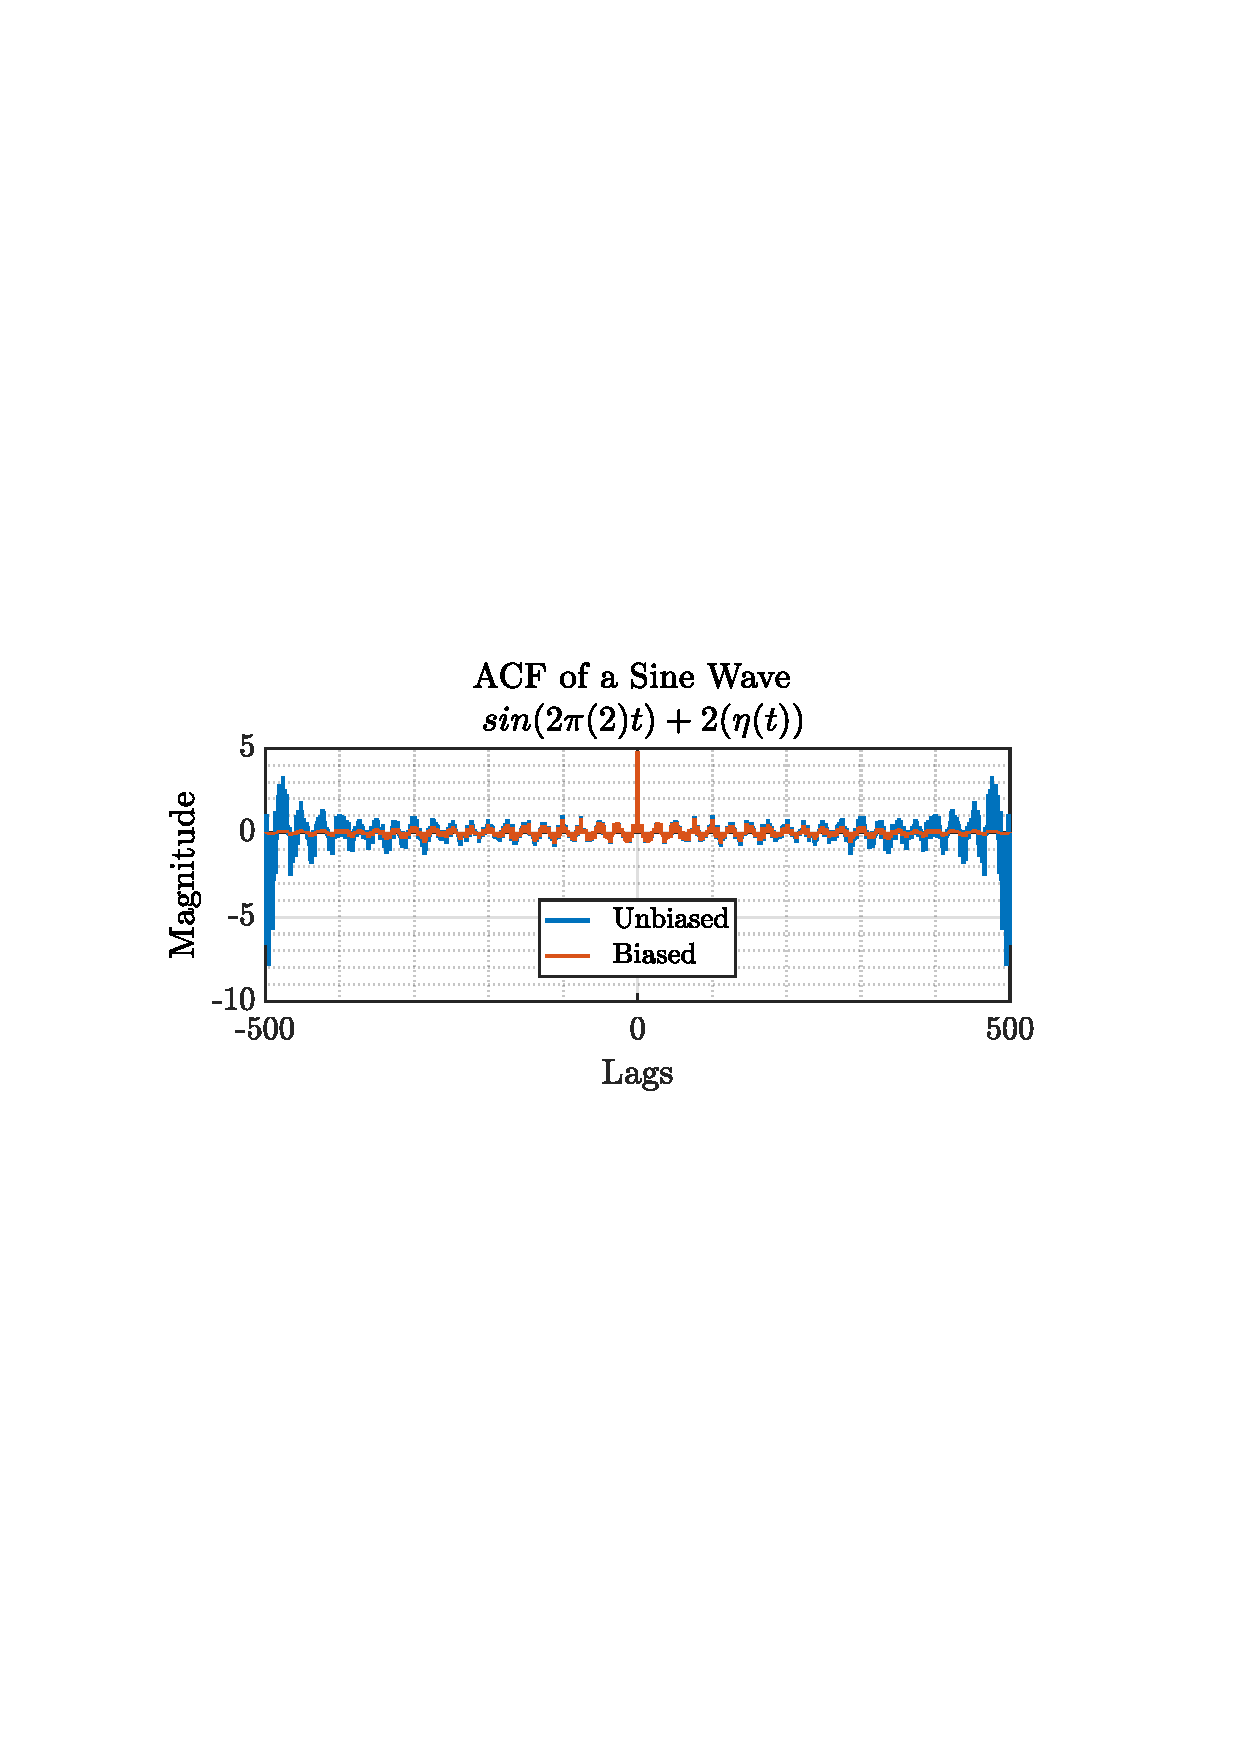
\includegraphics[trim={2.2cm 11.2cm 3.15cm  11.2cm}, clip, width=\textwidth]{../MATLAB/figures/q1_1b_fig01.pdf} 
		\captionsetup{justification=centering}
		\caption{An example of the Limiting Case of the Periodogram Definition}
		\label{fig: 1-1b}
	\end{figure}
	
	
	\subsection{Periodogram-based Methods Applied to Real–World Data} \label{sec: 1-2-PSD-real-world}
	\subsubsection{The SunSpot Dataset}
	Figure \ref{fig: 1-2a}. The mean's influence on data is the offset DC bias, captured in the $f=0$ component of the periodogram. Hence as we would expect, subtracting the \texttt{mean} reduces its magnitude in the periodogram. \texttt{detrend} removes linear trends, it seems in the case of this data set that most linear trends are captured at $f\lessapprox 0.02 rad/sample$. \\
	
	The natural logarithm was taken using: \texttt{log}. As the logarithm has a compression effect on magnitude we see that the magnitude of both raw and periodogram is greatly attenuated. We note that frequencies of interest and its harmonics appear as more distinct when compared to the rest of the periodogram.

	\begin{figure}[H]
		\centering
		\begin{subfigure}{0.49\textwidth}
			\centering
			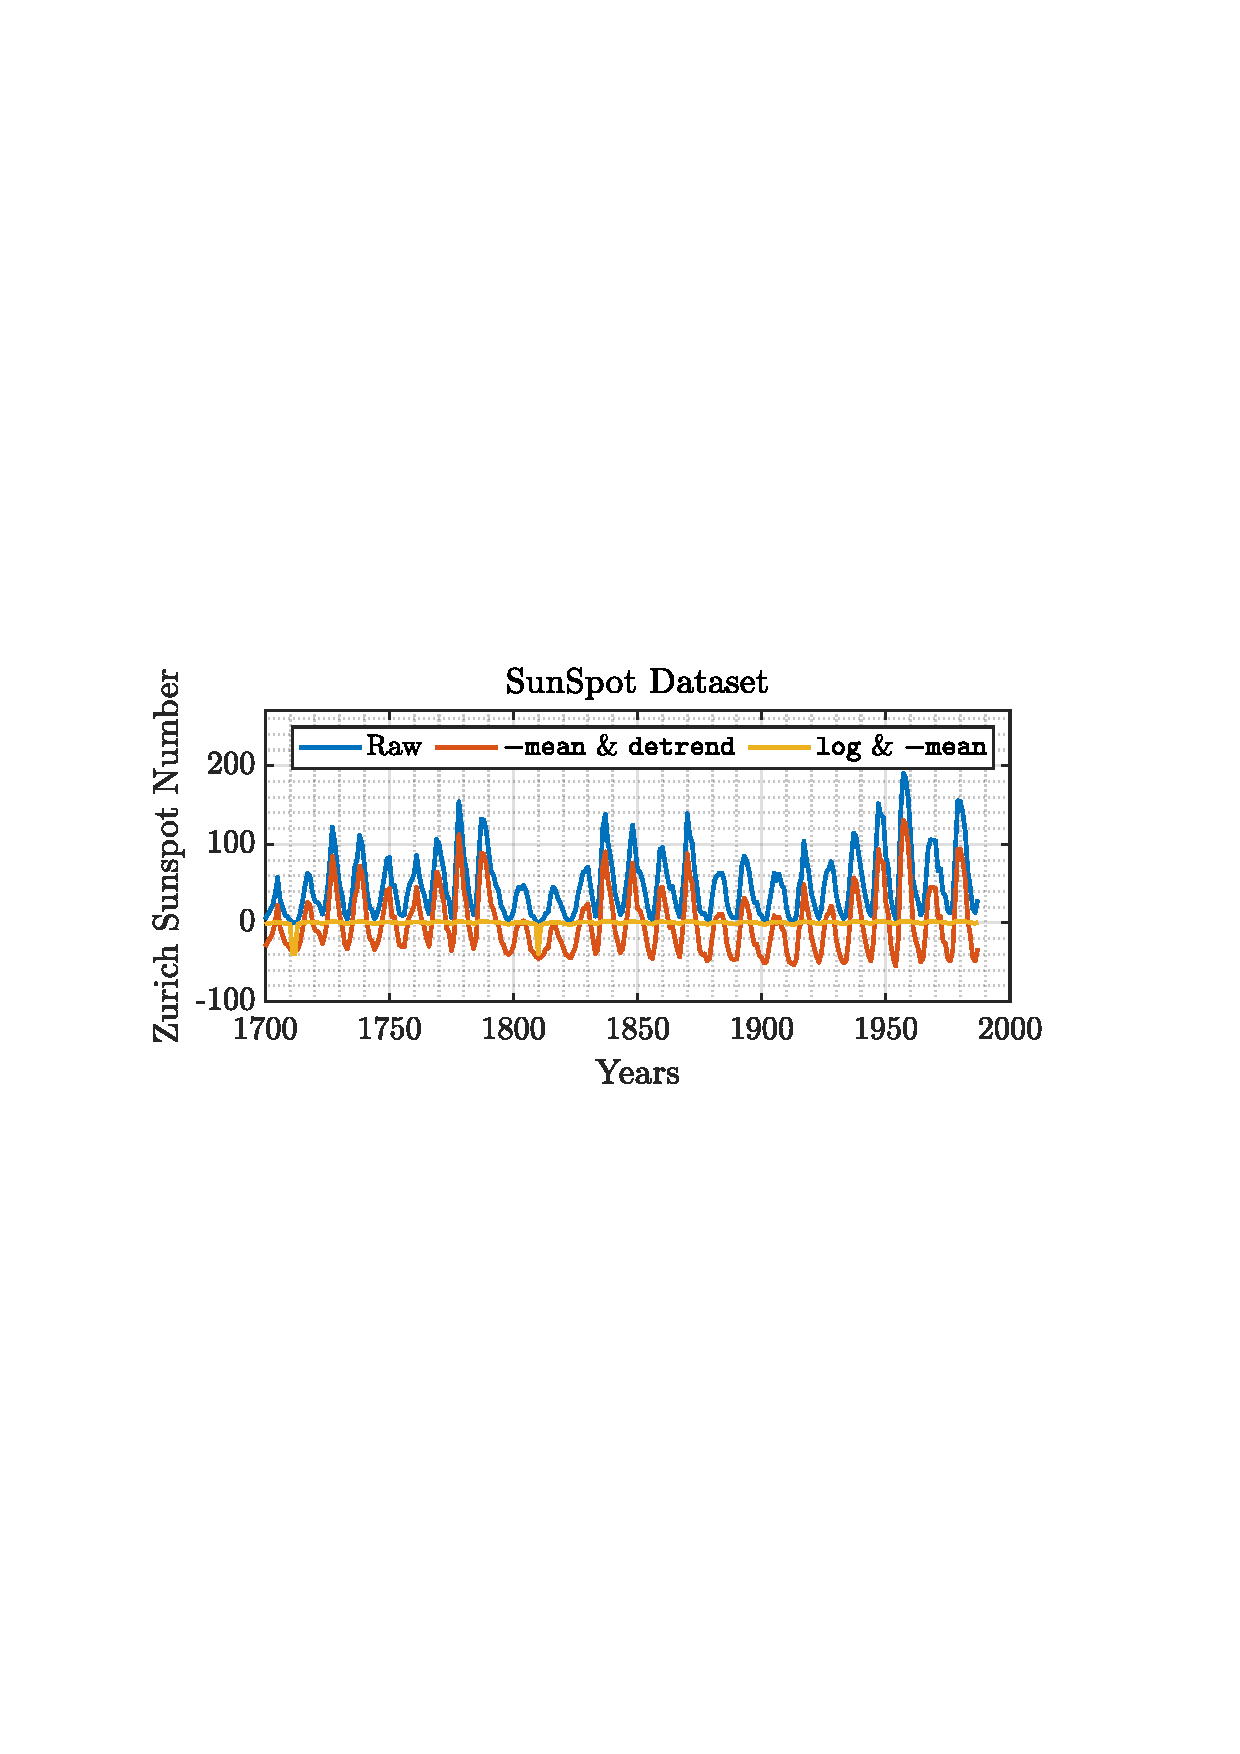
\includegraphics[trim={2.2cm 11.2cm 3.15cm  11.2cm}, clip, width=\textwidth]{../MATLAB/figures/q1_2a_fig01.pdf} 
			\captionsetup{justification=centering}
			\caption{Raw and its preprocessed datas}
		\end{subfigure}
%		~ % forces onto the same row
		\begin{subfigure}{0.49\textwidth}
			\centering
			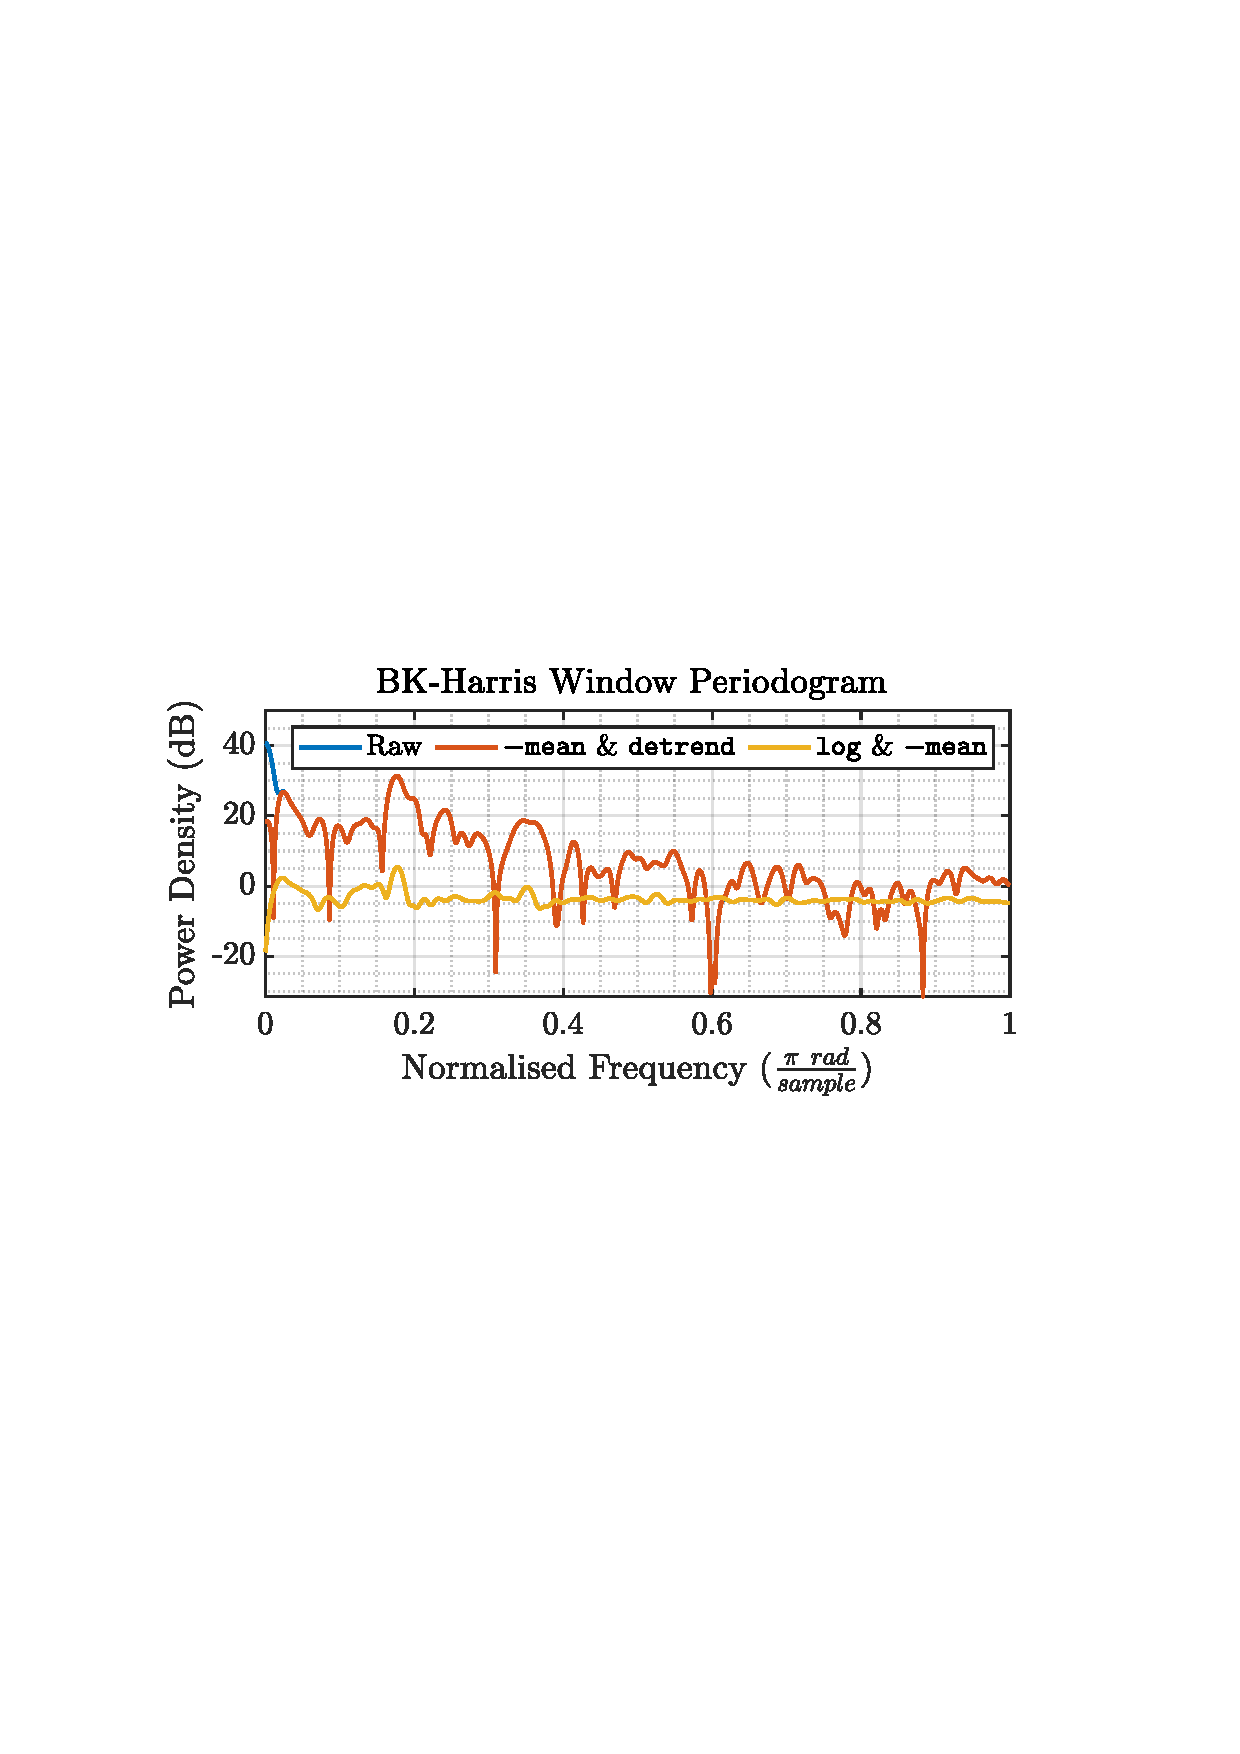
\includegraphics[trim={2.2cm 11.2cm 3.15cm  11.2cm}, clip, width=\textwidth]{../MATLAB/figures/q1_2a_fig02.pdf} 
			\captionsetup{justification=centering}
			\caption{Periodograms}
		\end{subfigure}
		\captionsetup{justification=centering}
		\caption{}
		\label{fig: 1-2a}
	\end{figure}
%	\begin{figure}[H]
%		\centering
%		%\begin{subfigure}[t]{0.4\textwidth}
%		%	\centering
%		%\hspace*{-2.1cm}
%		% 				trim={<left> <lower> <right> <upper>}
%		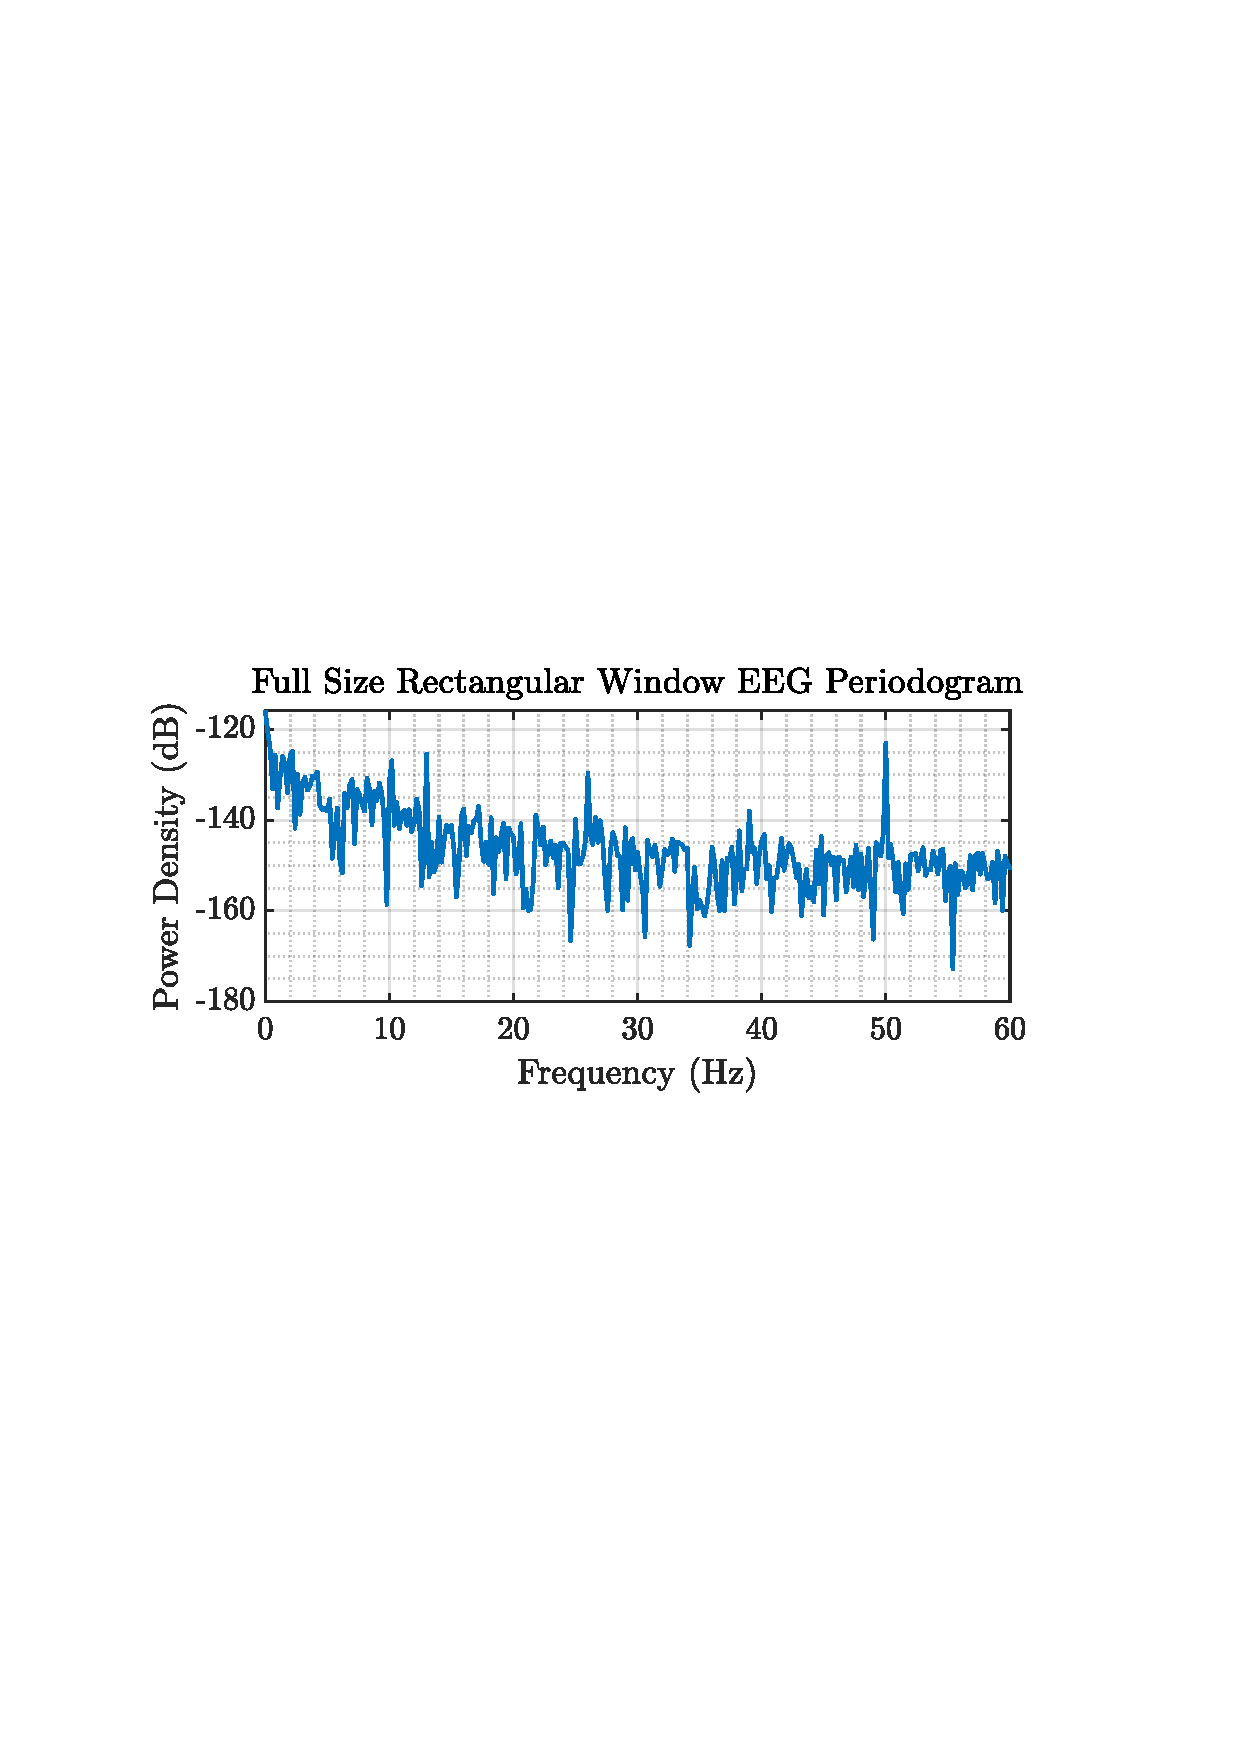
\includegraphics[trim={2.2cm 11.2cm 3.15cm  11.2cm}, clip, width=9cm]{../MATLAB/figures/q1_2b_fig01.pdf} 
%		%	\captionsetup{justification=centering}
%		%	\caption{Vertical gel electrophoresis setup} 
%		%	\label{fig: verticalGel}
%		%\end{subfigure}
%		%\hfill
%		\captionsetup{justification=centering}
%		\caption{Science being done here}
%	\end{figure}


	\subsubsection{The EEG Dataset}
	
	\begin{figure}[H]
		\centering
		\begin{subfigure}{0.49\textwidth}
			\centering
			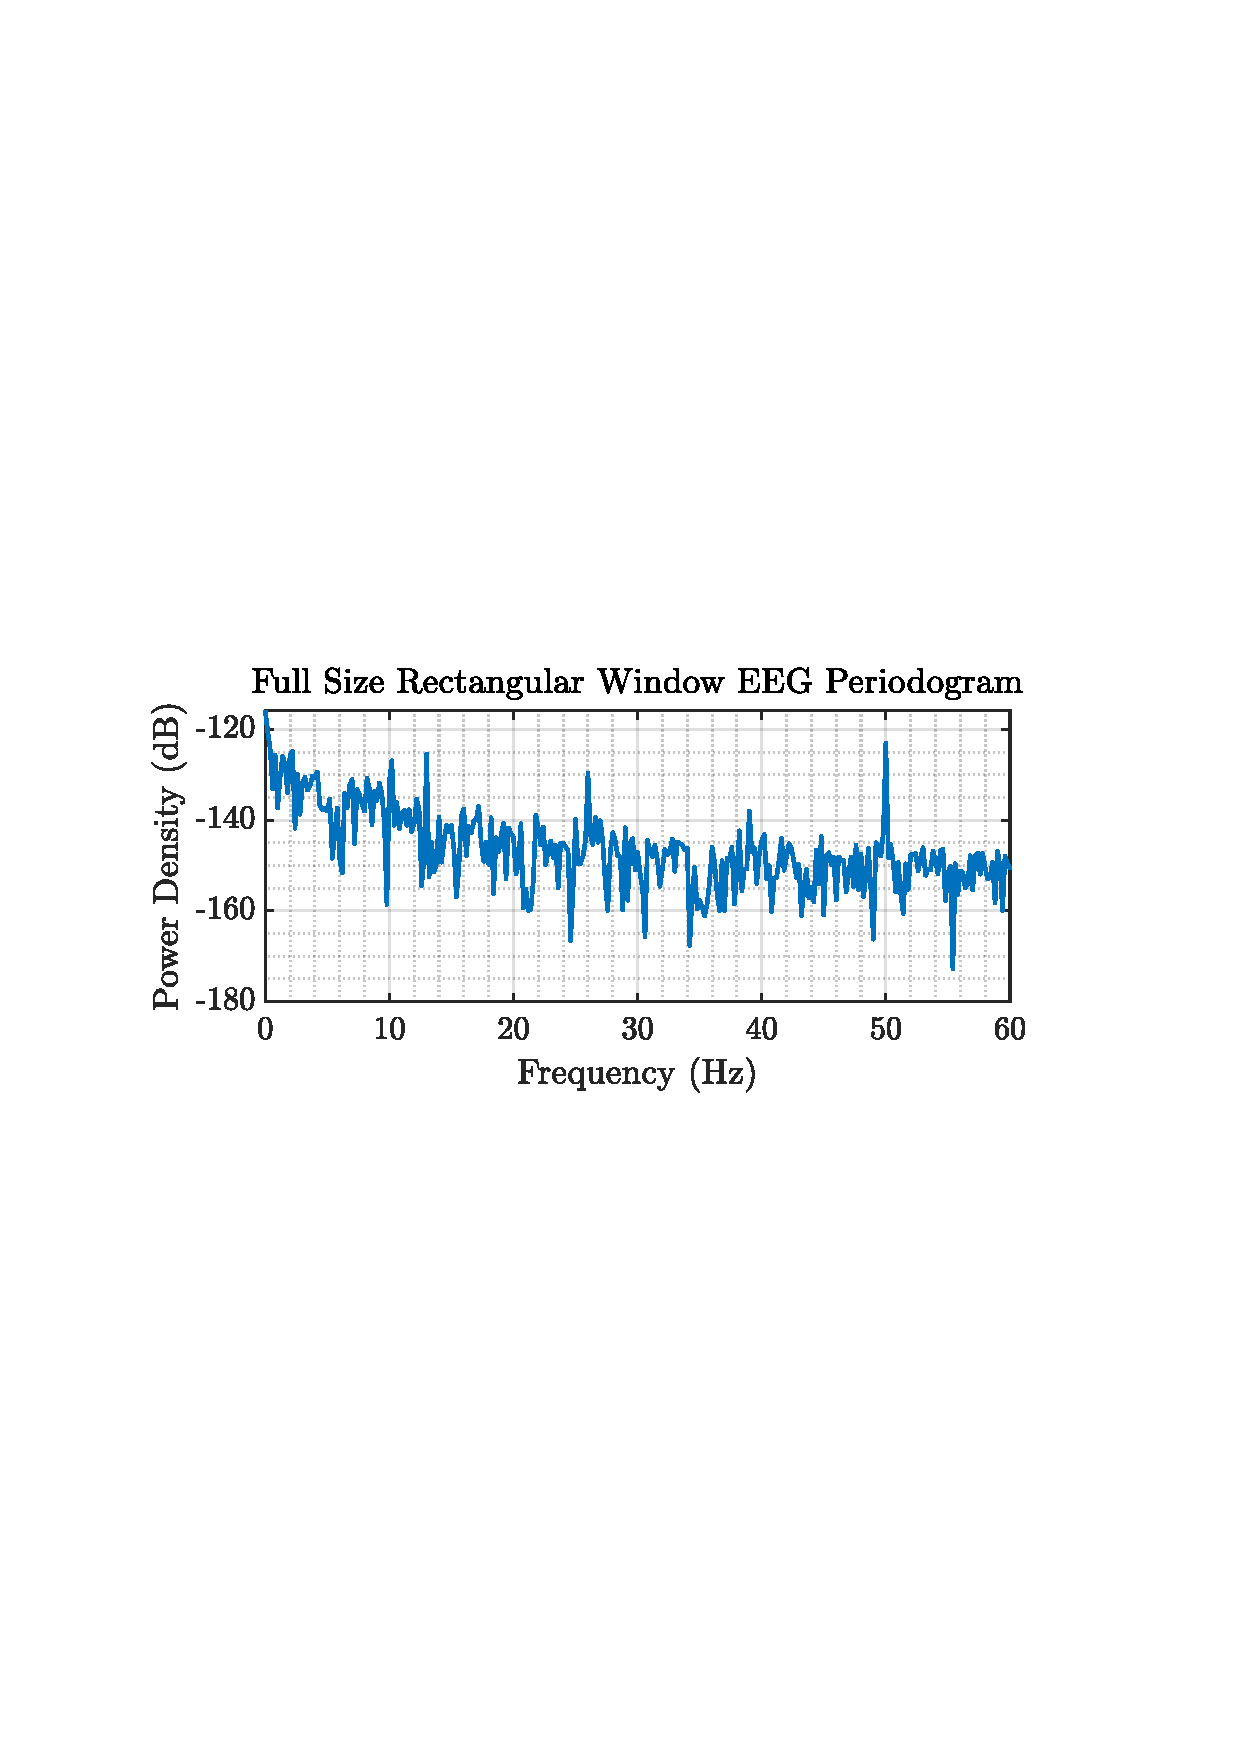
\includegraphics[trim={2.2cm 11.2cm 3.15cm  11.2cm}, clip, width=\textwidth]{../MATLAB/figures/q1_2b_fig01.pdf} 
			\captionsetup{justification=centering}
			\caption{Standard Periodogram}
		\end{subfigure}
		%		~ % forces onto the same row
		\begin{subfigure}{0.49\textwidth}
			\centering
			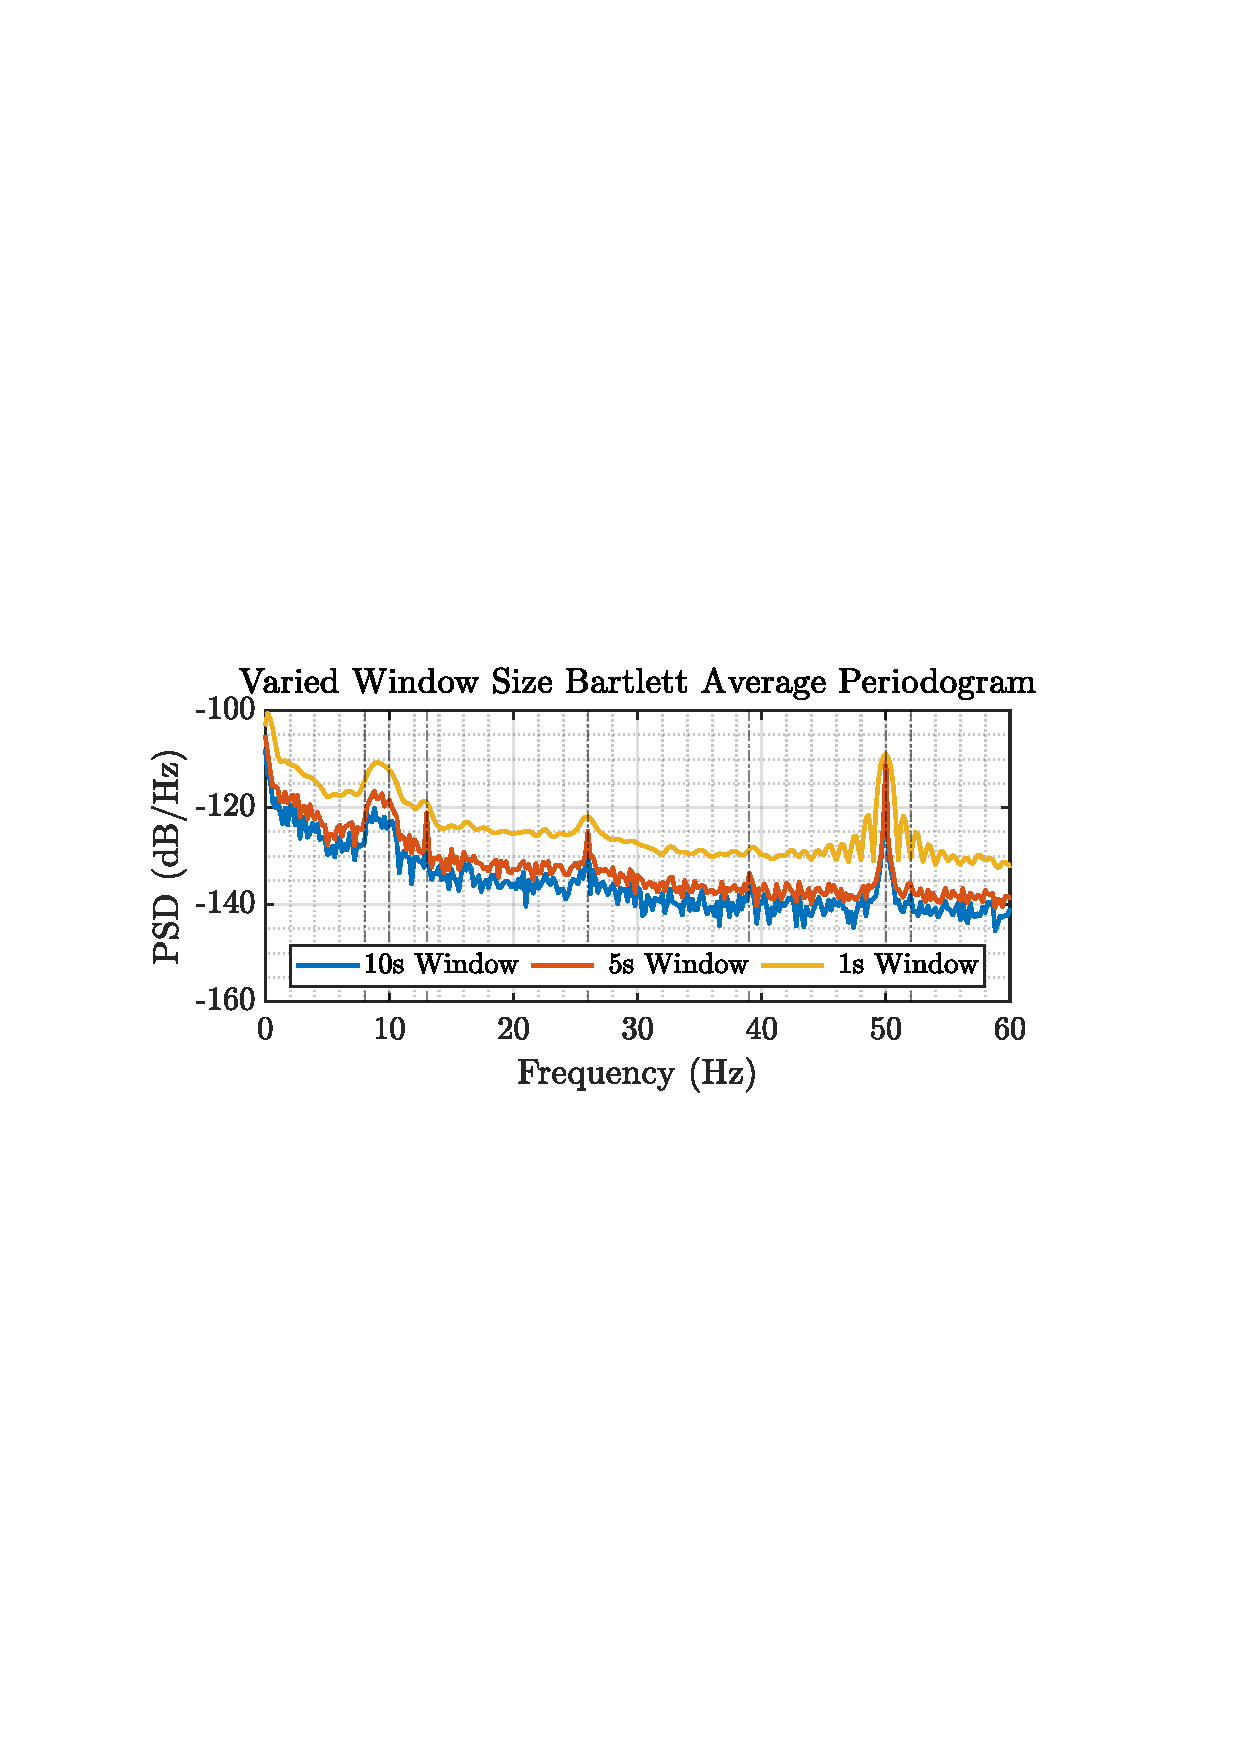
\includegraphics[trim={2.2cm 11.2cm 3.15cm  11.2cm}, clip, width=\textwidth]{../MATLAB/figures/q1_2b_fig02.pdf} 
			\captionsetup{justification=centering}
			\caption{Bartlett Average Periodograms}
		\end{subfigure}
		\captionsetup{justification=centering}
		\caption{}
		\label{fig: 1-2b}
	\end{figure}

	\begin{table}[H]
		\centering
		\begin{tabular}{|c|c||c|}
			\hline
			\textbf{Response} & \textbf{Expected Range} (Hz) & \textbf{Observed Range} (Hz) \\
			\hline
			\hline
			{Alpha Rhythm} & $8 - 10$ & $8-10$ \\
			\hline
			{SSVEP} & \texttt{range}[$11-20$] & $13n$ \\
			\hline
			{Power-Line} & $50$ & $50$ \\
			\hline
		\end{tabular}
		\captionsetup{justification=centering}
		\caption{EEG Frequency Peaks of the Periodogram. $n$ refers to harmonics}
		\label{tab: 1-2b}
	\end{table}
	
	The standard periodogram has identifiable peaks, showing in Figure \ref{fig: 1-2b}, quantified in Table \ref{tab: 1-2b}. We are unable to identify the 3rd harmonic of the SSVEP, at 52Hzs it is too close to the power-line interference at 50Hz. The main difference in the 10s window averaged periodogram is clearer peak isolation compared to the surrounding periodogram and emphasis on the range of frequencies of the alpha-rhythm, rather than a single discrete peak.

	\subsection{Correlation Estimation} \label{sec: 1-3-correlation-est}
	
	\subsubsection{Unbiased and Biased ACF Estimates}
	
	\begin{figure}[H]
		\centering
		\begin{subfigure}{0.49\textwidth}
			\centering
			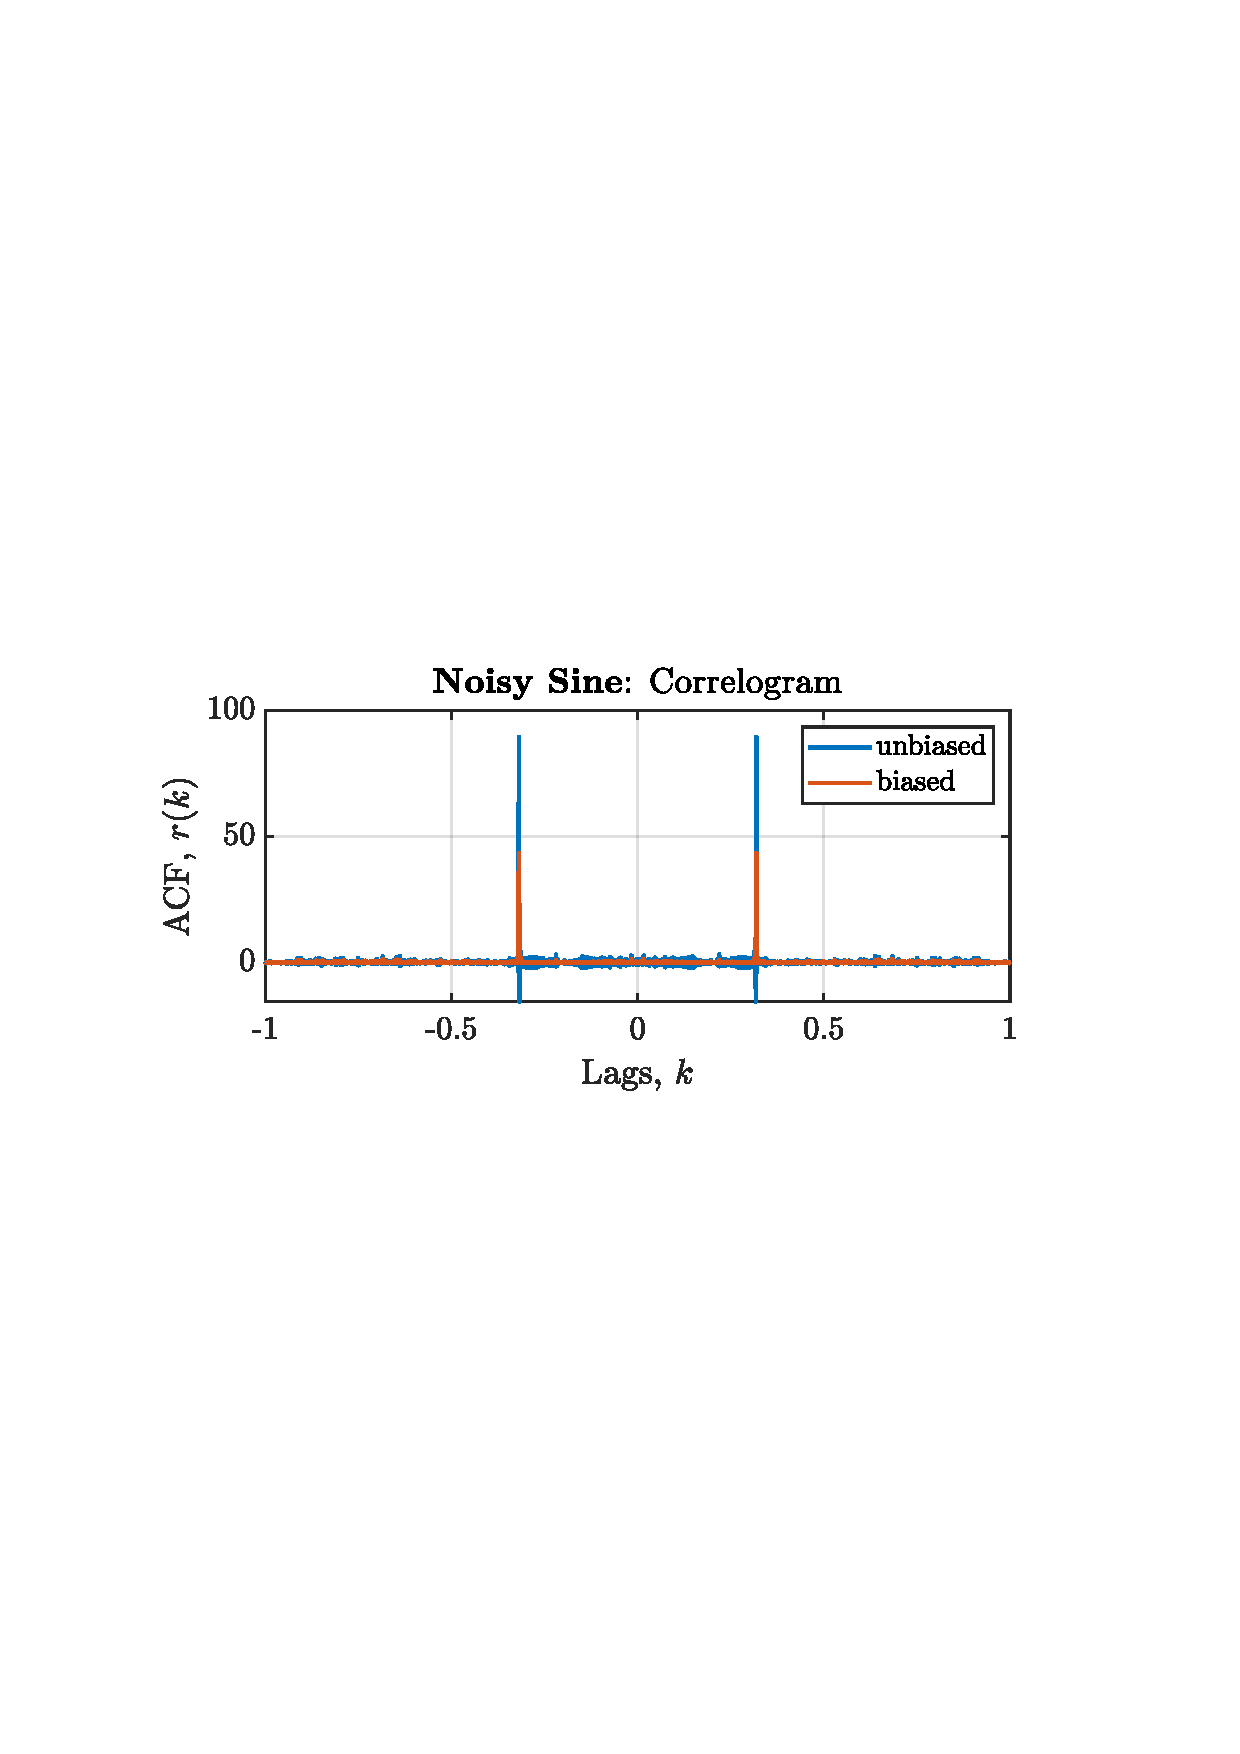
\includegraphics[trim={2.2cm 11cm 3.15cm  11.2cm}, clip, width=\textwidth]{../MATLAB/figures/q1_3a_fig04.pdf} 
		\end{subfigure}
		%		~ % forces onto the same row
		\begin{subfigure}{0.49\textwidth}
			\centering
			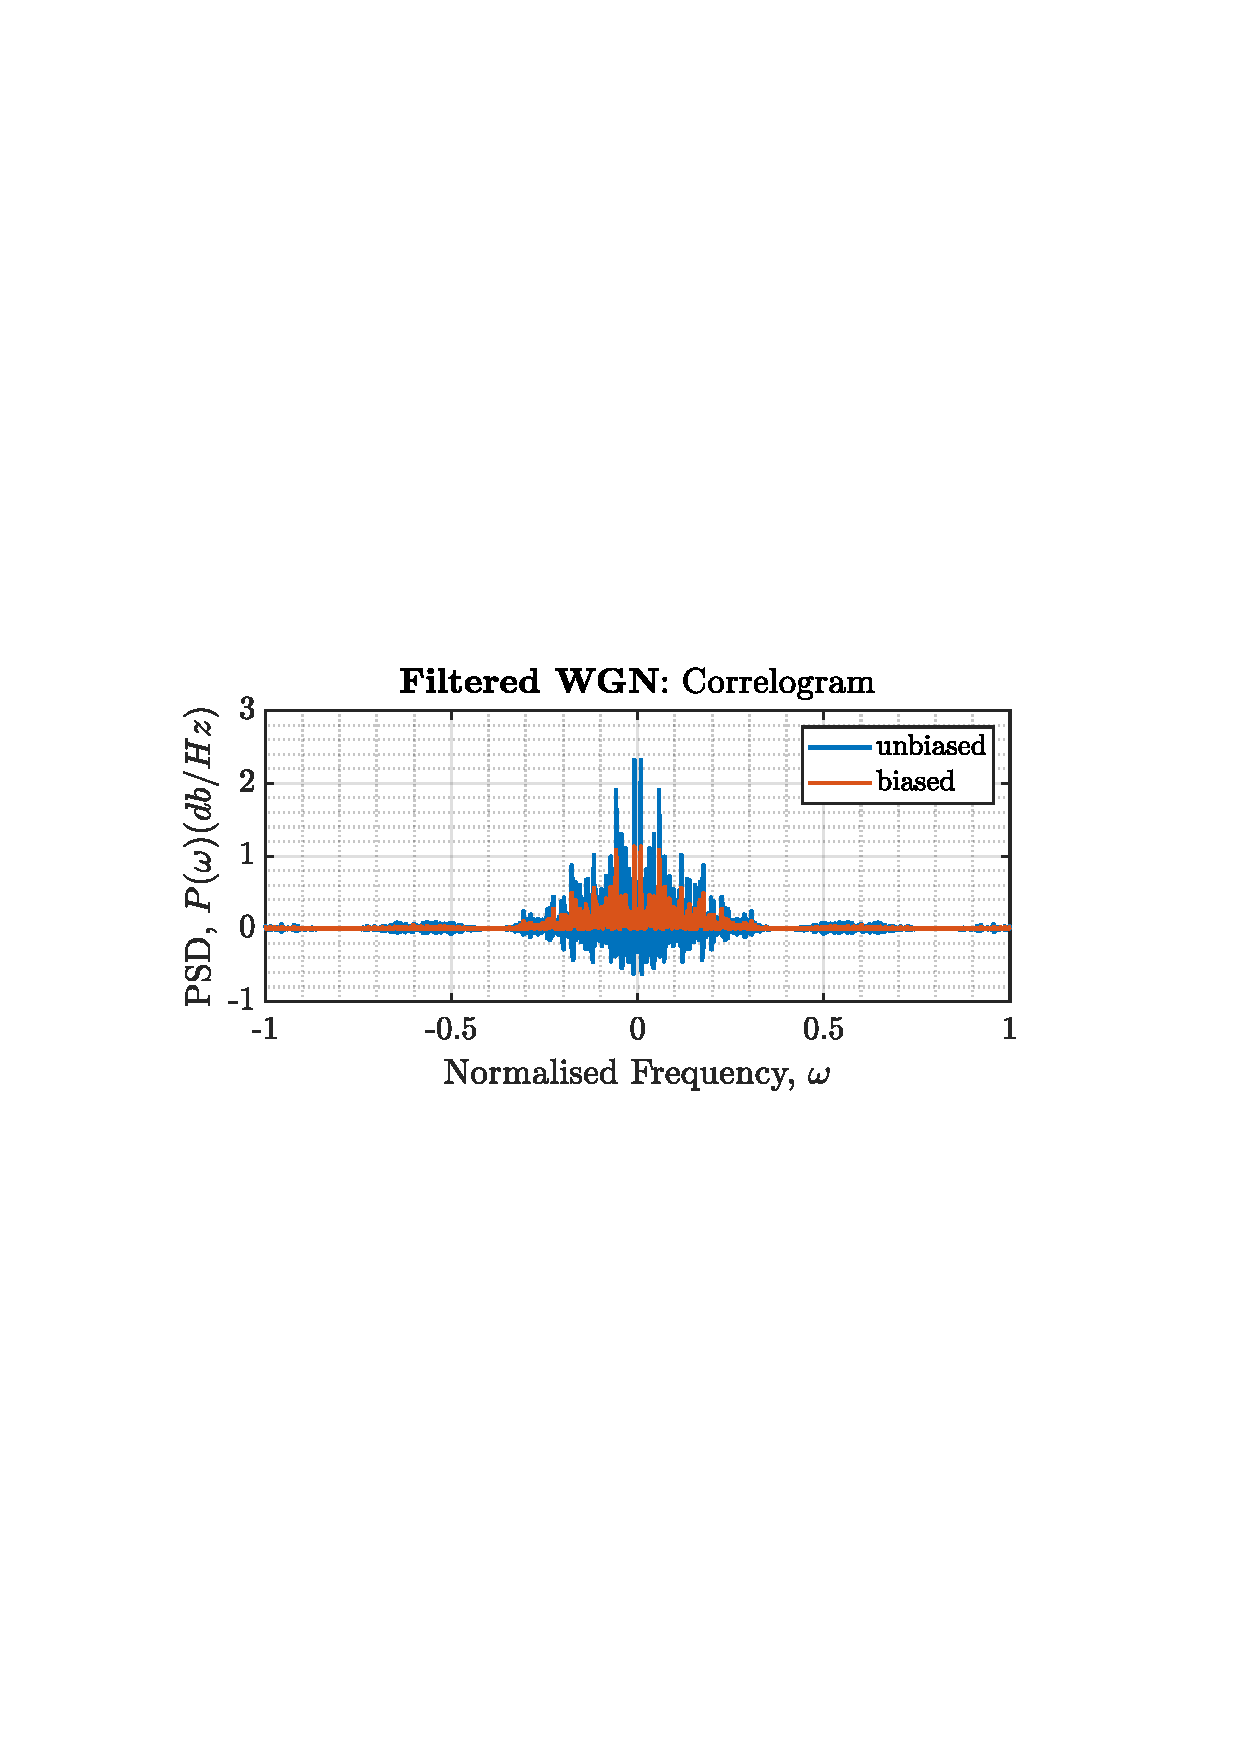
\includegraphics[trim={2.2cm 11cm 3.15cm  11.2cm}, clip, width=\textwidth]{../MATLAB/figures/q1_3a_fig05.pdf} 
		\end{subfigure}
				\begin{subfigure}{0.49\textwidth}
			\centering
			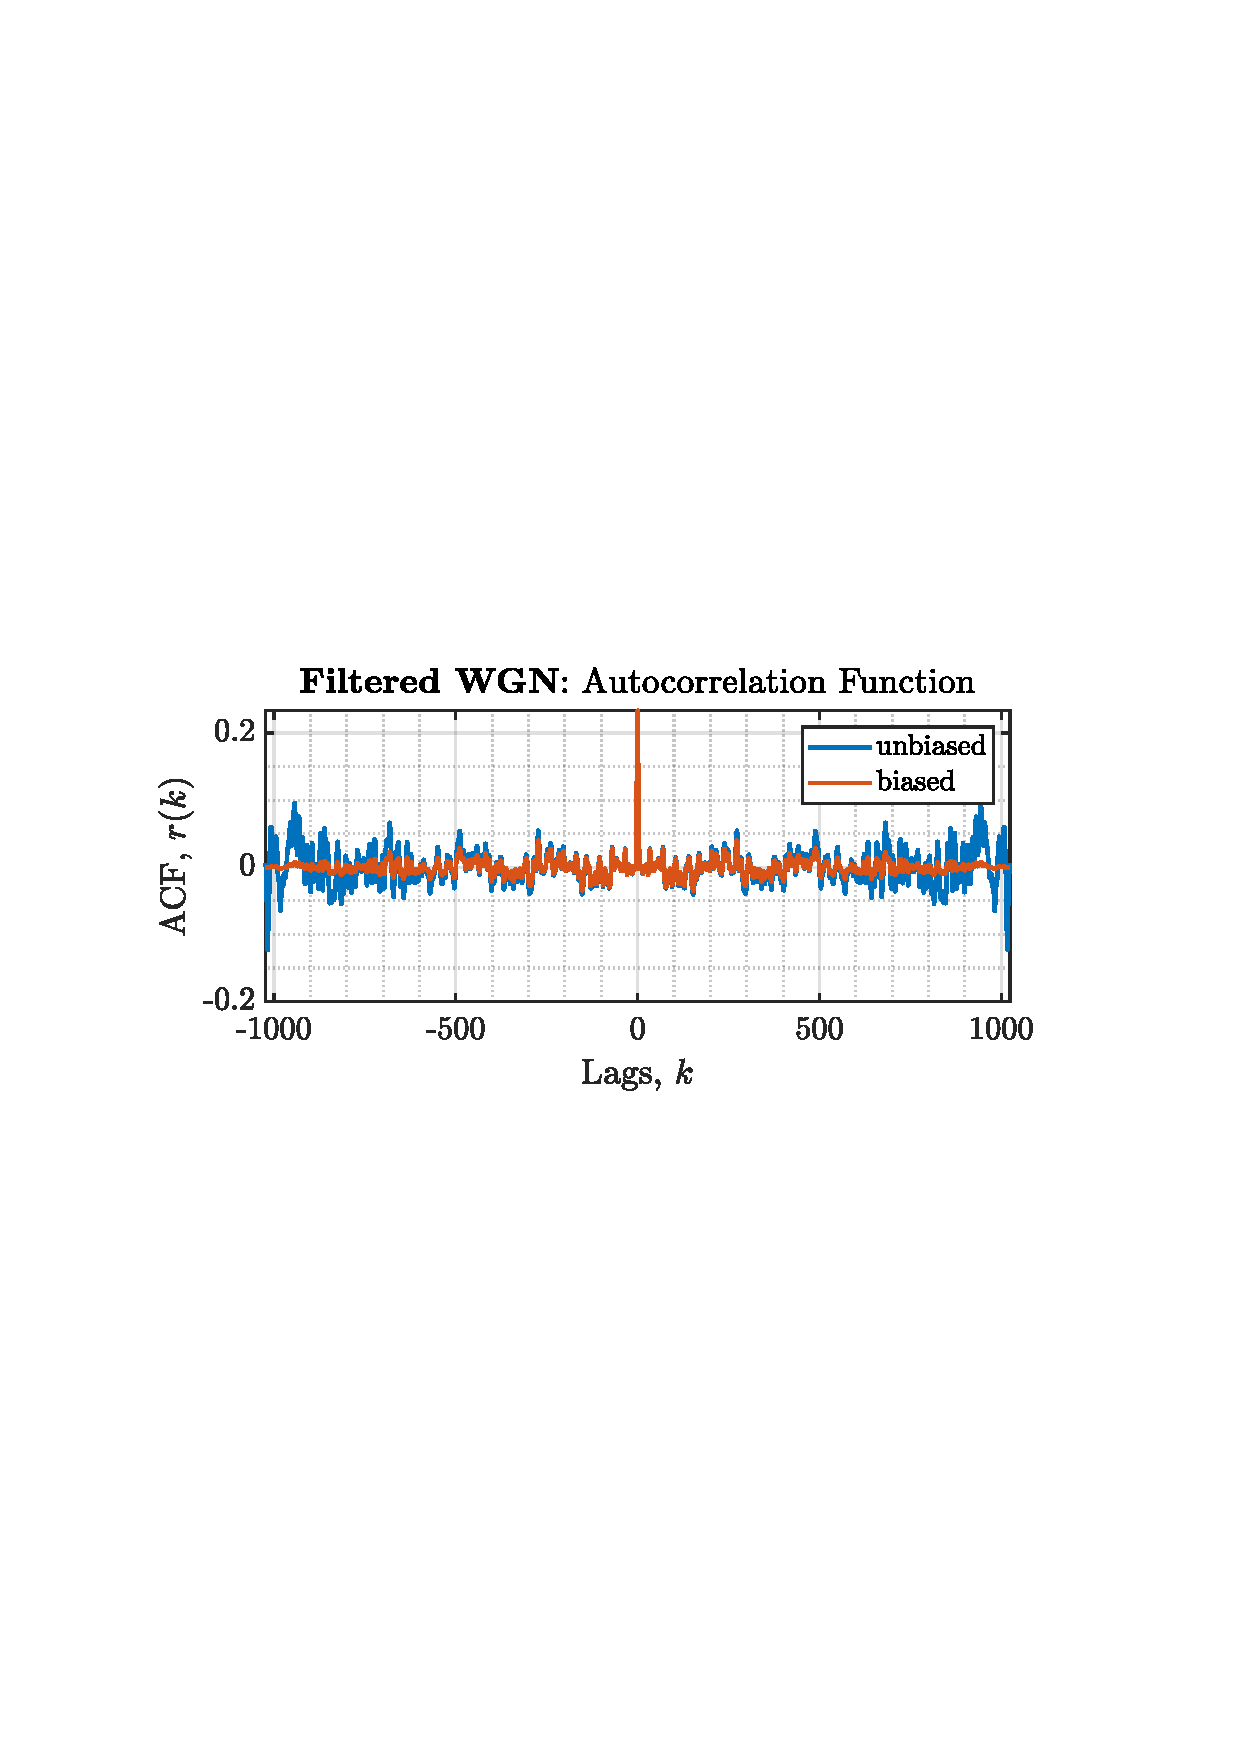
\includegraphics[trim={2.2cm 11cm 3.15cm  11.2cm}, clip, width=\textwidth]{../MATLAB/figures/q1_3a_fig06.pdf} 
		\end{subfigure}
		%		~ % forces onto the same row
		\begin{subfigure}{0.49\textwidth}
			\centering
			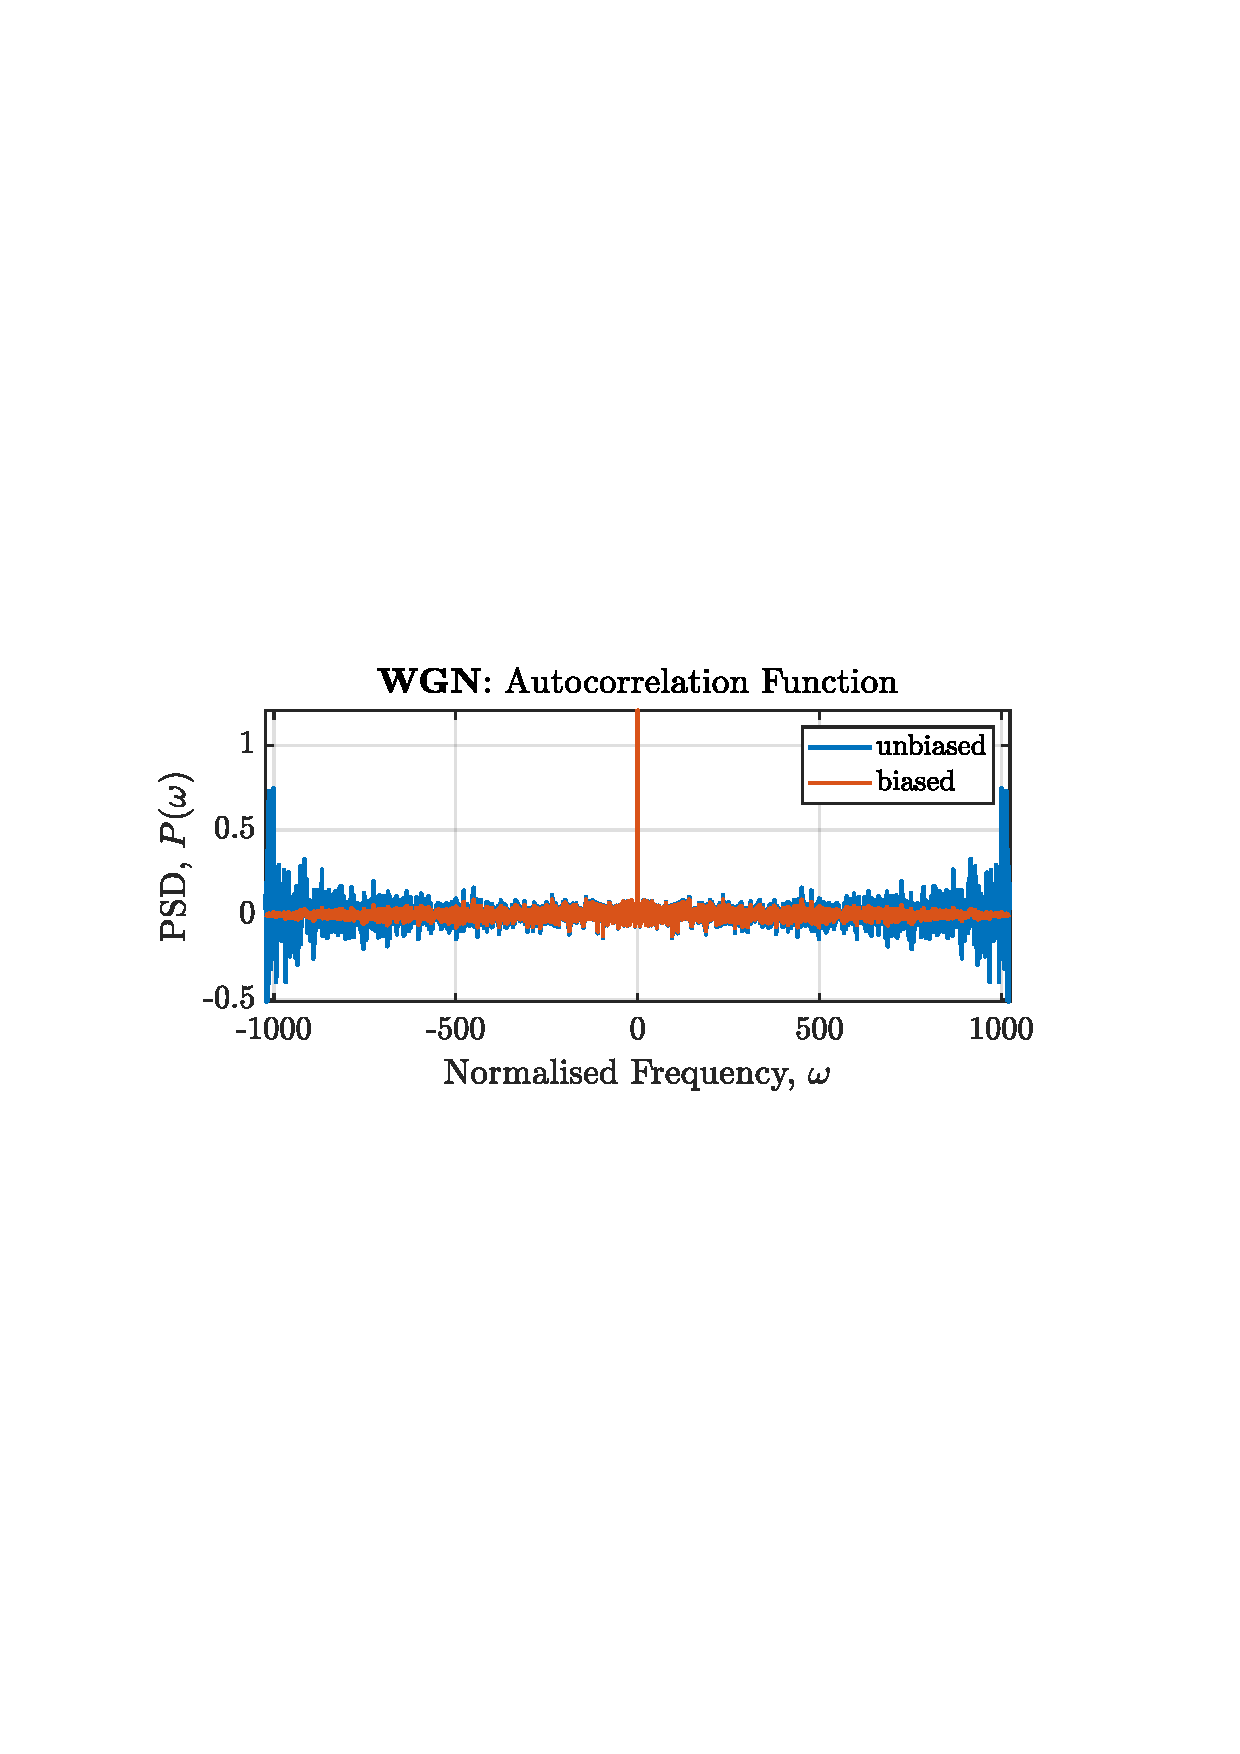
\includegraphics[trim={2.2cm 11cm 3.15cm  11.2cm}, clip, width=\textwidth]{../MATLAB/figures/q1_3a_fig01.pdf} 
		\end{subfigure}
		\begin{subfigure}{0.49\textwidth}
			\centering
			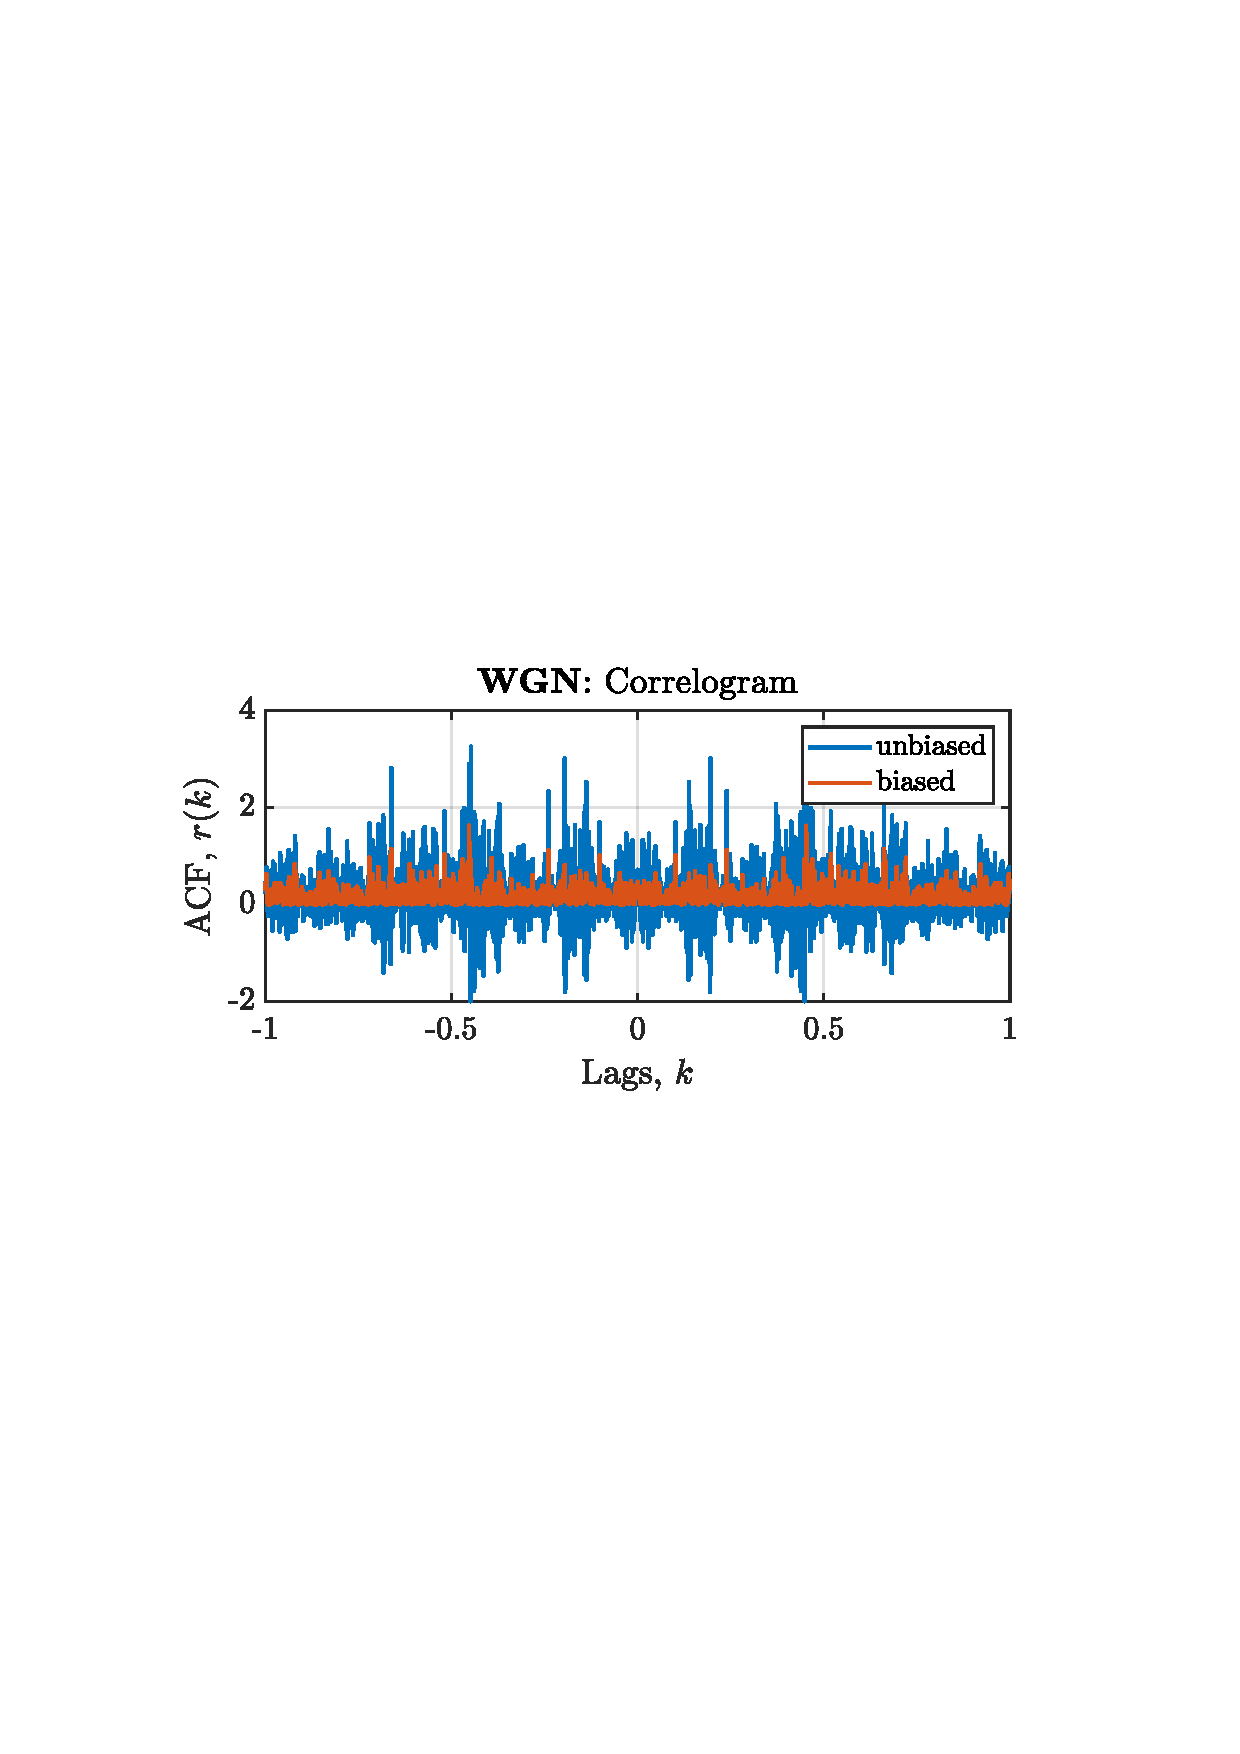
\includegraphics[trim={2.2cm 11.2cm 3.15cm  11.2cm}, clip, width=\textwidth]{../MATLAB/figures/q1_3a_fig02.pdf} 
		\end{subfigure}
		%		~ % forces onto the same row
		\begin{subfigure}{0.49\textwidth}
			\centering
			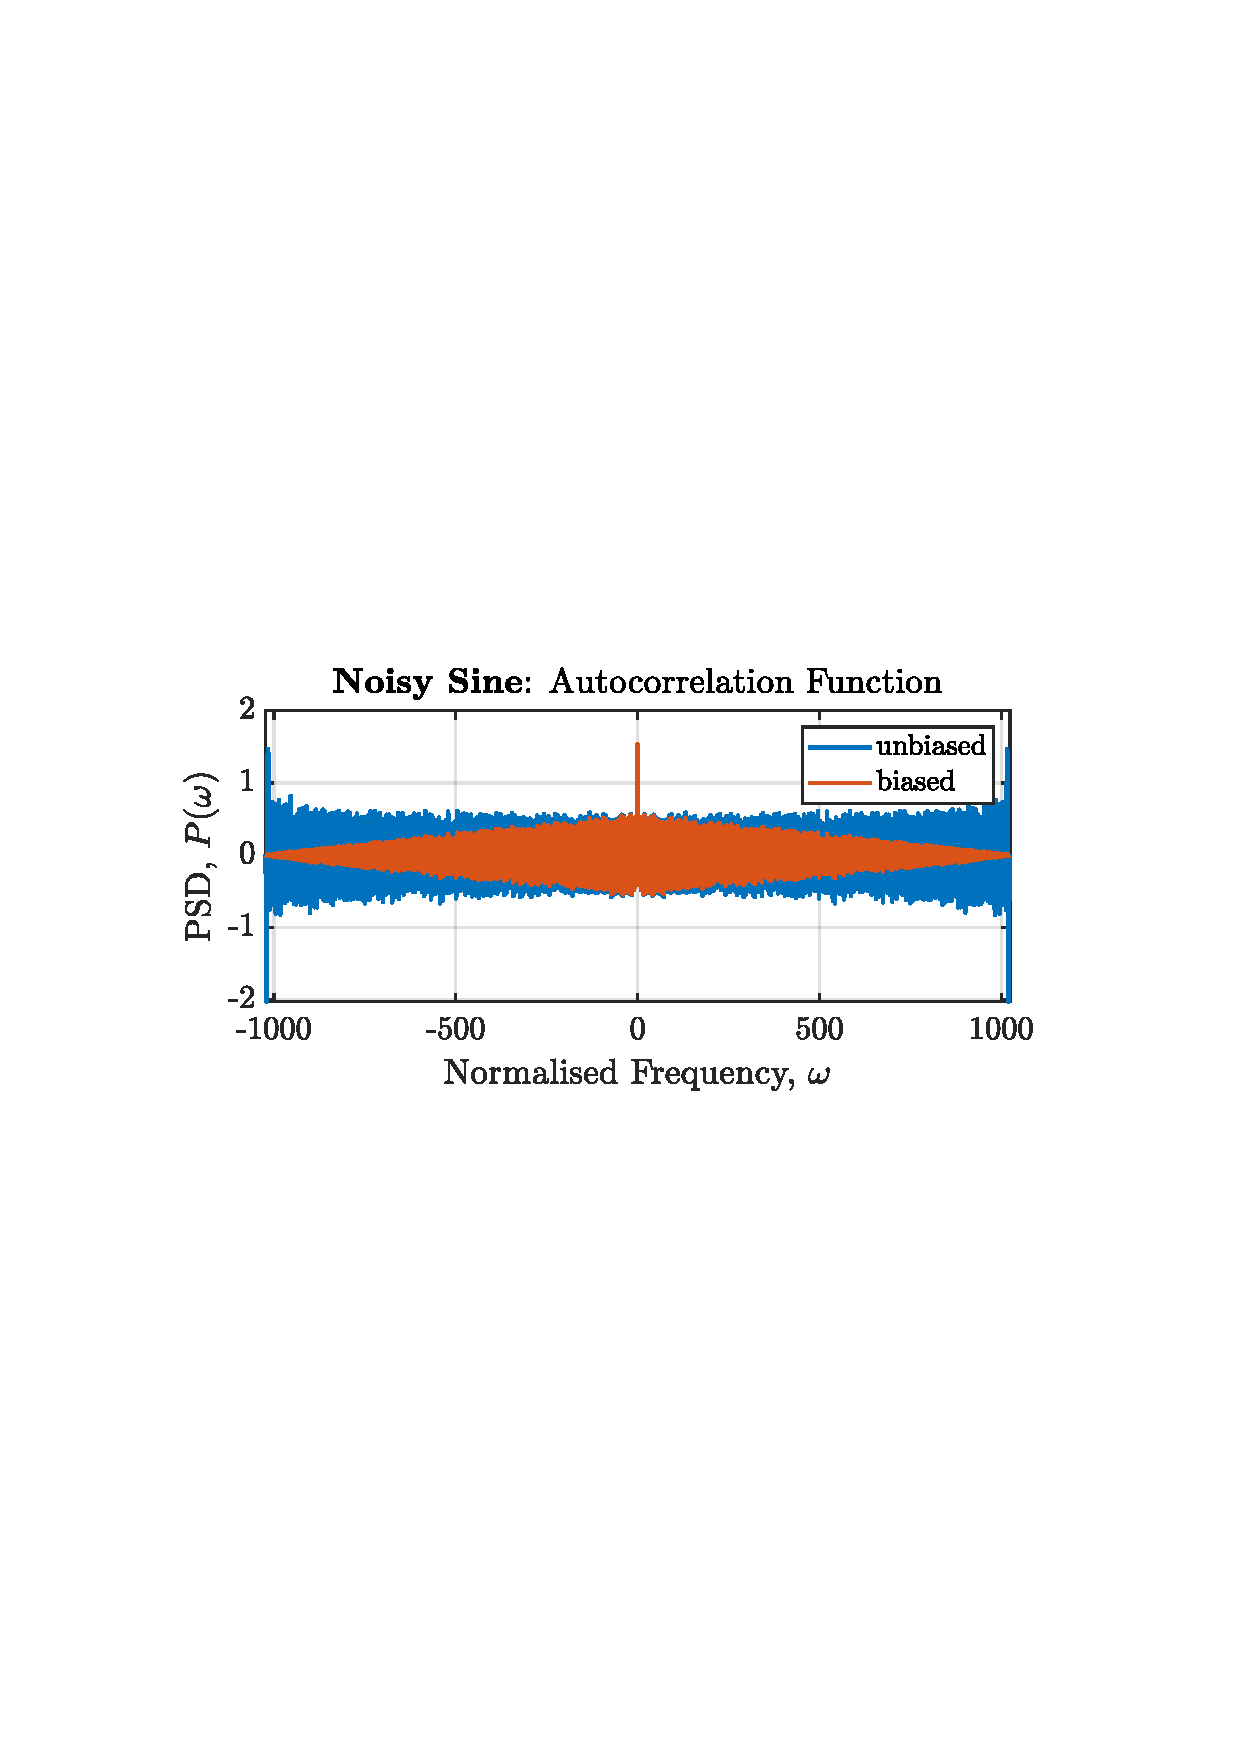
\includegraphics[trim={2.2cm 11.2cm 3.15cm  11.2cm}, clip, width=\textwidth]{../MATLAB/figures/q1_3a_fig03.pdf} 
		\end{subfigure}
		\captionsetup{justification=centering}
		\caption{Set of Auto-Correlation Functions (ACFs) and their Correlograms}
		\label{fig: 1-3a}
	\end{figure}
	
	Figure \ref{fig: 1-3a}. For the autocorrelation functions: we can see that the biased estimator tends to 0 for increasing lag magnitude, whereas the unbiased estimator remains somewhat constant, although at the extremes it begins to increase to approximately double the constant value.\\
	For the correlograms: we observe that the biased estimator does not contain negative values.
	
	\subsubsection{Biased ACF Estimator PSDs}

	The process simulated was the following:
	
	\begin{equation}
		\begin{aligned}
		x(n) = & 2 sin(2 \pi 0.4 n) + 1.75 sin(2 \pi 0.6 n) \\
		&  + 0.85 sin(2 \pi 0.85 n) + 1.2 sin(2 \pi 0.95 n) + \eta(n) \quad \eta \sim \mathcal{N}(0, 1)
		\end{aligned}
	\end{equation}
	
	

	\begin{figure}[H]
		\centering
		\begin{subfigure}{0.49\textwidth}
			\centering
			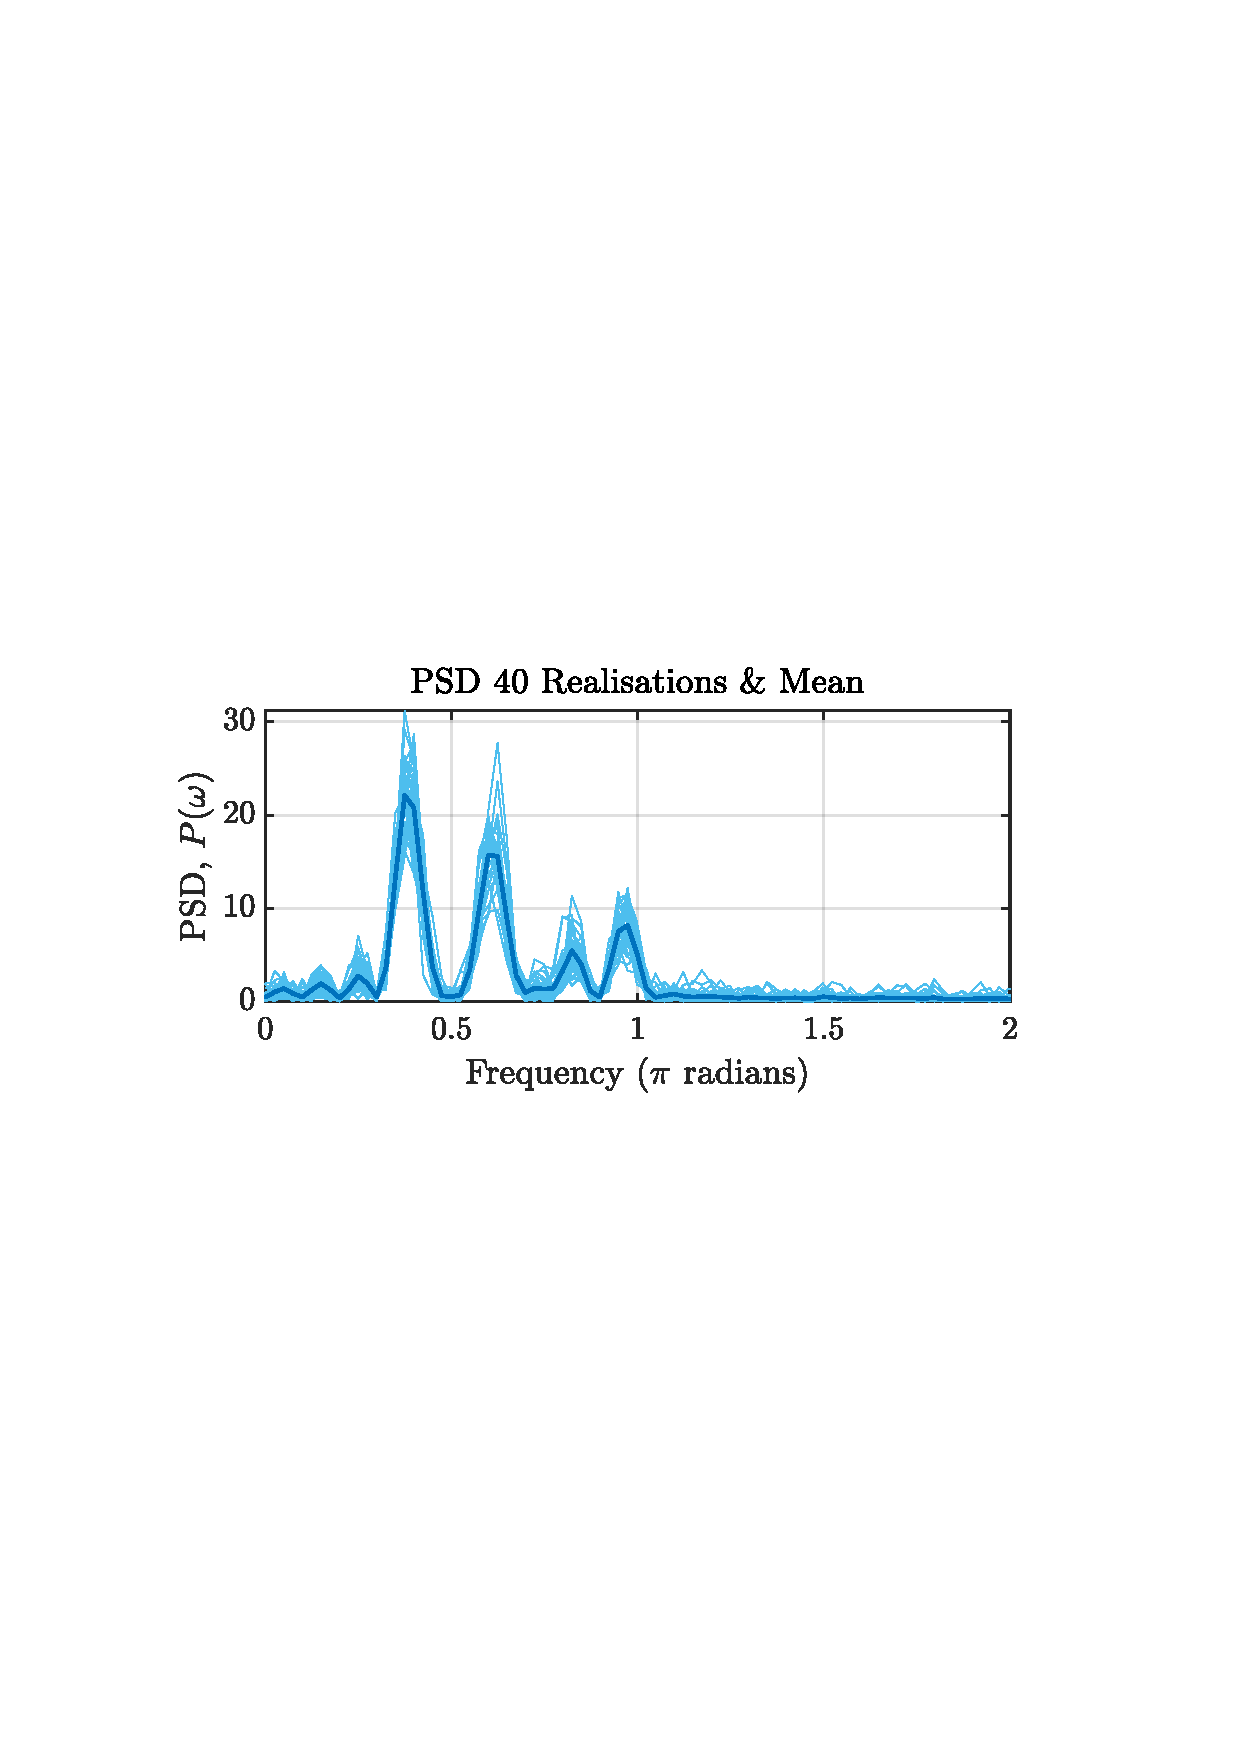
\includegraphics[trim={2.2cm 11.2cm 3.15cm  11.2cm}, clip, width=\textwidth]{../MATLAB/figures/q1_3b_fig01.pdf} 
			\captionsetup{justification=centering}
			\caption{Periodogram}
		\end{subfigure}
		%		~ % forces onto the same row
		\begin{subfigure}{0.49\textwidth}
			\centering
			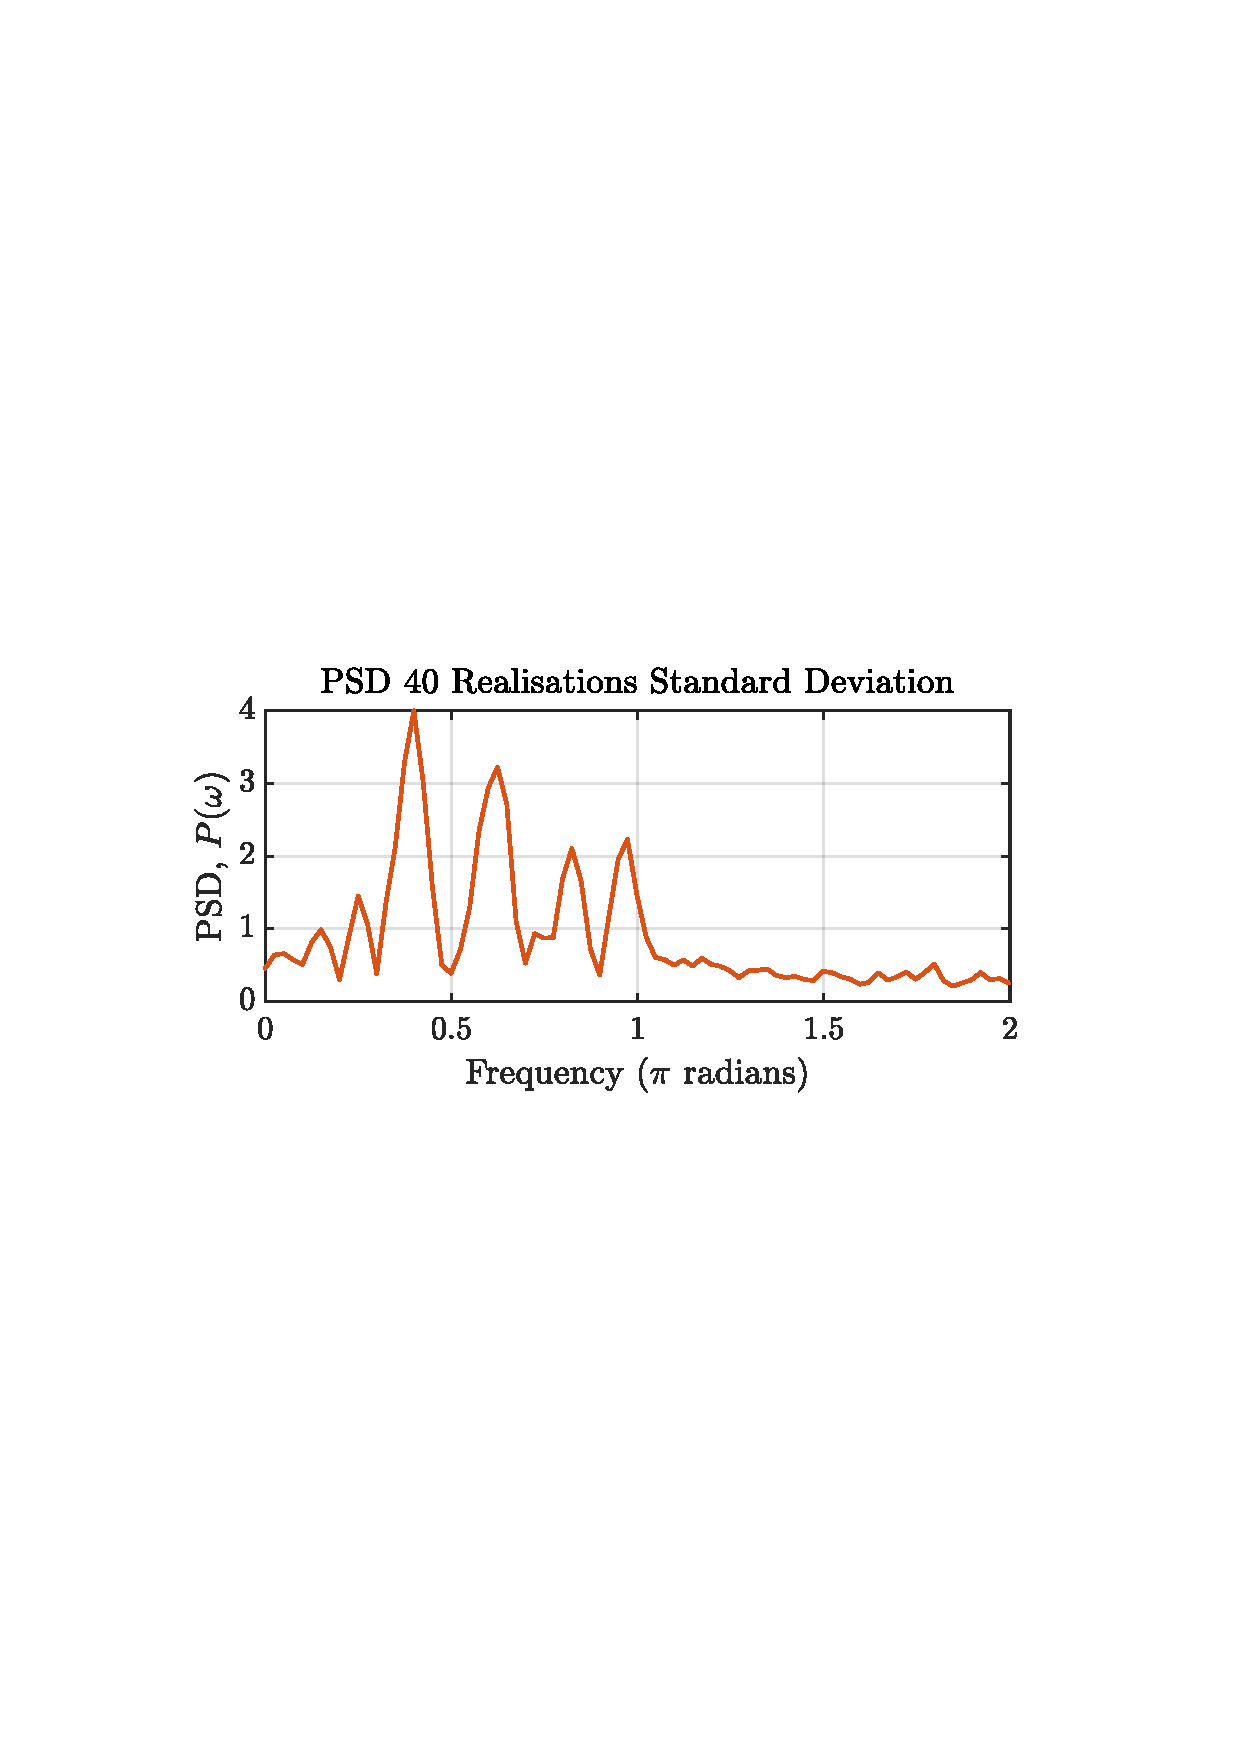
\includegraphics[trim={2.2cm 11.2cm 3.15cm  11.2cm}, clip, width=\textwidth]{../MATLAB/figures/q1_3b_fig02.pdf} 
			\captionsetup{justification=centering}
			\caption{Standard Deviation}
		\end{subfigure}
		\captionsetup{justification=centering}
		\caption{The total number of data points used was 512, black vertical lines indicate the model defined frequencies}
		\label{fig: 1-3b}
	\end{figure}

	It is interesting to see the low frequency resolution influences the accuracy of the peak with respect to the actual frequencies used, Figure \ref{fig: 1-3b}.

	\subsubsection{Biased ACF Estimator PSDs on the dB Scale}

	\begin{figure}[H]
		\centering
		\begin{subfigure}{0.49\textwidth}
			\centering
			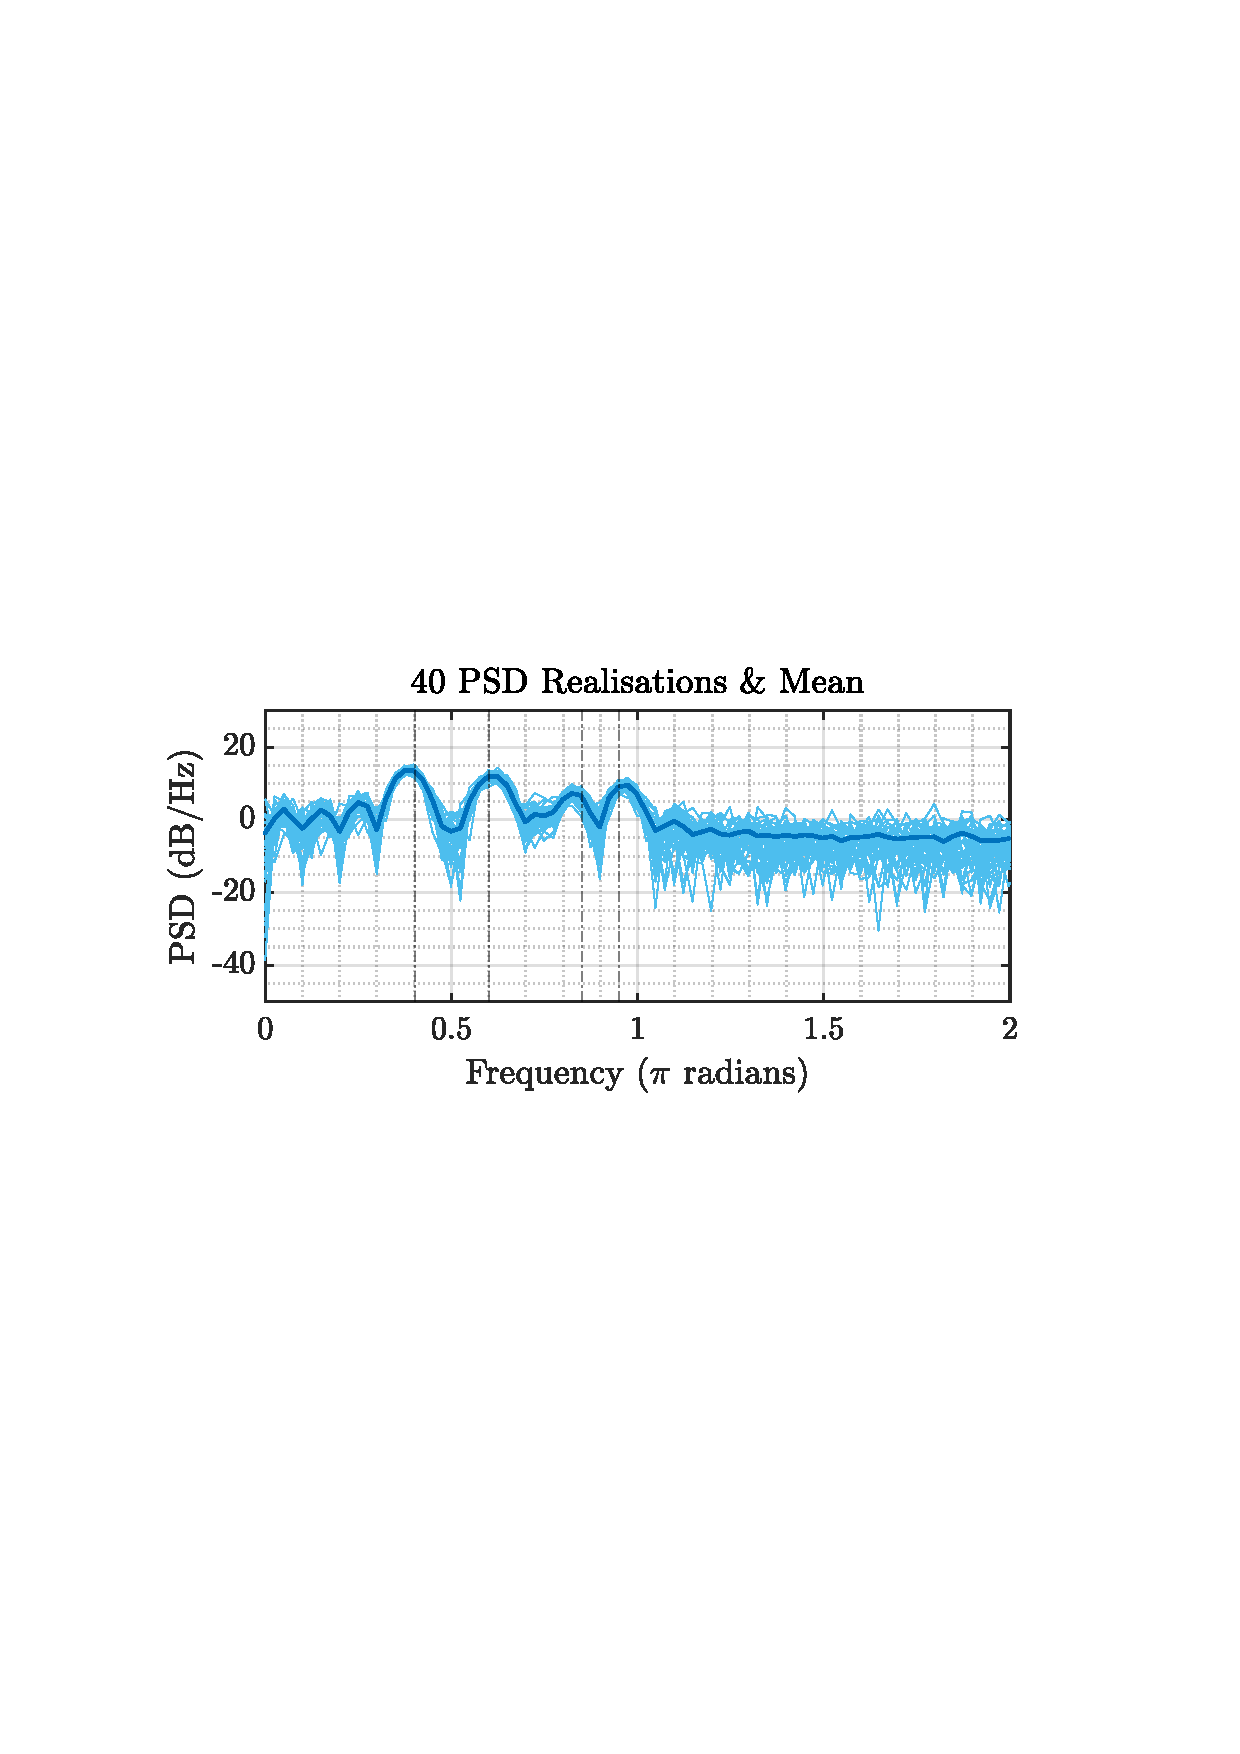
\includegraphics[trim={2.2cm 11.2cm 3.15cm  11.2cm}, clip, width=\textwidth]{../MATLAB/figures/q1_3c_fig01.pdf} 
			\captionsetup{justification=centering}
			\caption{Periodogram}
		\end{subfigure}
		%		~ % forces onto the same row
		\begin{subfigure}{0.49\textwidth}
			\centering
			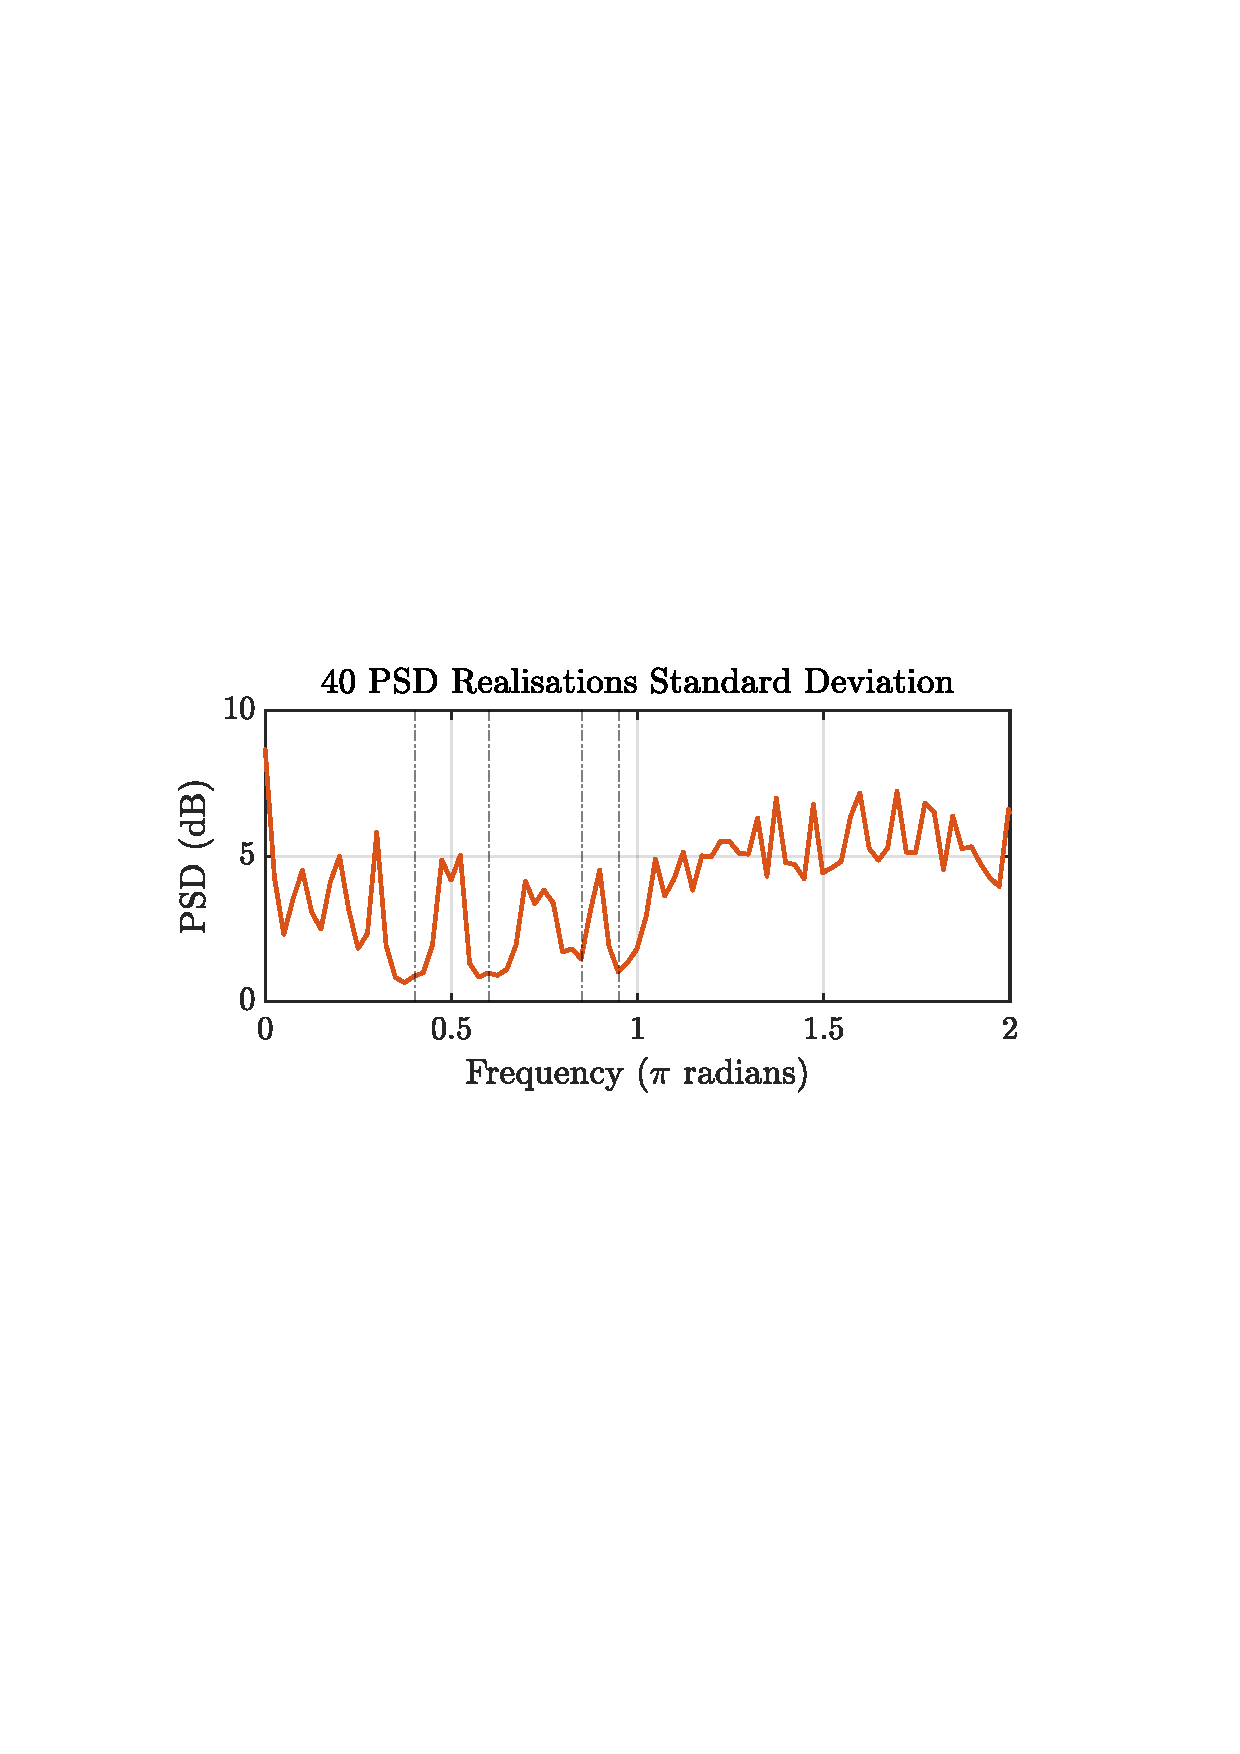
\includegraphics[trim={2.2cm 11.2cm 3.15cm  11.2cm}, clip, width=\textwidth]{../MATLAB/figures/q1_3c_fig02.pdf} 
			\captionsetup{justification=centering}
			\caption{Standard Deviation}
		\end{subfigure}
		\captionsetup{justification=centering}
		\caption{The total number of data points used was 512, black vertical lines indicate the model defined frequencies}
		\label{fig: 1-3c}
	\end{figure}

	Figure \ref{fig: 1-3c}. It is advantageous that the standard deviation decreases around our frequencies of interest instead of increases. 

	\subsubsection{Influence of Data Samples on the PSD}
	
	\begin{figure}[H]%{R}{0.49\textwidth}
%	\begin{figure}[H]
		\centering
			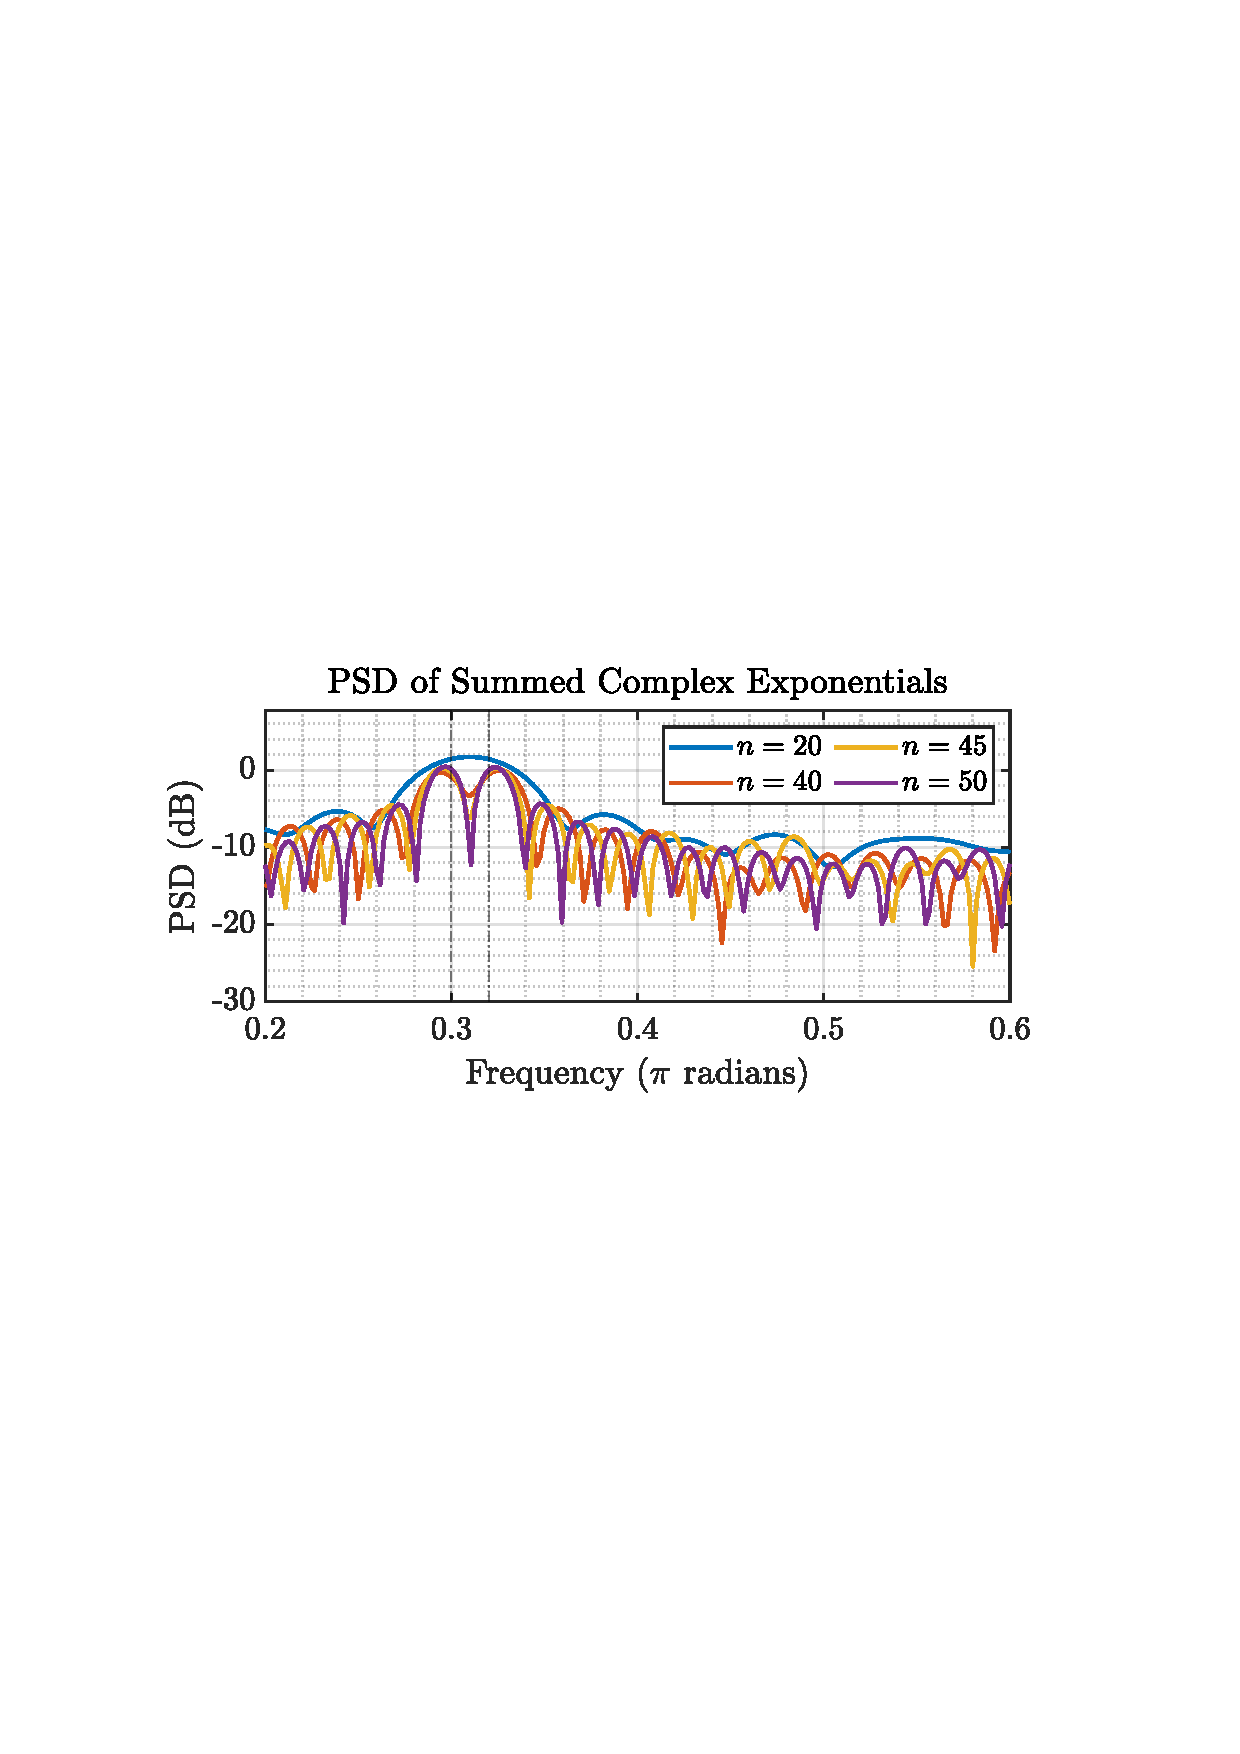
\includegraphics[trim={2.2cm 11.2cm 3.15cm  11.2cm}, clip, width=0.49\textwidth]{../MATLAB/figures/q1_3d_fig01.pdf} 
%		\end{centering}
%	\end{figure}
	\captionsetup{justification=centering}
	\caption{PSD while varying $n$, the number of Data Samples used}
	\label{fig: 1-3d}
	\end{figure}
	
	In Figure \ref{fig: 1-3d} we can clearly see that the frequency resolution is insufficient at lower sample numbers, resulting in aliasing of the desired frequency peaks.
	
	\subsubsection{MUltiple SIgnal Classification (MUSIC) Estimator}
	
	\begin{figure}[H]
		\centering
		\begin{subfigure}{0.49\textwidth}
			\centering
			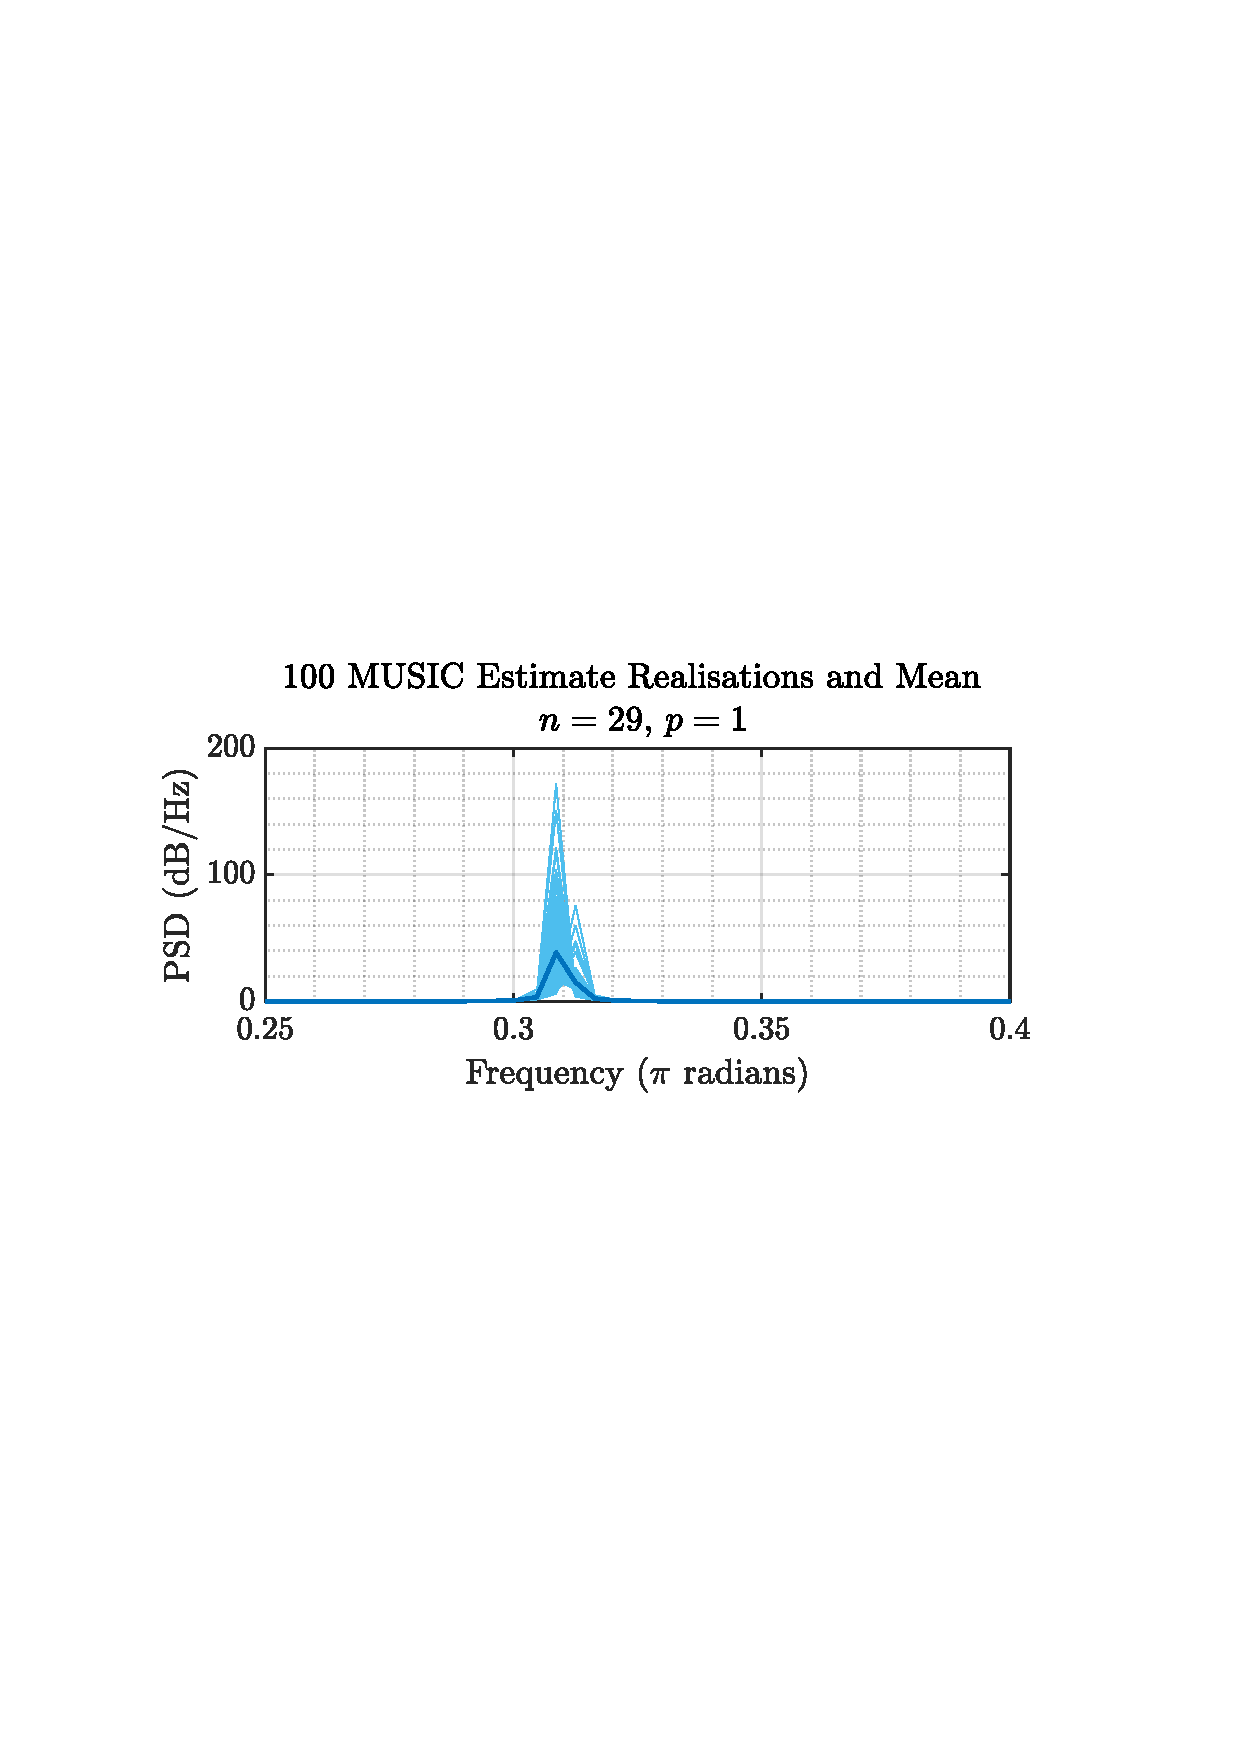
\includegraphics[trim={2.2cm 11cm 3.15cm  11.2cm}, clip, width=\textwidth]{../MATLAB/figures/q1_3e_fig01.pdf} 
		\end{subfigure}
		%		~ % forces onto the same row
		\begin{subfigure}{0.49\textwidth}
			\centering
			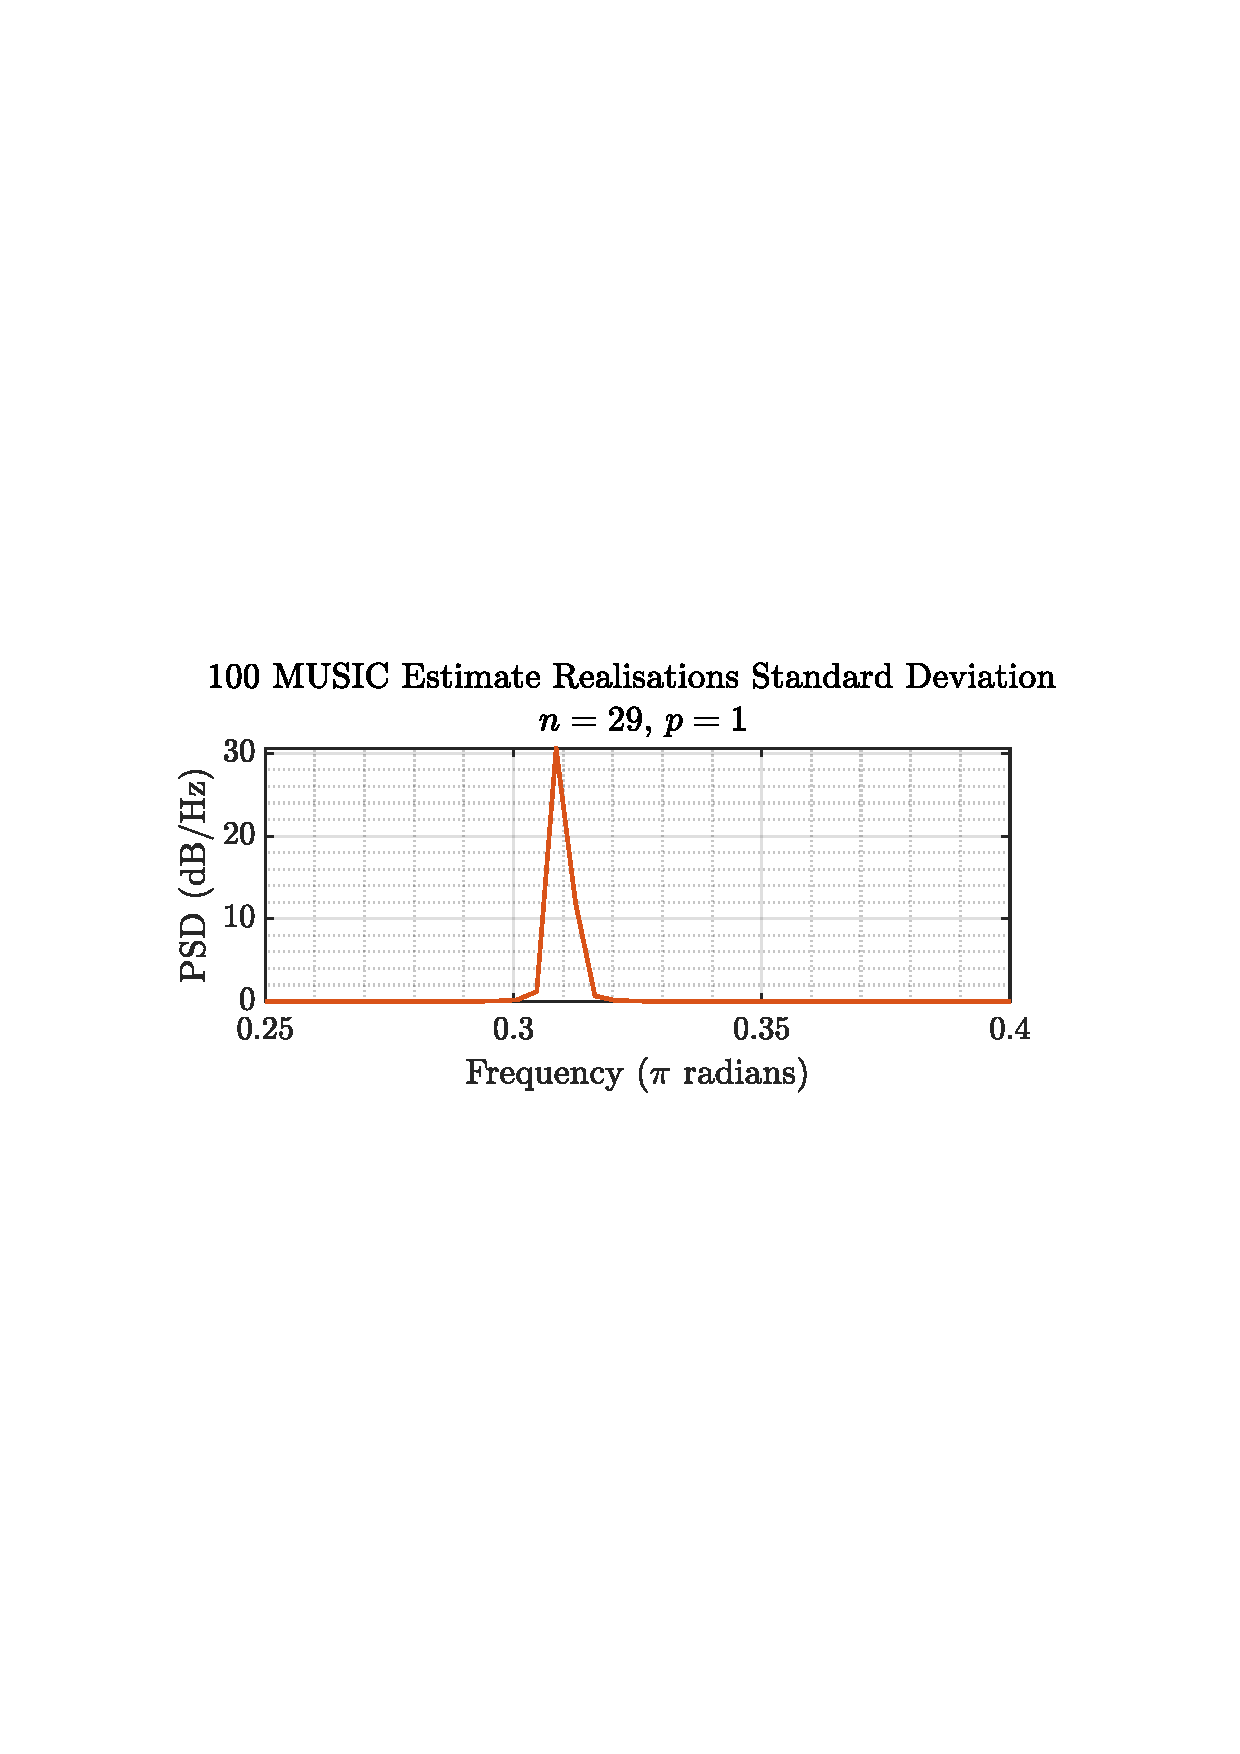
\includegraphics[trim={2.2cm 11cm 3.15cm  11.2cm}, clip, width=\textwidth]{../MATLAB/figures/q1_3e_fig02.pdf} 
		\end{subfigure}
		\begin{subfigure}{0.49\textwidth}
			\centering
			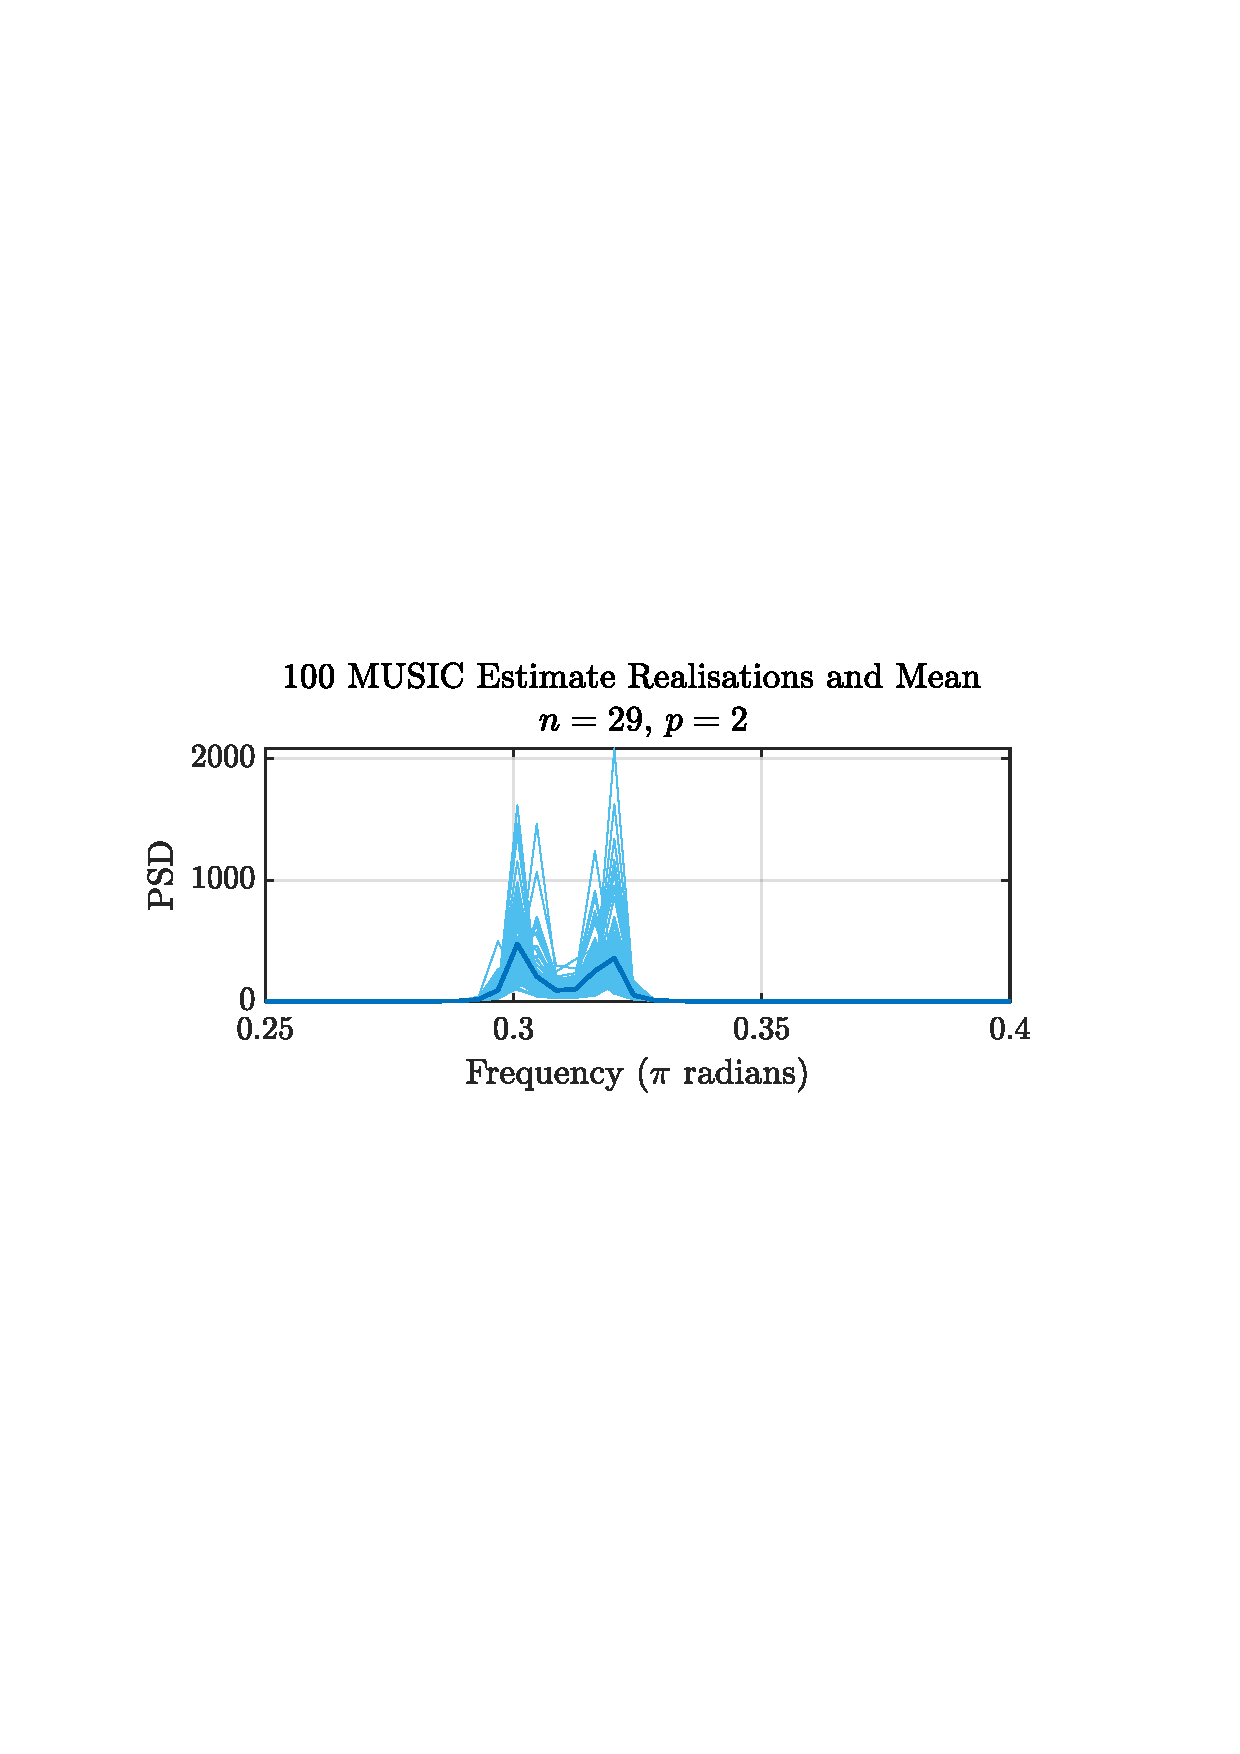
\includegraphics[trim={2.2cm 11cm 3.15cm  11.2cm}, clip, width=\textwidth]{../MATLAB/figures/q1_3e_fig03.pdf} 
		\end{subfigure}
		%		~ % forces onto the same row
		\begin{subfigure}{0.49\textwidth}
			\centering
			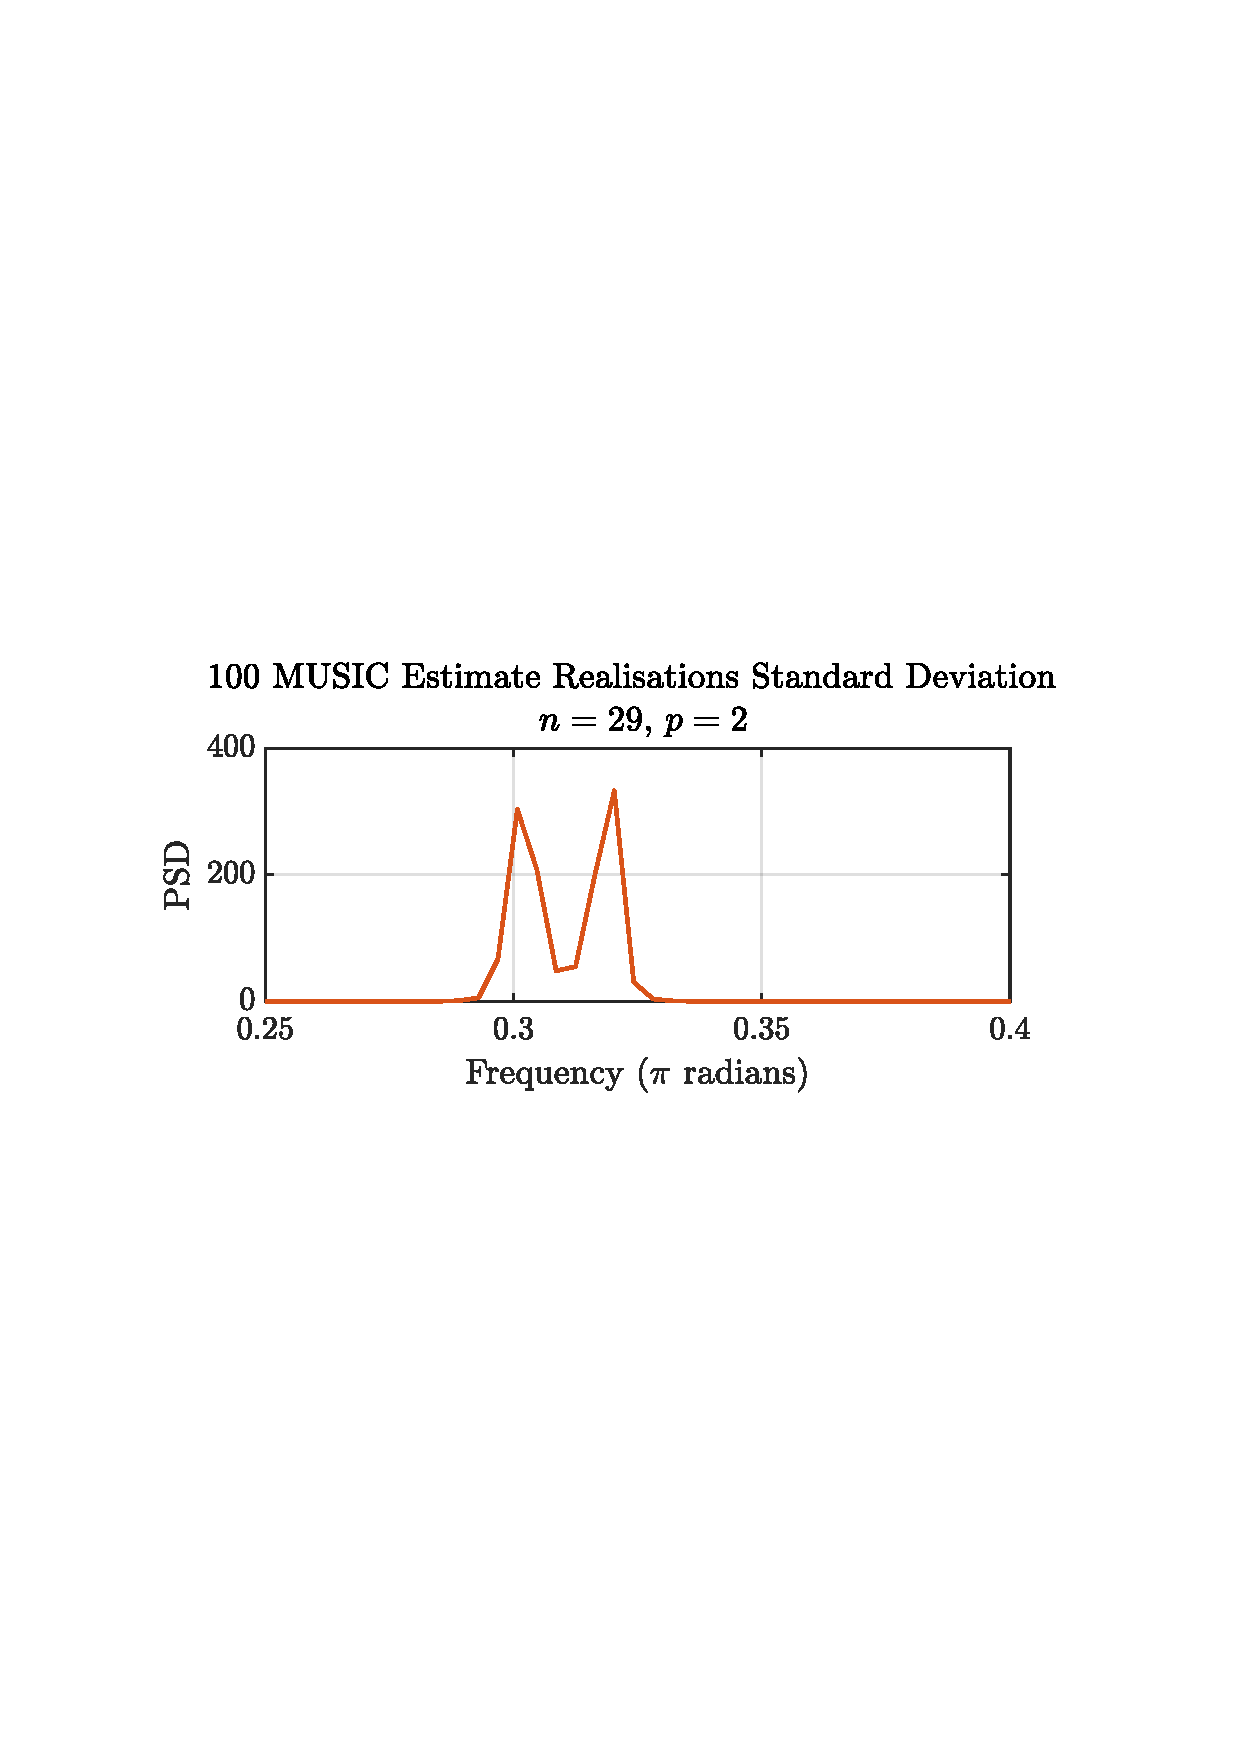
\includegraphics[trim={2.2cm 11cm 3.15cm  11.2cm}, clip, width=\textwidth]{../MATLAB/figures/q1_3e_fig04.pdf} 
		\end{subfigure}
		\begin{subfigure}{0.49\textwidth}
			\centering
			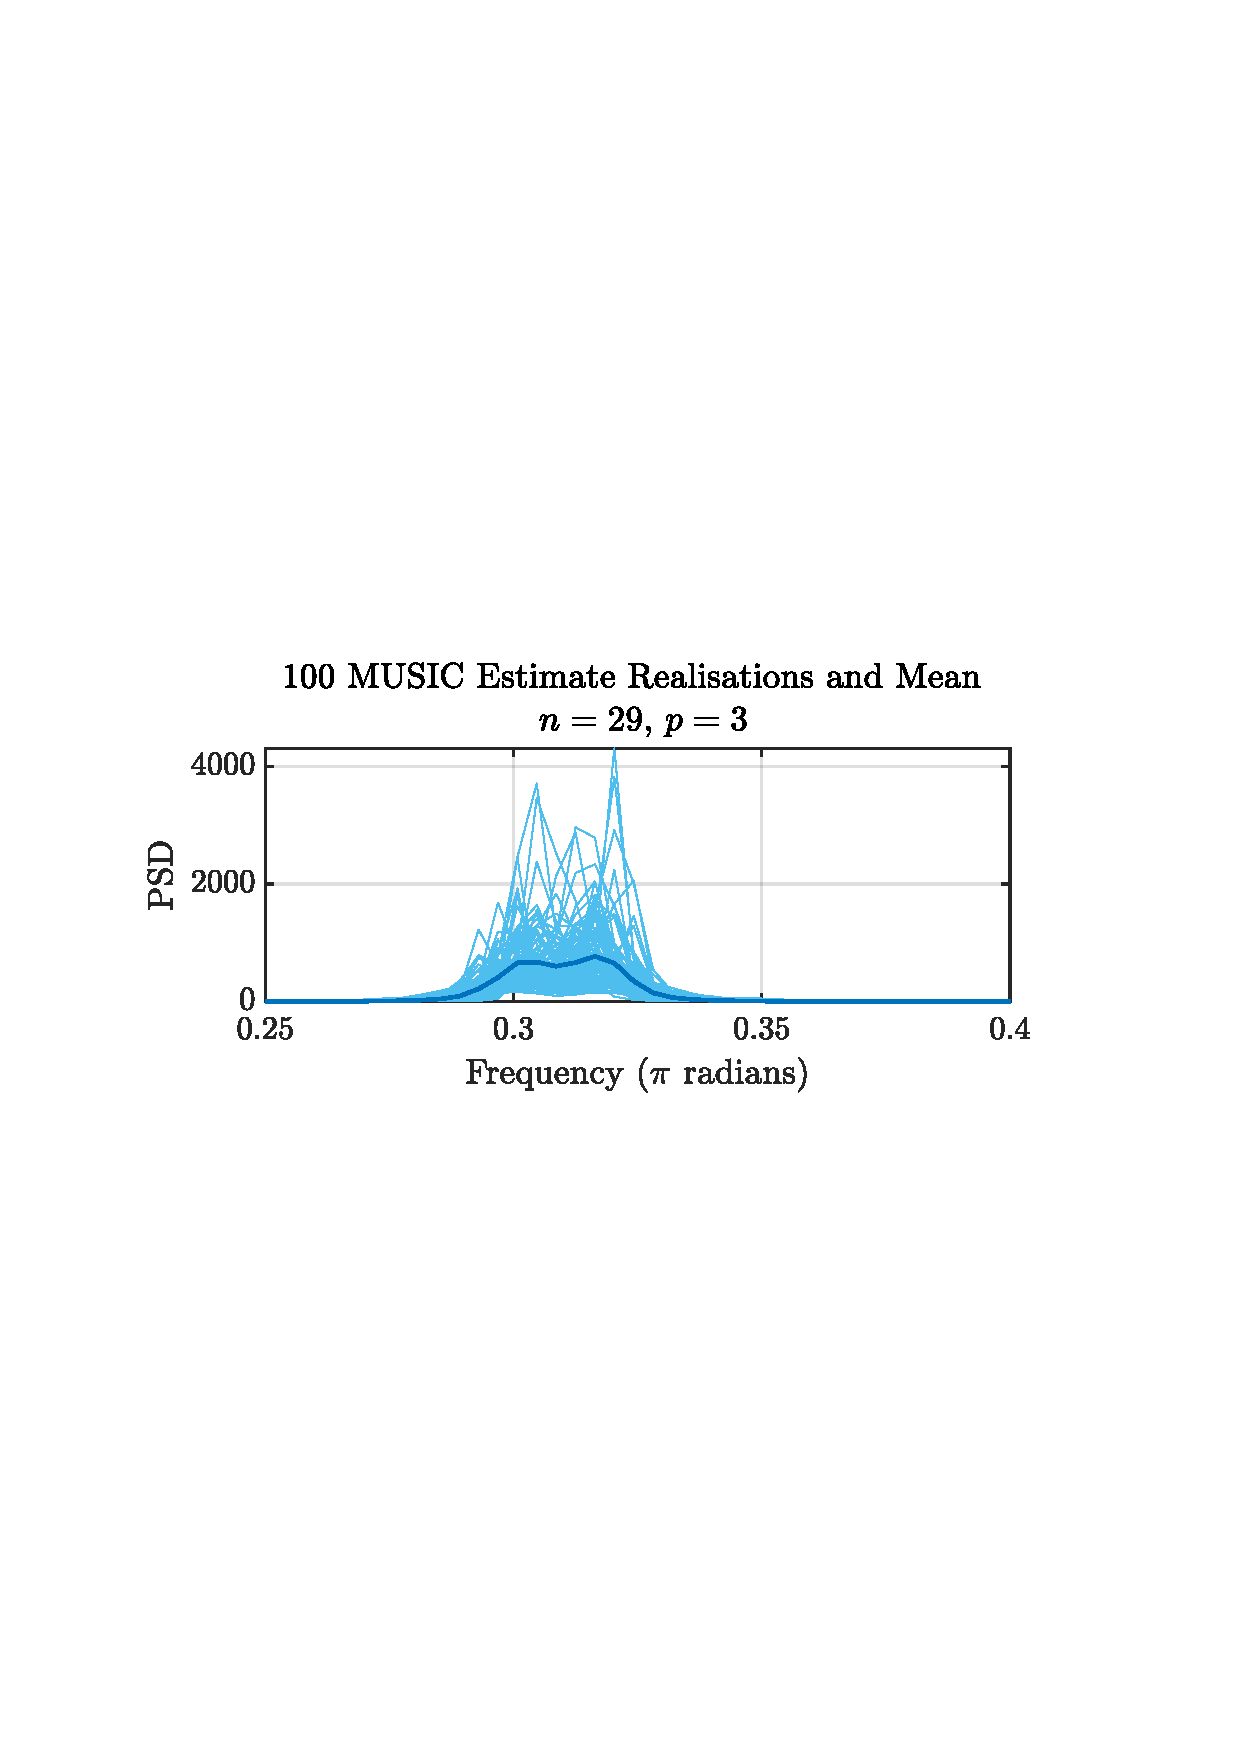
\includegraphics[trim={2.2cm 11.2cm 3.15cm  11.2cm}, clip, width=\textwidth]{../MATLAB/figures/q1_3e_fig05.pdf} 
		\end{subfigure}
		%		~ % forces onto the same row
		\begin{subfigure}{0.49\textwidth}
			\centering
			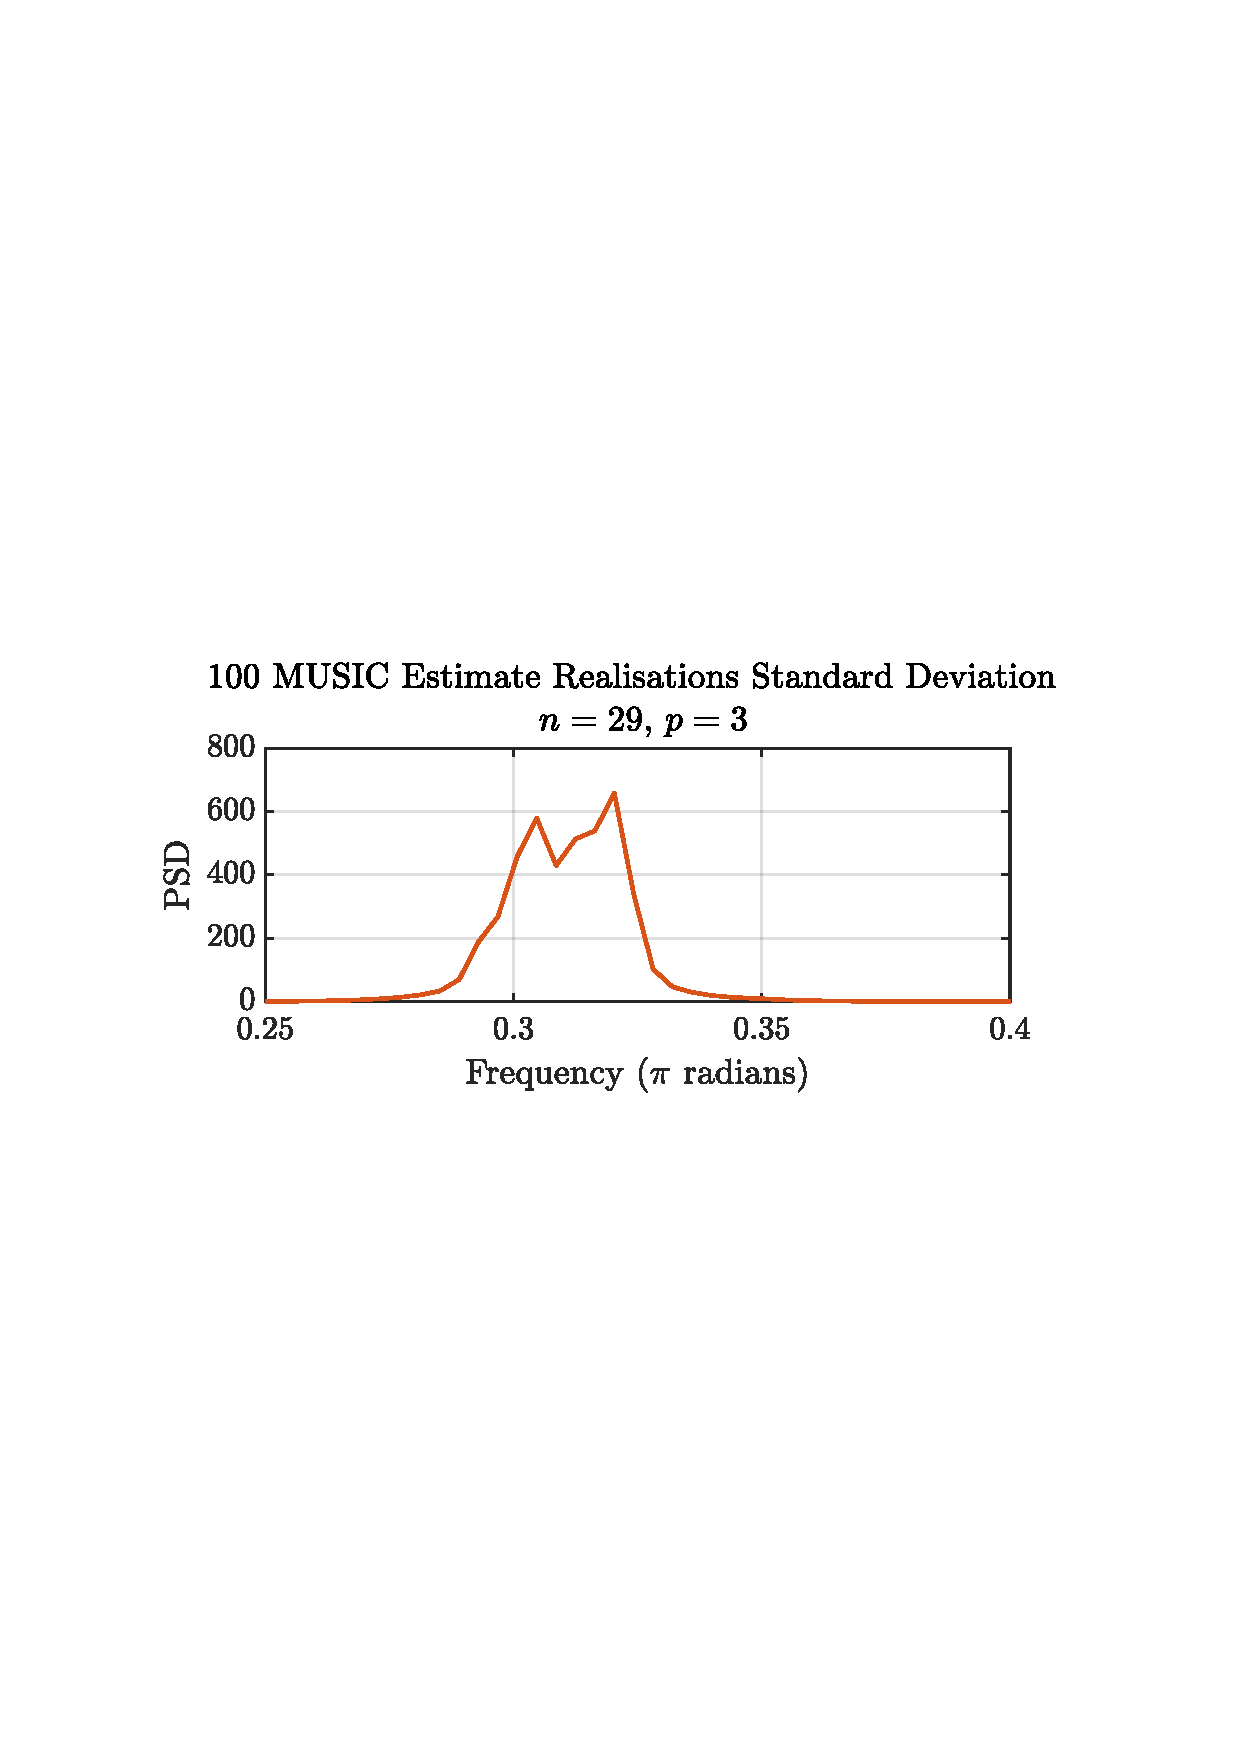
\includegraphics[trim={2.2cm 11.2cm 3.15cm  11.2cm}, clip, width=\textwidth]{../MATLAB/figures/q1_3e_fig06.pdf} 
		\end{subfigure}
		\captionsetup{justification=centering}
		\caption{Set of Auto-Correlation Functions (ACFs) and their Correlograms. \\ $n$ is the number of samples used, $p$ is the Signal Space Dimensionality}
		\label{fig: 1-3e}
	\end{figure}

	The MUSIC estimate identifies eigenvalues of an autocorrelation matrix in descending magnitude order - which indicate directions of largest variability in the subspace. \\
	The first line creates the 14 dimensional modified correlation matrix $R_{xx}$ for the dataset, which is subsequently used by the MUSIC algorithm with $p$ setting the Signal Subspace Dimensionality in the second line. \\
	The third line plots the Pseudospectrum (PSD Estimate) against the frequency axis. \\
	
	Figure \ref{fig: 1-3e} shows the MUSIC estimate plots for the given equation. The spectrum is not very detailed, peaks are not all sharp, but are clearly distinguishable from the surrounding periodogram. In the general case the MUSIC estimator is a good choice if the signal space dimensionality is known, especially as it works on such a limited set of samples. \\
	
	The periodogram is equally suitable for resolving peaks, but requires more samples for a meaningful resolution. \\
	
	In both periodogram and MUSIC estimators we see that the standard deviation, hence variance increase around the peaks, except when using the log scale of the periodogram, where it decreases.
	
	% TODO: A figure doing a direct comparison for the same signal maybe.
	
	% TODO: Bias and Variance
	
	\subsection{Spectrum of Autoregressive (AR) Processes} \label{sec: 1-4-spectrums-AR}

	
	\subsubsection{Shortcomings of the Unbiased ACF in finding AR Parameters}
	
	As the unbiased estimator allows for negative values, at a computational level it will require more bits to store, especially for larger values.
	
	\subsubsection{Error of the AR PSD Estimate}
	\begin{figure}[H]
		\centering
		\begin{subfigure}{0.49\textwidth}
			\centering
			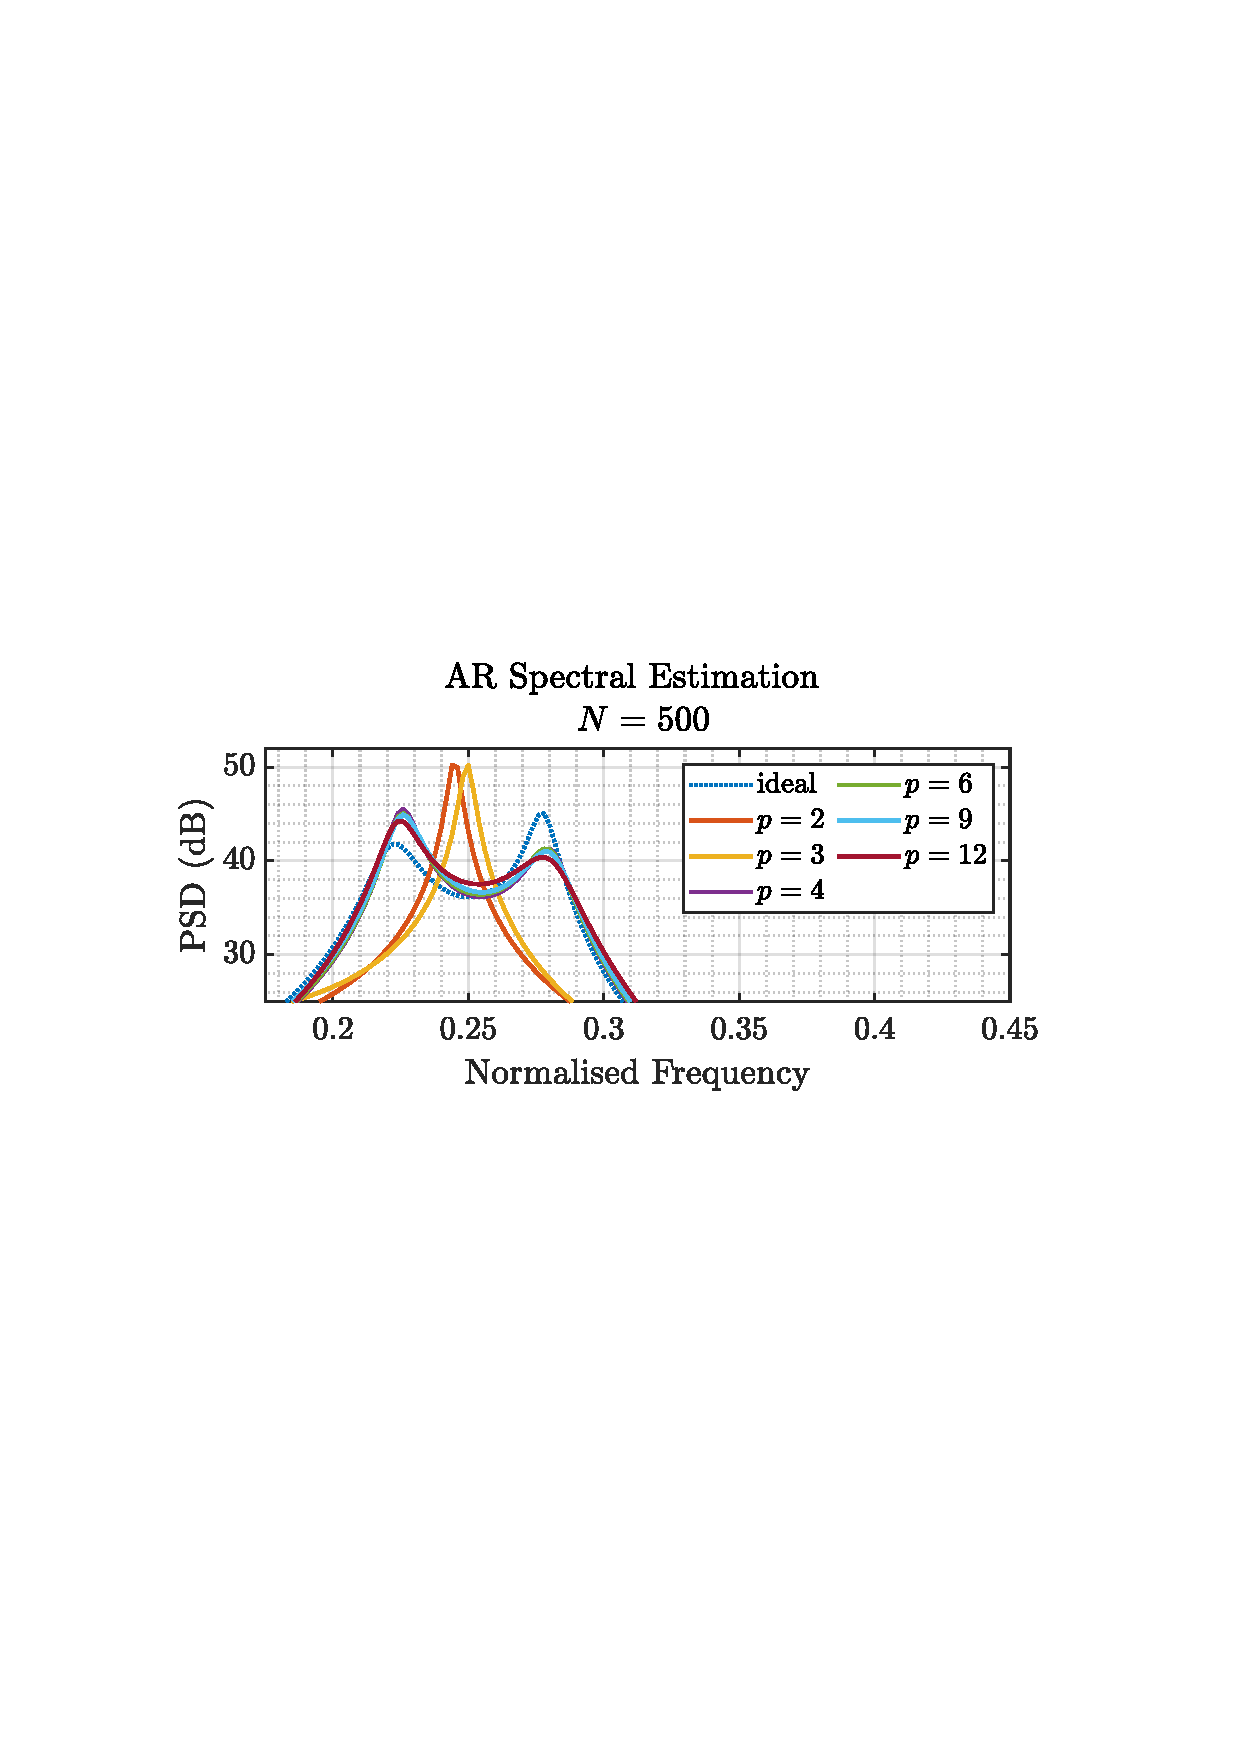
\includegraphics[trim={2.2cm 11.2cm 3.15cm  11.2cm}, clip, width=\textwidth]{../MATLAB/figures/q1_4b_fig14.pdf} 
			\captionsetup{justification=centering}
			\caption{AR Periodogram and its $p$ Order Estimates}
		\end{subfigure}
		%		~ % forces onto the same row
		\begin{subfigure}{0.49\textwidth}
			\centering
			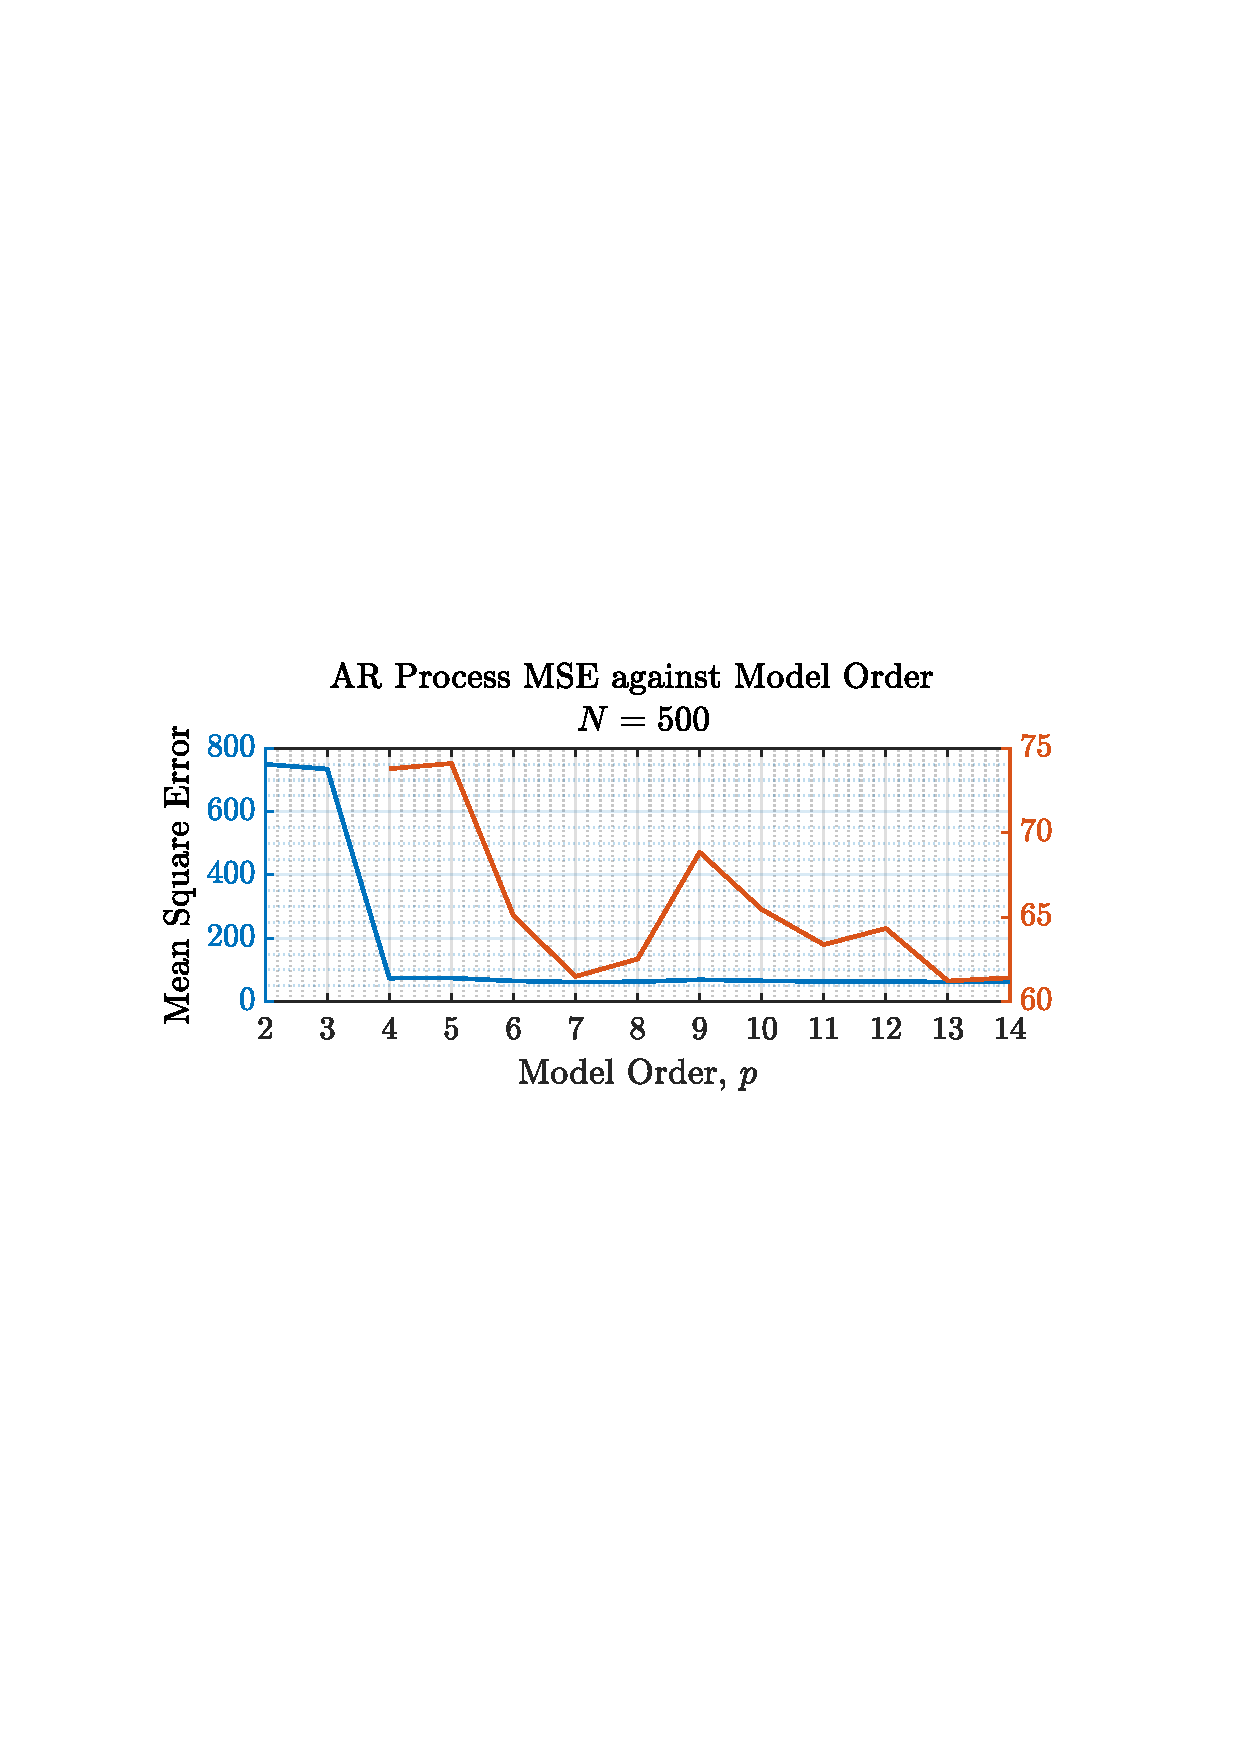
\includegraphics[trim={2.2cm 11.2cm 3.15cm  11.2cm}, clip, width=\textwidth]{../MATLAB/figures/q1_4b_fig16.pdf} 
			\captionsetup{justification=centering}
			\caption{Mean Squared Error with two y-scales}
		\end{subfigure}
		\captionsetup{justification=centering}
		\caption{}
		\label{fig: 1-4b}
	\end{figure}

	We can see in (a) of \ref{fig: 1-4b}, that increasing the order tends towards a better solution. But (b) notes that the most drastic difference is at the model order, 4, which matches the order of the process defined, subsequent increases of the model order do increase its likeliness to the true response, but changes are not so drastic.
	

	\subsubsection{Error of the AR PSD Estimate with more Samples}
	\begin{figure}[H]
		\centering
		\begin{subfigure}{0.49\textwidth}
			\centering
			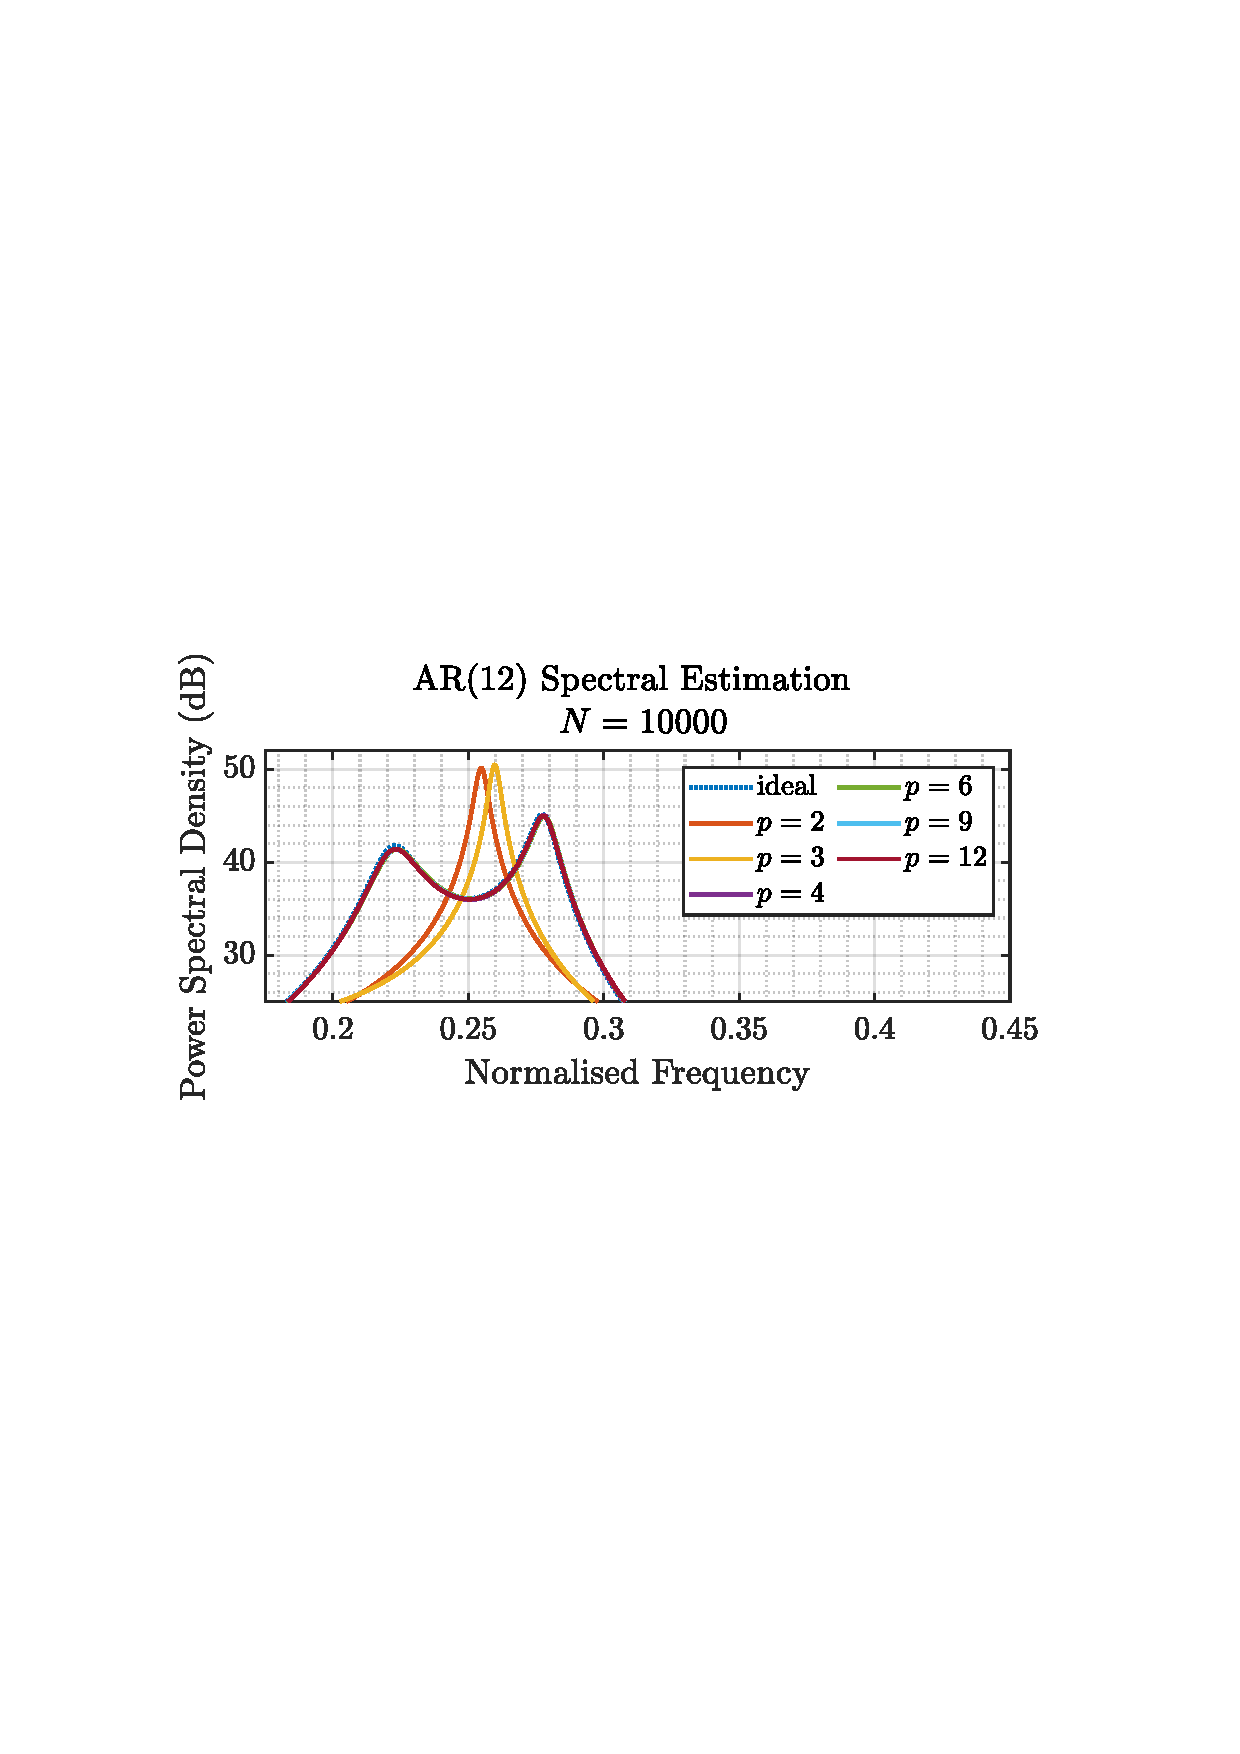
\includegraphics[trim={2.2cm 11.2cm 3.15cm  11.2cm}, clip, width=\textwidth]{../MATLAB/figures/q1_4c_fig14.pdf} 
			\captionsetup{justification=centering}
			\caption{AR Periodogram and its $p$ Order Estimates}
		\end{subfigure}
		%		~ % forces onto the same row
		\begin{subfigure}{0.49\textwidth}
			\centering
			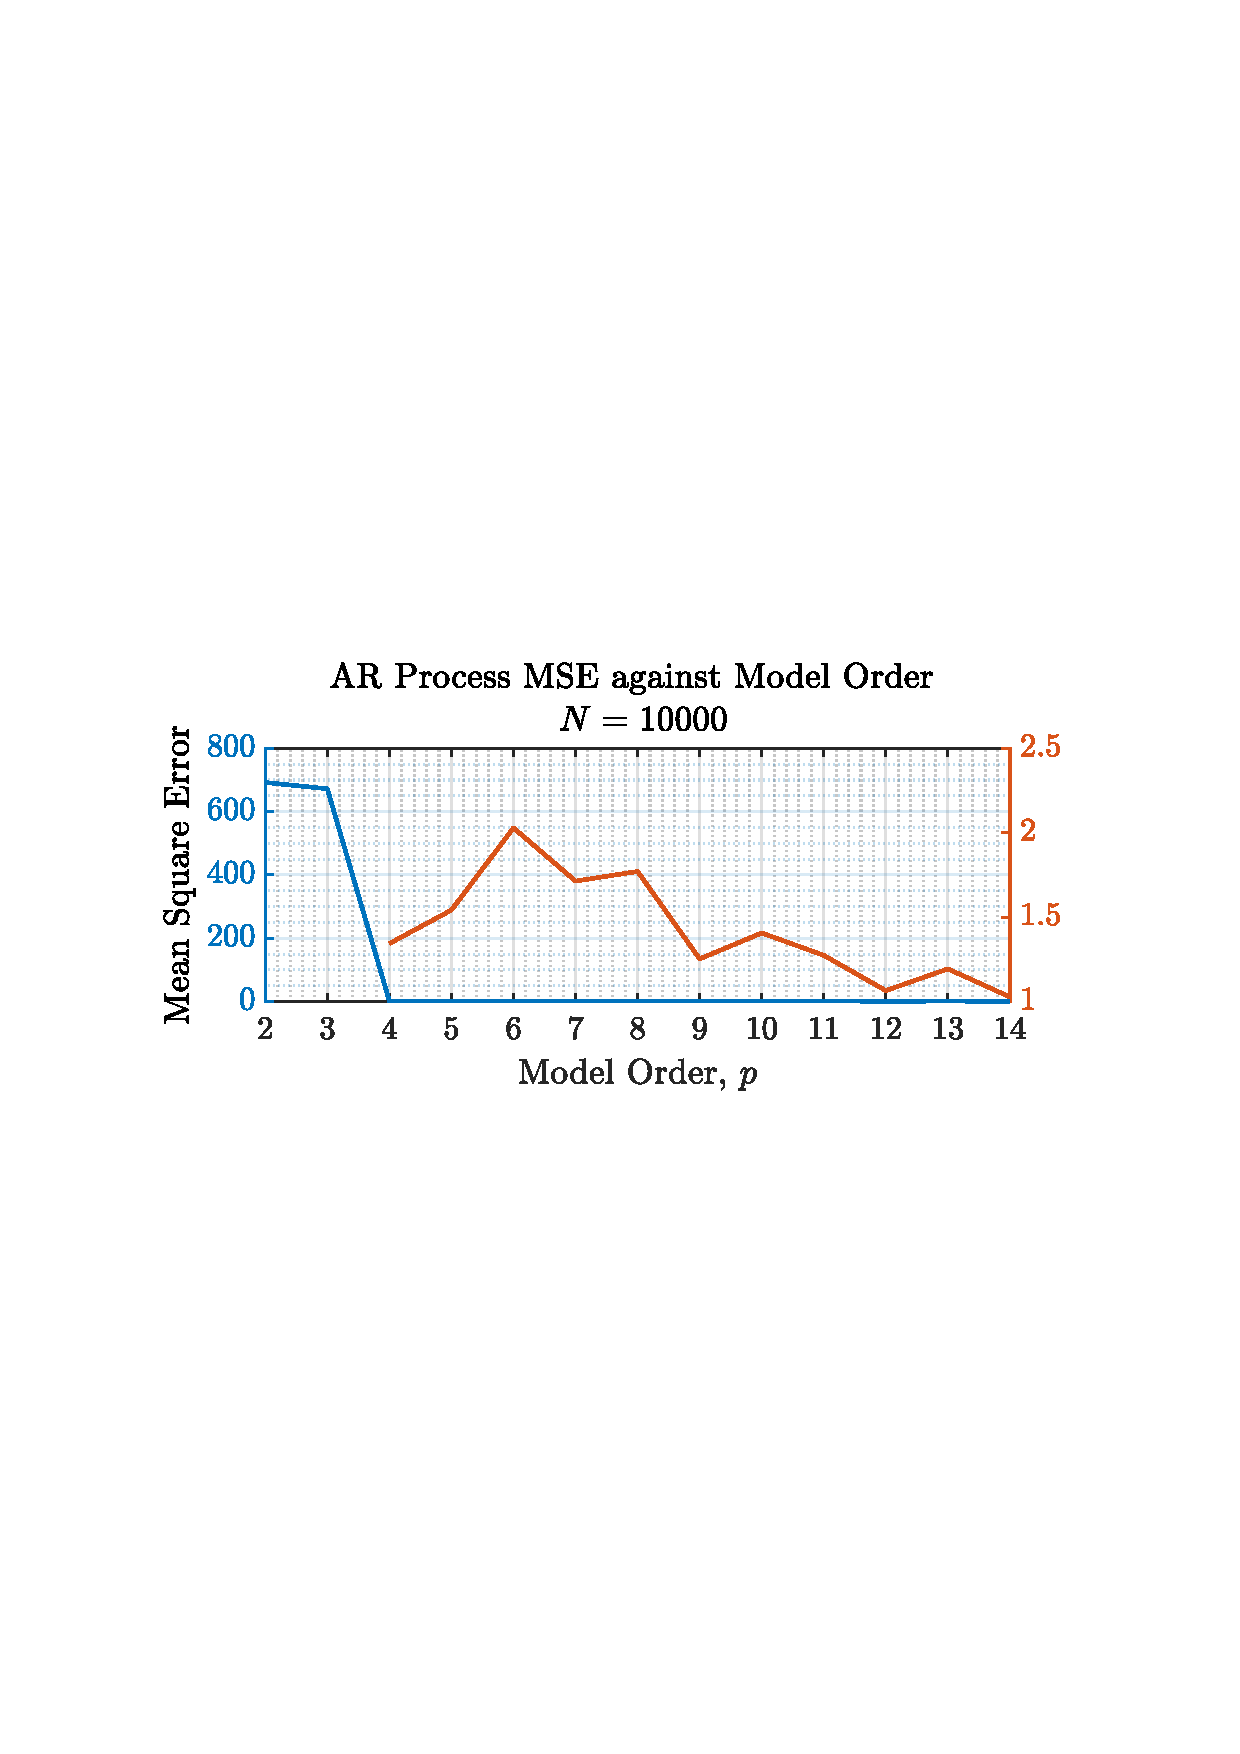
\includegraphics[trim={2.2cm 11.2cm 3cm  11.2cm}, clip, width=\textwidth]{../MATLAB/figures/q1_4c_fig16.pdf} 
			\captionsetup{justification=centering}
			\caption{Mean Squared Error with two y-scales}
		\end{subfigure}
		\captionsetup{justification=centering}
		\caption{}
		\label{fig: 1-4c}
	\end{figure}

	The same trend is seen in Figure \ref{fig: 1-4c}, as we saw with $N=500$, although the estimate now matches the underlying model much better, reflected in the drastically lower MSE. \\
	
	It is noted that for a more valid comparison of model order's influence on the estimate's error the Akaike Information Criterion (AIC) or the Bayesian Information Criterion (BIC) are more suitable quantifiers of model order suitability than MSE. But the accuracy trend reflected in the MSE is still valid for our comparisons.
	
	\pagebreak
	
	\subsection{Real World Signals: Respiratory Sinus Arrhythmia from RR-Intervals} \label{sec: 1-5-real-world-signals}
	
	\subsubsection{Standard \& Average PSDs of the RRI Dataset}
	\begin{figure}[H]
		\centering
		\begin{subfigure}{0.49\textwidth}
			\centering
			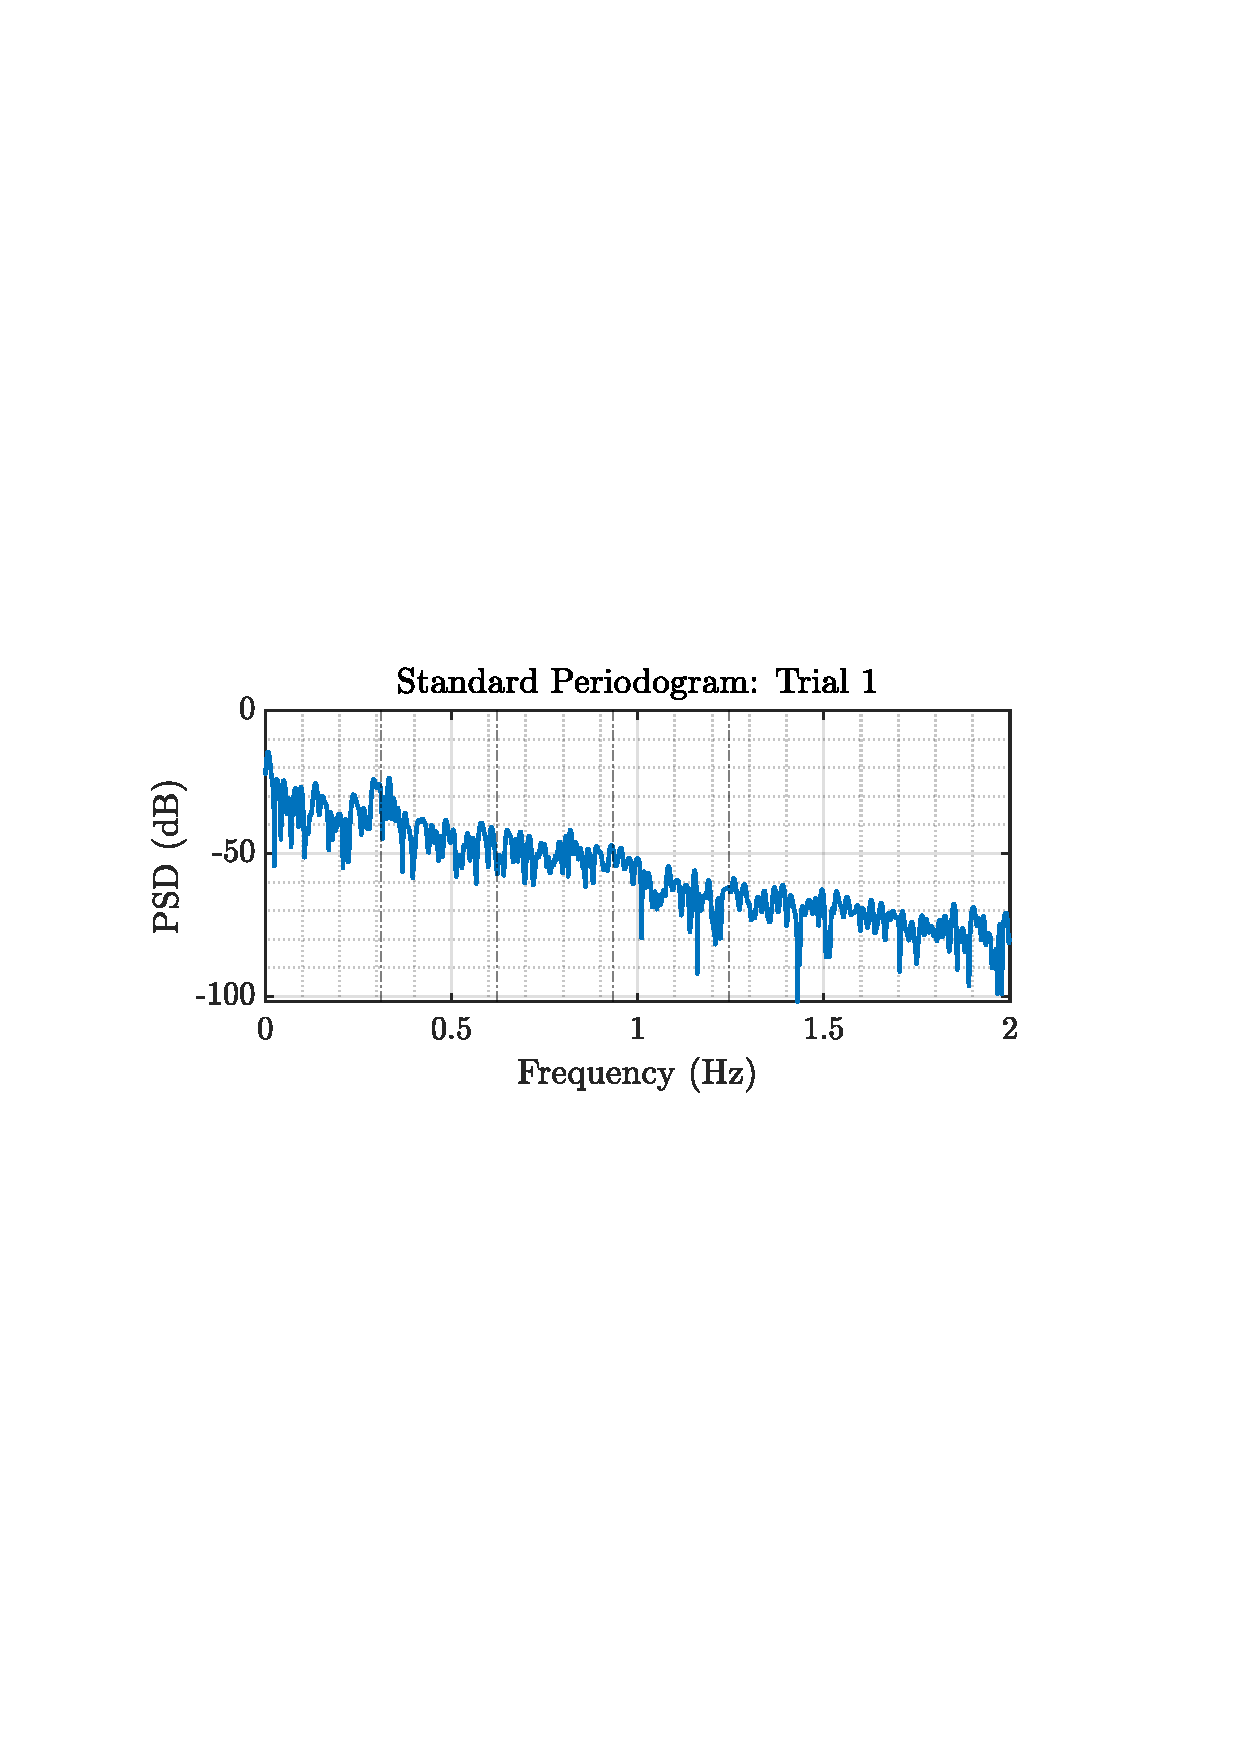
\includegraphics[trim={2.2cm 11cm 3.15cm  11.2cm}, clip, width=\textwidth]{../MATLAB/figures/q1_5a_fig01.pdf} 
		\end{subfigure}
		%		~ % forces onto the same row
		\begin{subfigure}{0.49\textwidth}
			\centering
			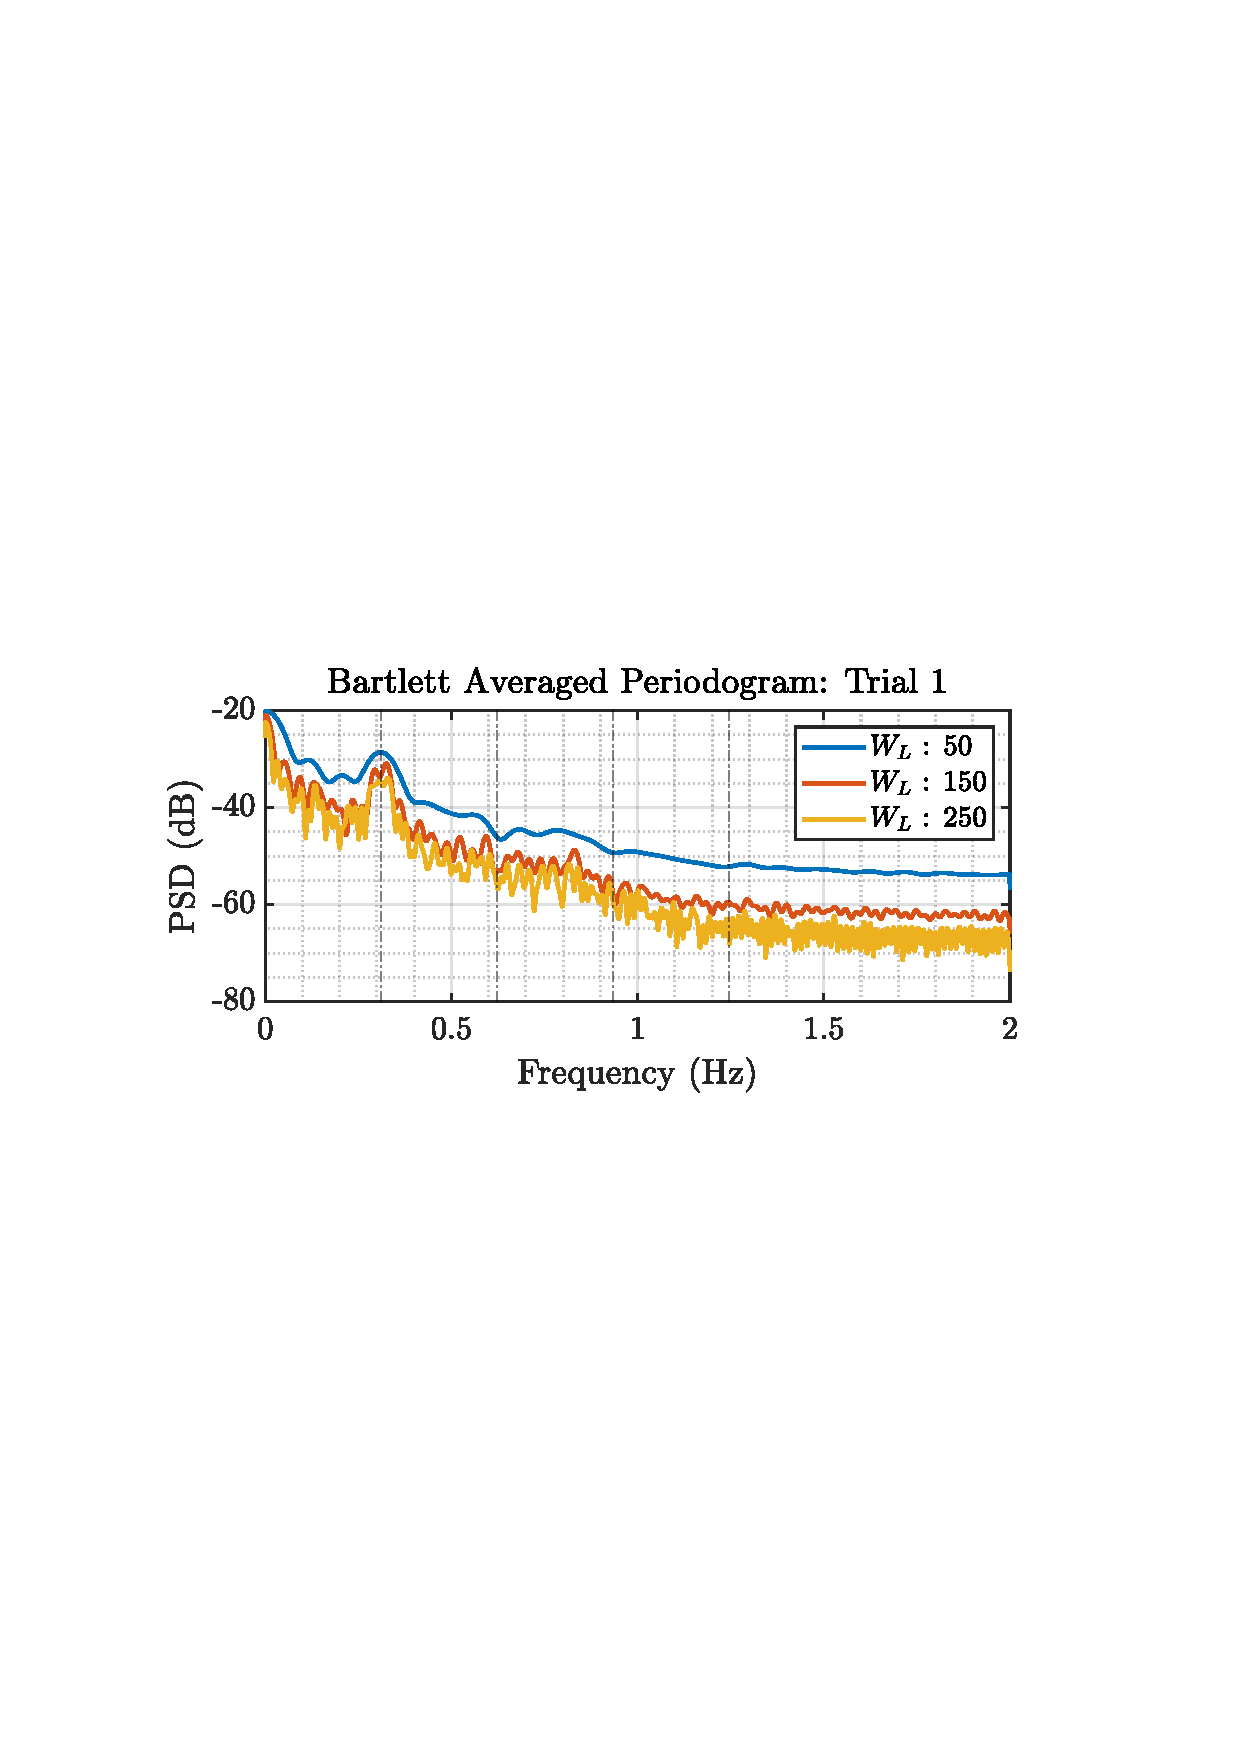
\includegraphics[trim={2.2cm 11cm 3.15cm  11.2cm}, clip, width=\textwidth]{../MATLAB/figures/q1_5a_fig04.pdf} 
		\end{subfigure}
		\begin{subfigure}{0.49\textwidth}
			\centering
			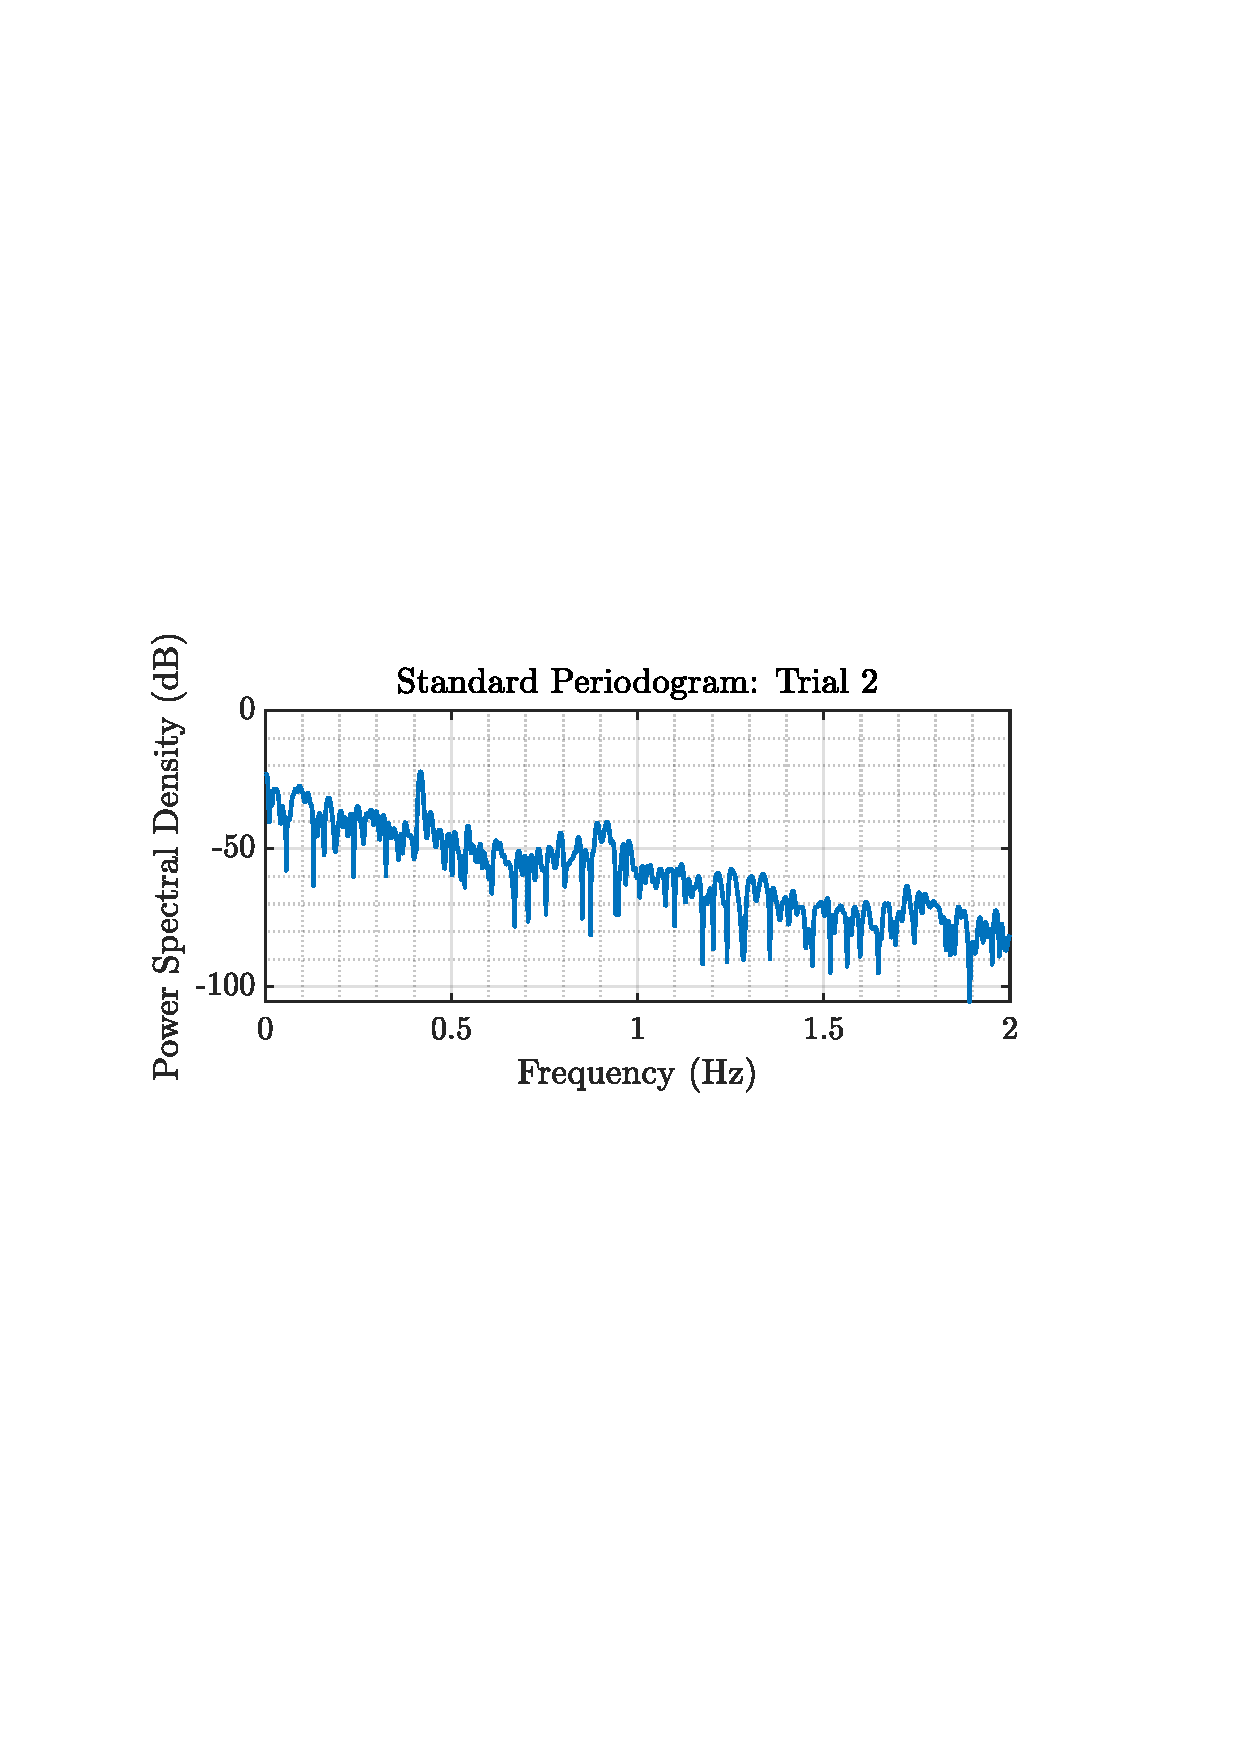
\includegraphics[trim={2.2cm 11cm 3.15cm  11.2cm}, clip, width=\textwidth]{../MATLAB/figures/q1_5a_fig02.pdf} 
		\end{subfigure}
		%		~ % forces onto the same row
		\begin{subfigure}{0.49\textwidth}
			\centering
			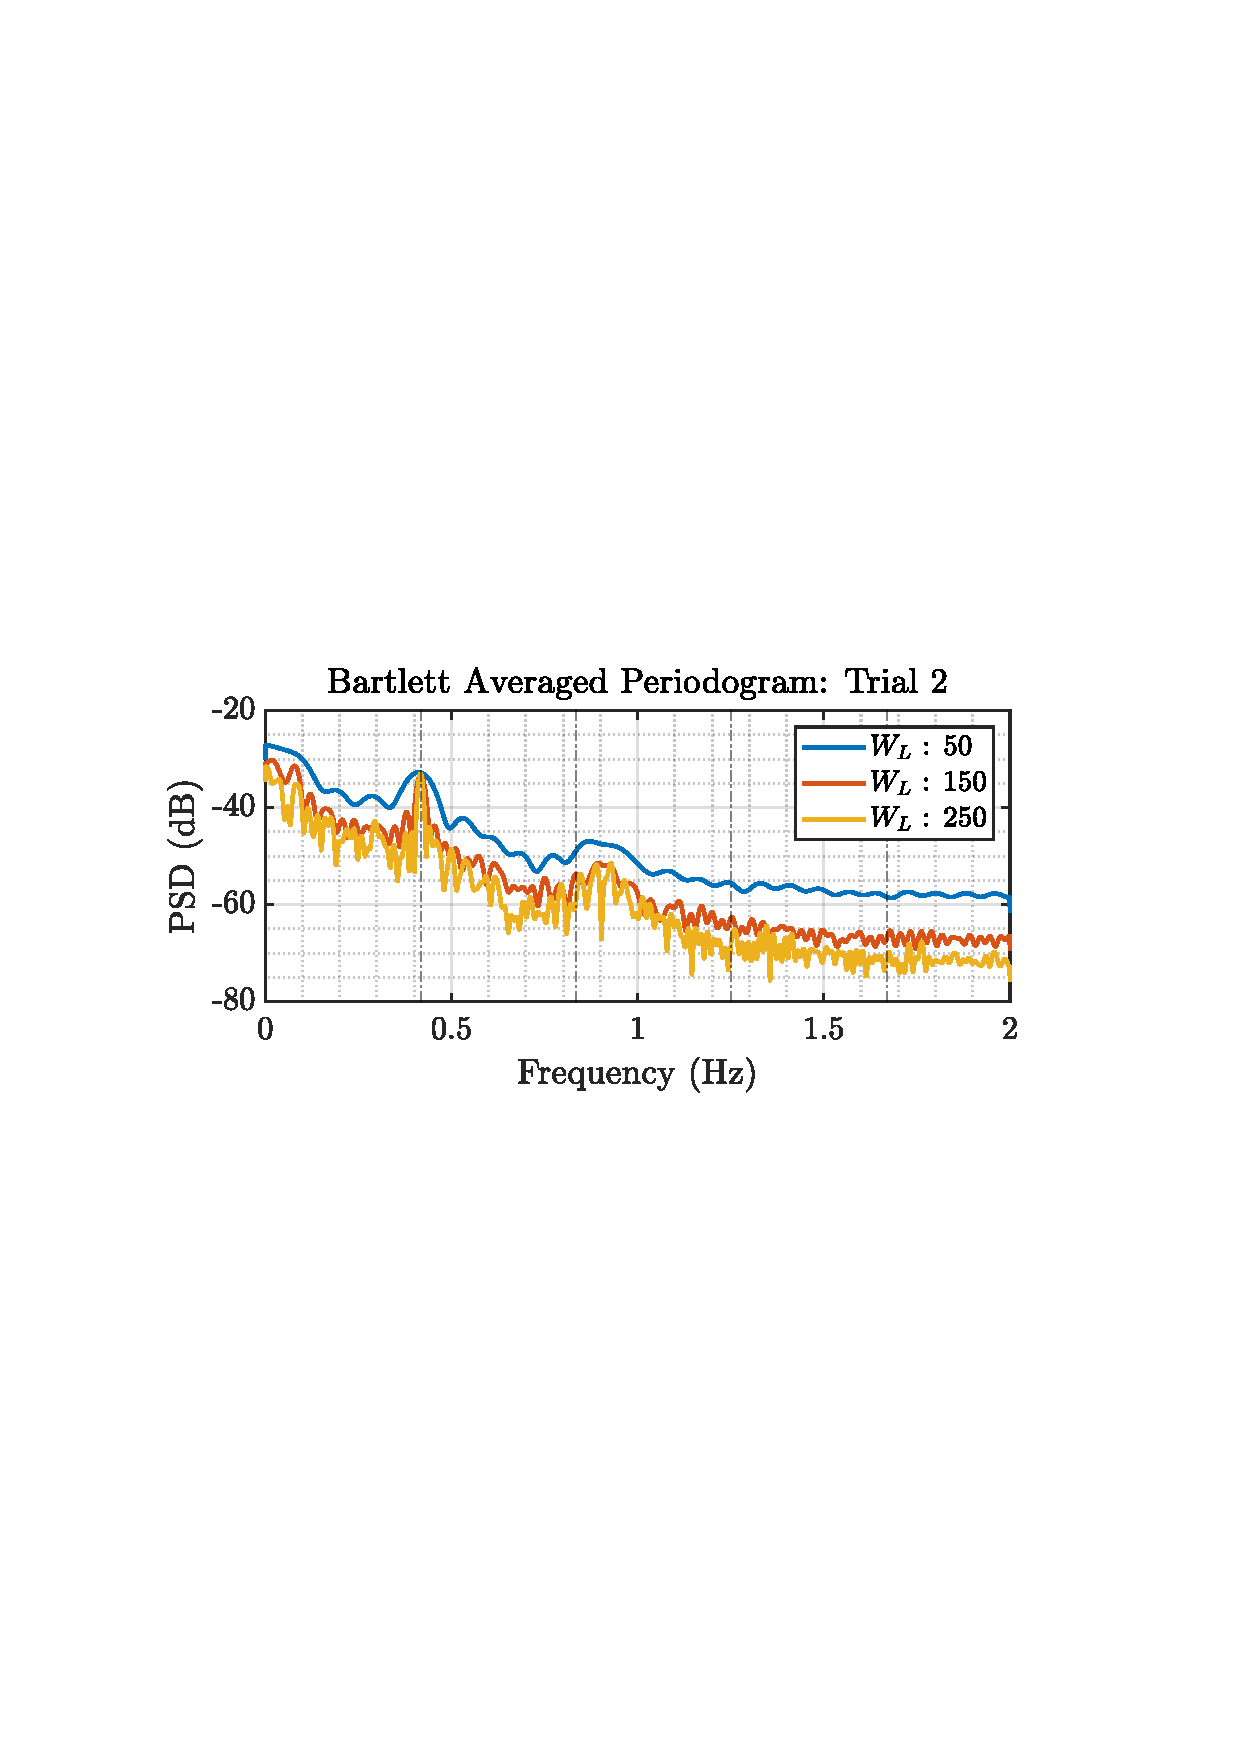
\includegraphics[trim={2.2cm 11cm 3.15cm  11.2cm}, clip, width=\textwidth]{../MATLAB/figures/q1_5a_fig05.pdf} 
		\end{subfigure}
		\begin{subfigure}{0.49\textwidth}
			\centering
			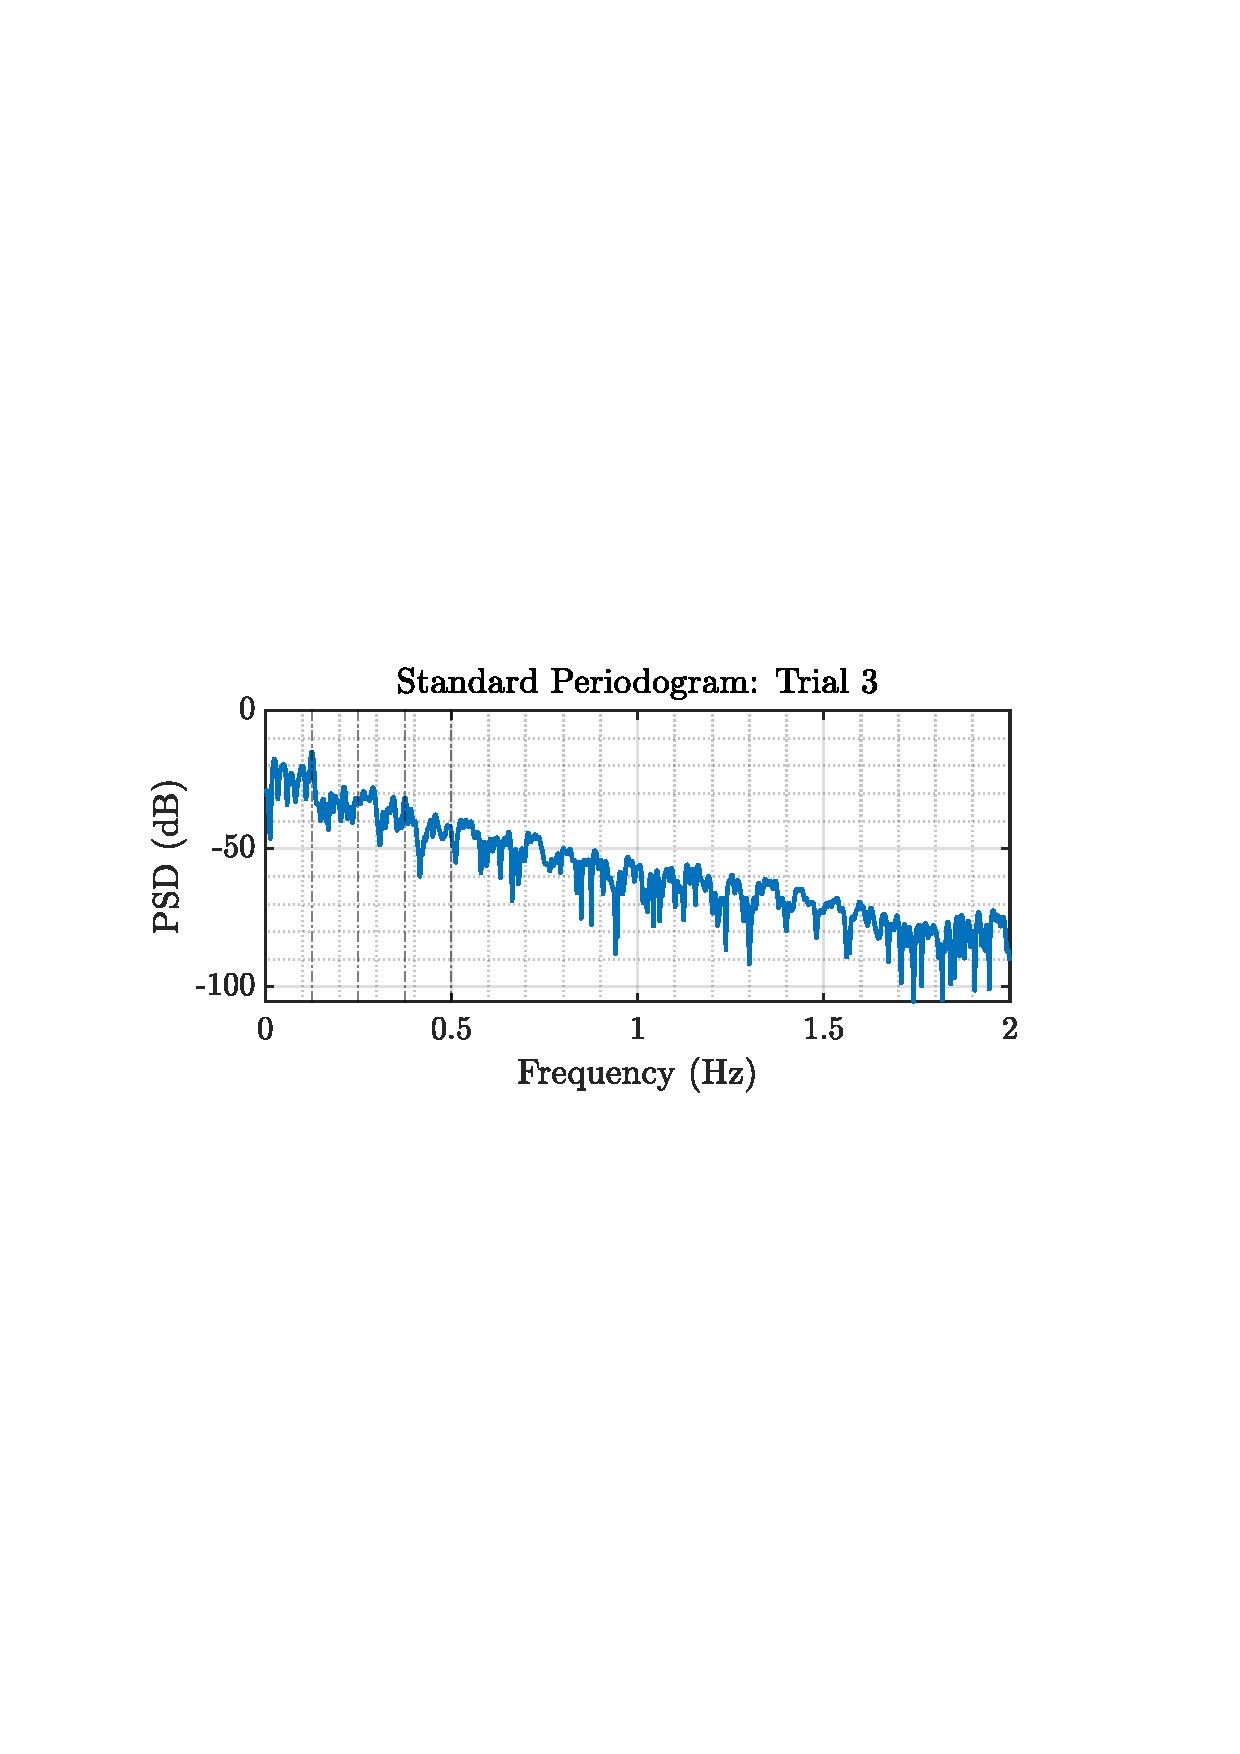
\includegraphics[trim={2.2cm 11.2cm 3.15cm  11.2cm}, clip, width=\textwidth]{../MATLAB/figures/q1_5a_fig03.pdf} 
		\end{subfigure}
		%		~ % forces onto the same row
		\begin{subfigure}{0.49\textwidth}
			\centering
			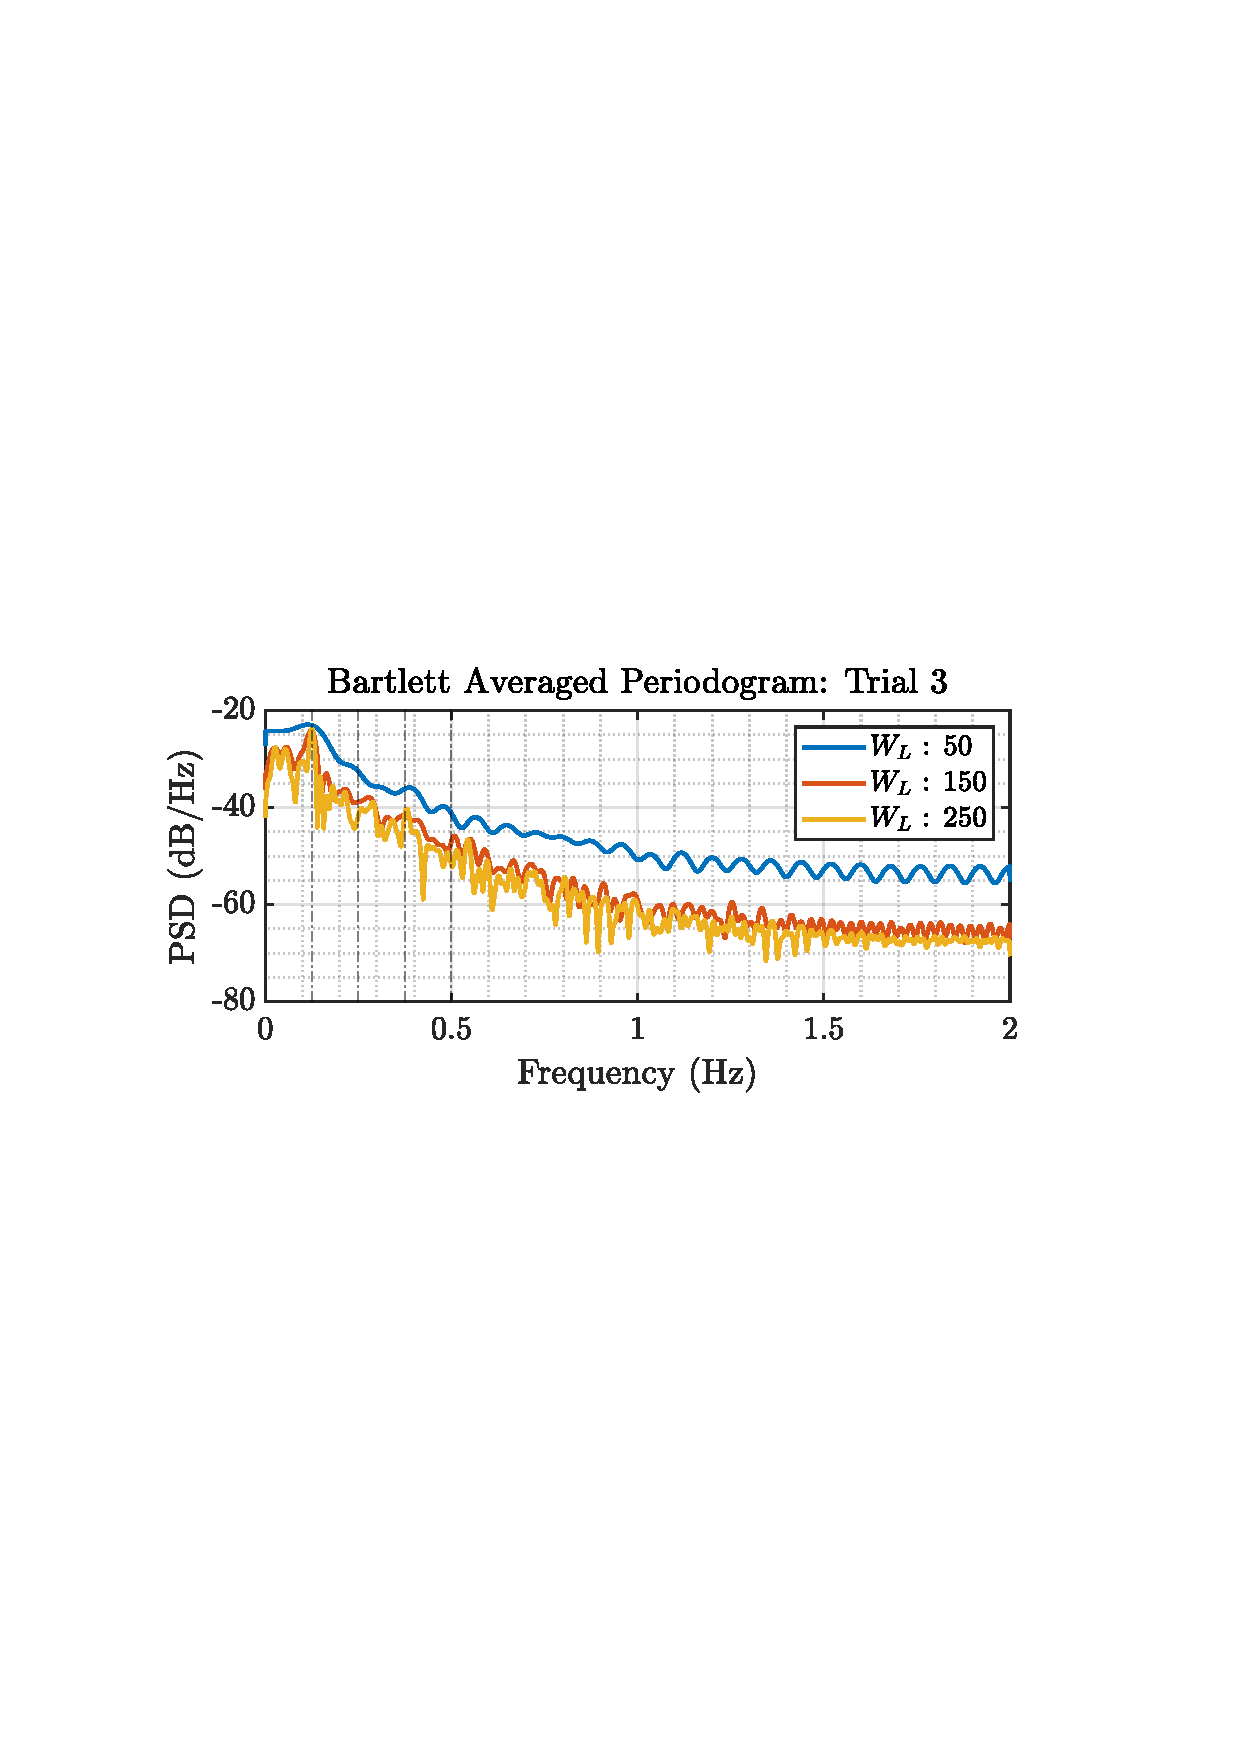
\includegraphics[trim={2.2cm 11.2cm 3.15cm  11.2cm}, clip, width=\textwidth]{../MATLAB/figures/q1_5a_fig06.pdf} 
		\end{subfigure}
		\captionsetup{justification=centering}
		\caption{Standard and Bartlett Average Periodograms. \\ 
				$W_L$ is the Window Length used. First 4 harmonics denoted by vertical black lines. Zero Padded Signal Length: $4096$.}
		\label{fig: 1-5a}
	\end{figure}

	\begin{table}[H]
		\centering
		\begin{tabular}{|c|c||c|}
			\hline
			\textbf{Breathing Type} & \textbf{Expected} (BPM) & \textbf{Observed Peak} (BPM) \\
			\hline
			\hline
			{Normal (Trial 1)} & $10-15$ & $0.31\times60\approx18.7$ \\
			\hline
			{Fast (Trial 2)} & $25$ & $0.41\times60\approx25$ \\
			\hline
			{Slow (Trial 3)} & $7.5$ & $0.125\times60=7.5$ \\
			\hline
		\end{tabular}
		\captionsetup{justification=centering}
		\caption{Breaths Per Minute (BPM), i.e. Observed Frequency $\times 60$, for all trials.}
		\label{tab: 1-5a}
	\end{table}


	\subsubsection{Analysis of the RRI PSD Estimates}
	
	Figure \ref{fig: 1-5a} shows us distinct peaks for each trial that somewhat agrees with the breathing expected. We note that harmonics are difficult to distinguish, despite the large zero padding of the signal. Table \ref{tab: 1-5a} highlights how the observed peaks align with the expected peaks.
	\pagebreak
	
	\subsubsection{AR PSD Estimate for the RRI Dataset}
	
%	\begin{wrapfigure}{r}{0.49\textwidth}
%		\vspace{-20pt}
%		\begin{centering}
%			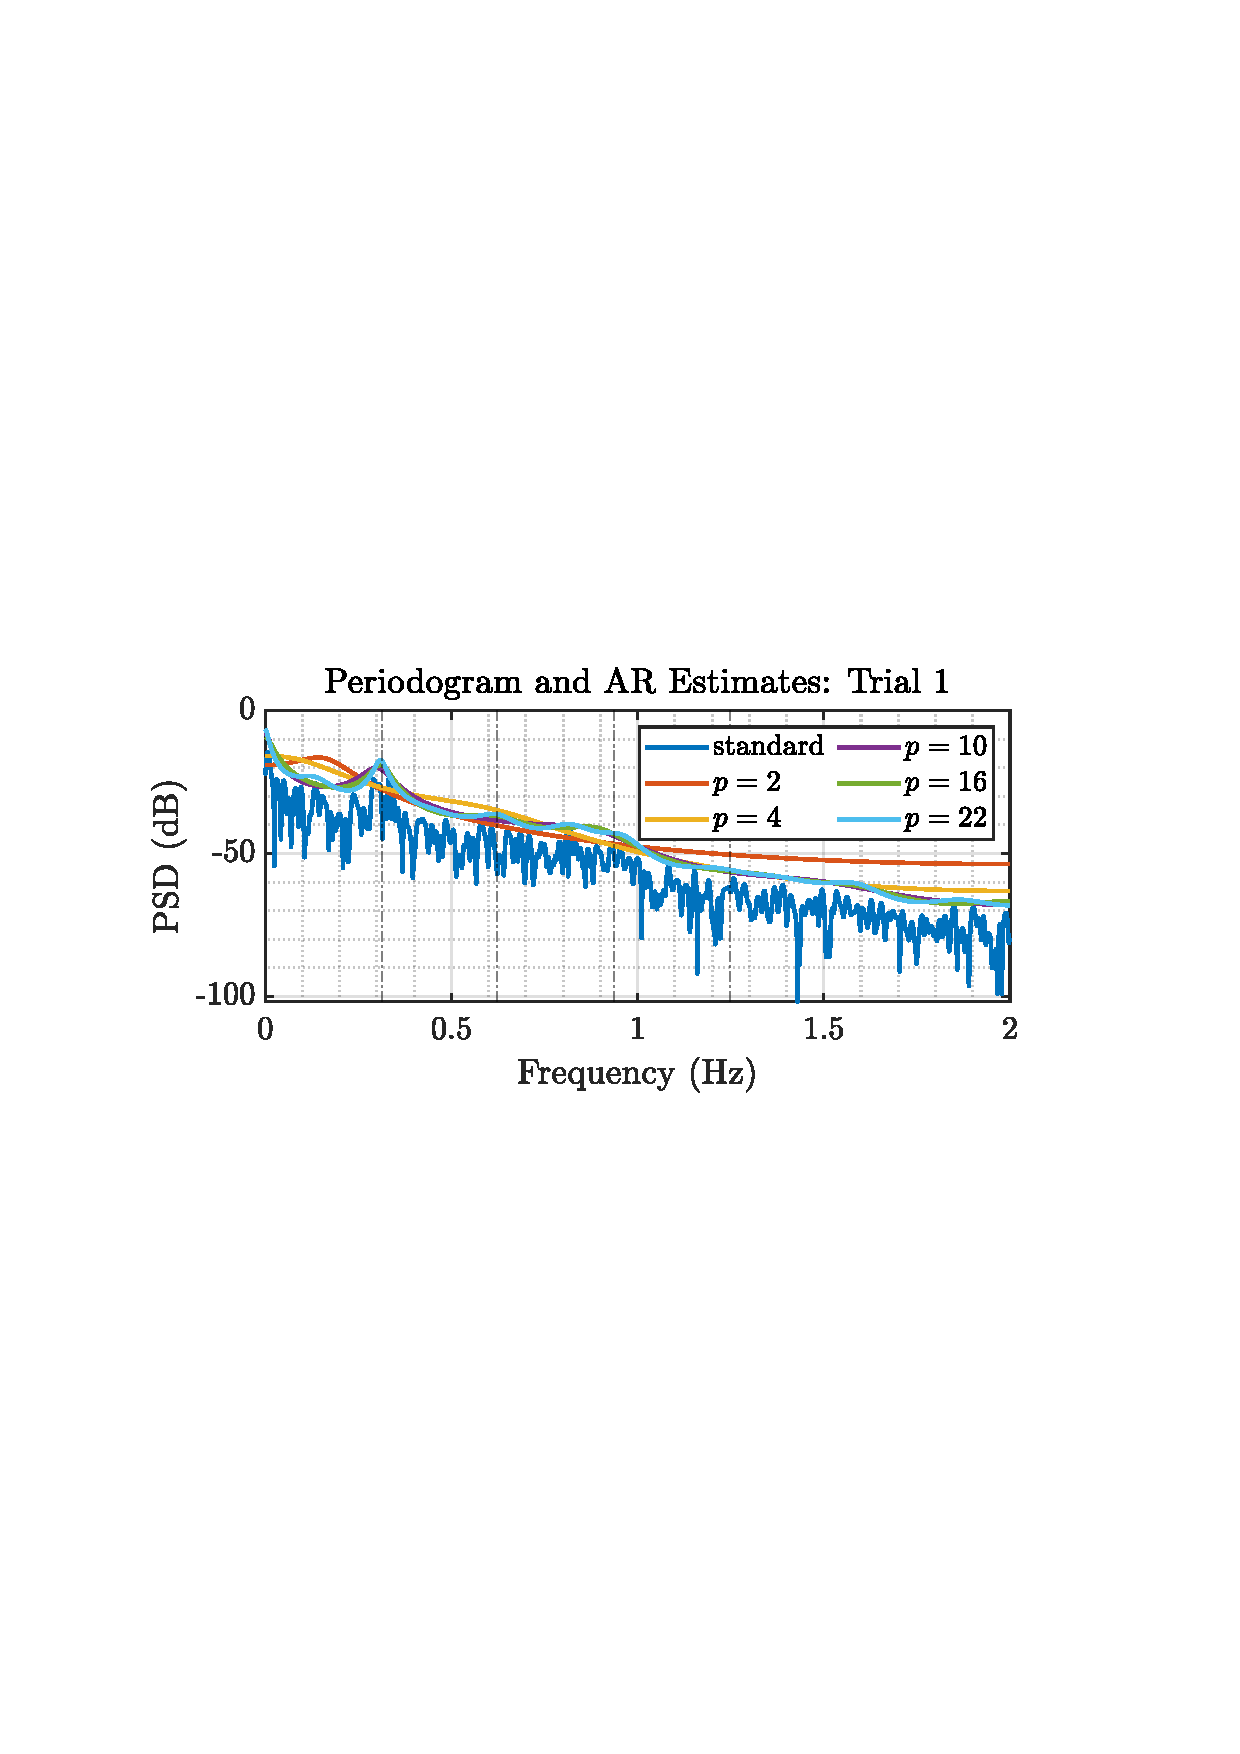
\includegraphics[trim={2.2cm 11.2cm 3.15cm  11.2cm}, clip, width=0.49\textwidth]{../MATLAB/figures/q1_5c_fig01.pdf} 
%		\end{centering}
%%		\vspace{-20pt}
%%		\vspace{-10pt}
%		\begin{centering}
%			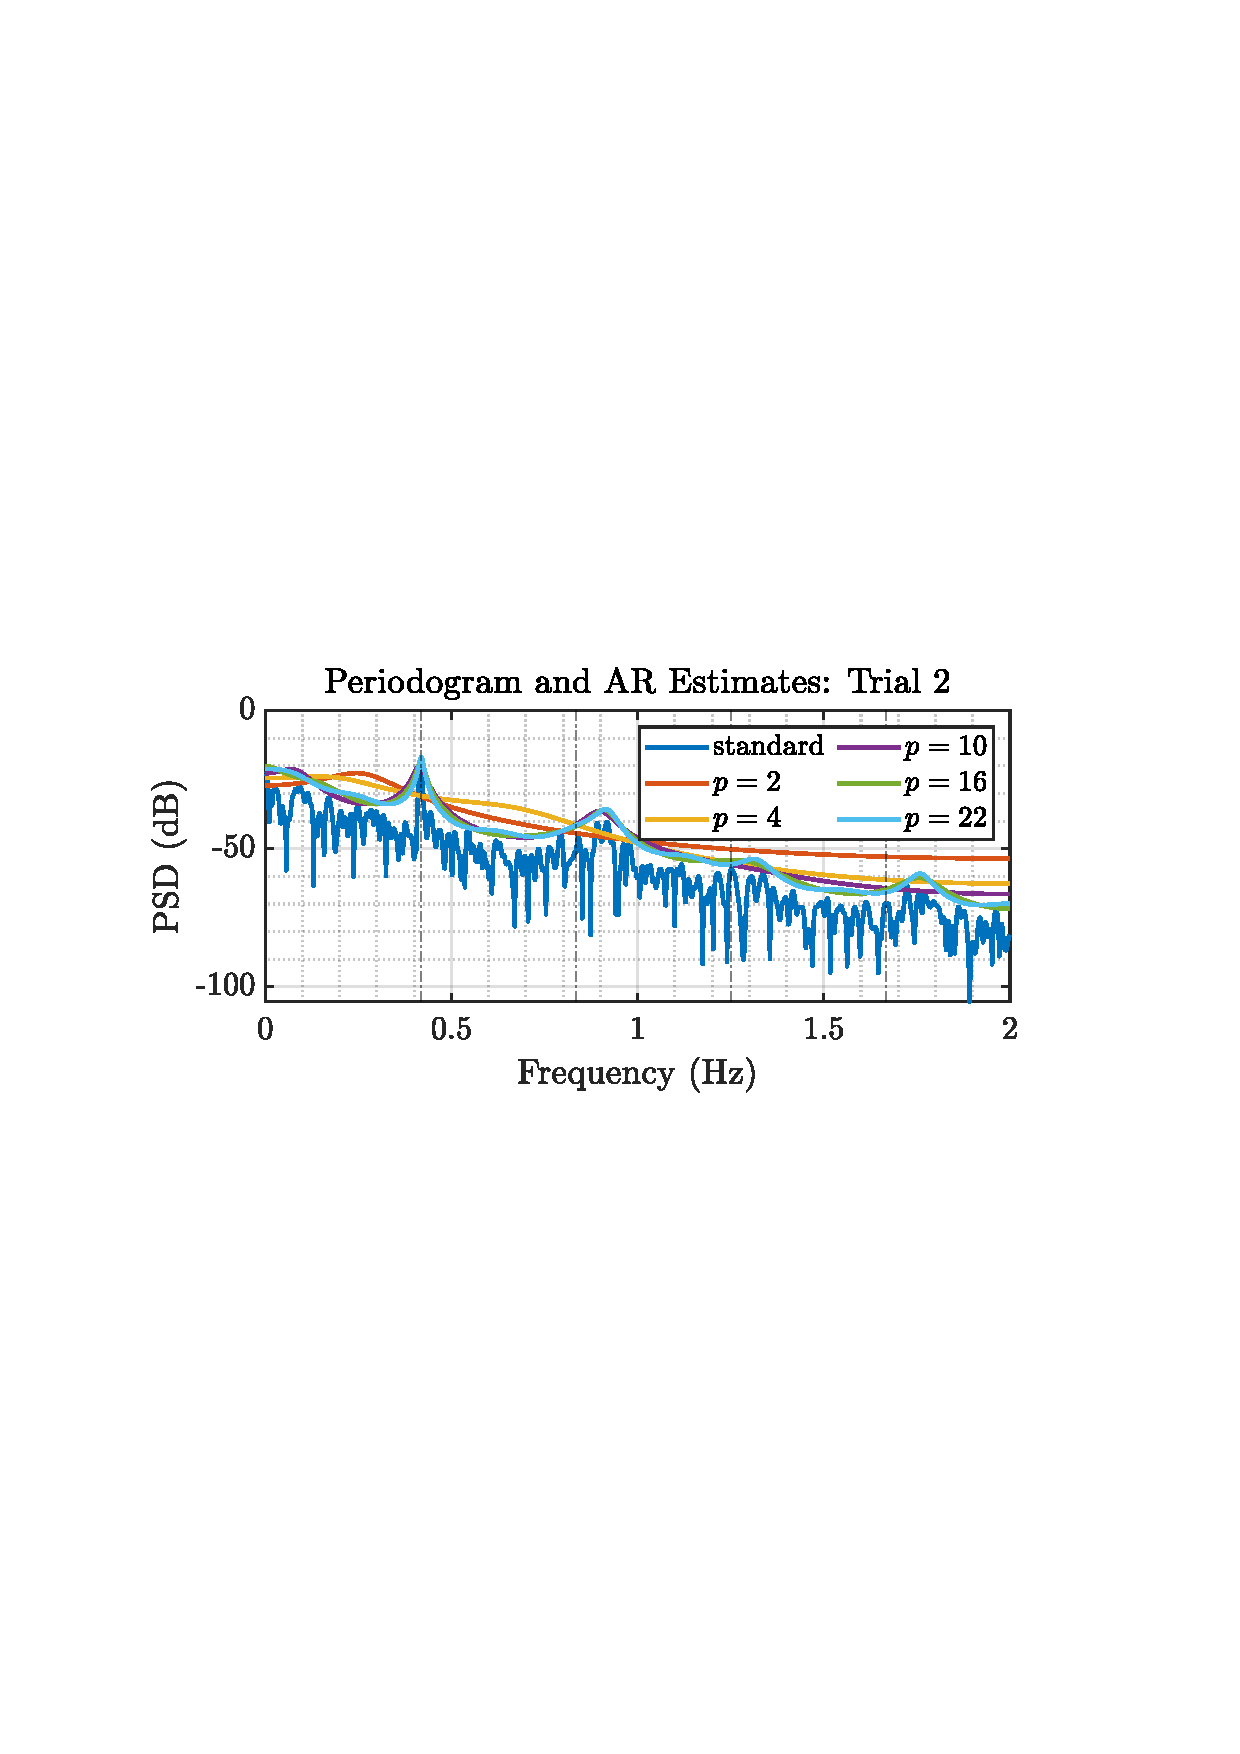
\includegraphics[trim={2.2cm 11.2cm 3.15cm  11.2cm}, clip, width=0.49\textwidth]{../MATLAB/figures/q1_5c_fig02.pdf} 
%		\end{centering}
%%		\vspace{-20pt}
%%		\vspace{-10pt}
%		\begin{centering}
%			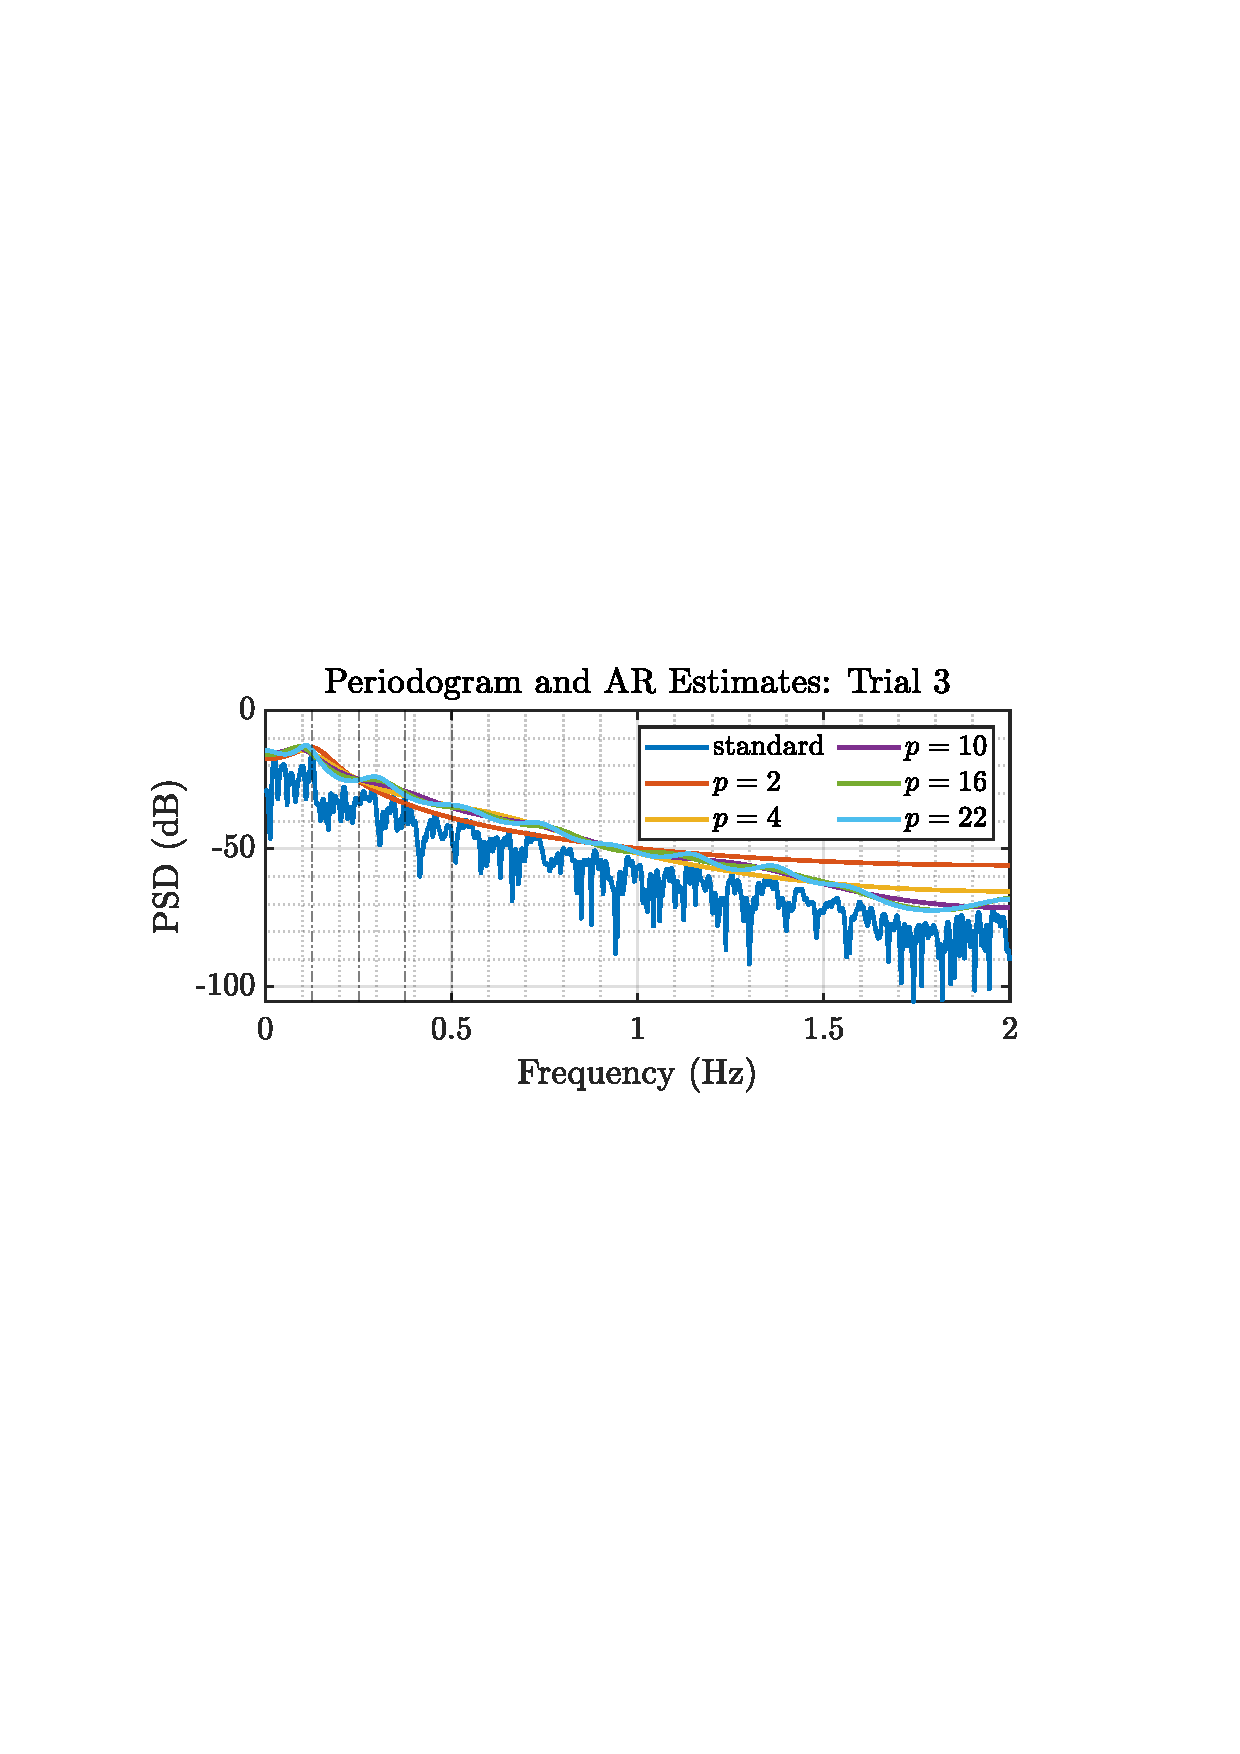
\includegraphics[trim={2.2cm 11.2cm 3.15cm  11.2cm}, clip, width=0.49\textwidth]{../MATLAB/figures/q1_5c_fig03.pdf} 
%		\end{centering}
%%		\vspace{-20pt}
%		\captionsetup{justification=centering}
%		\caption{AR Estimate Periodograms. \\ $p$ is the model order.}
%		\label{fig: 1-5c}
%%		\vspace{-10pt}
%	\end{wrapfigure}

		\begin{figure}[H]
			\begin{subfigure}{0.49\textwidth}
				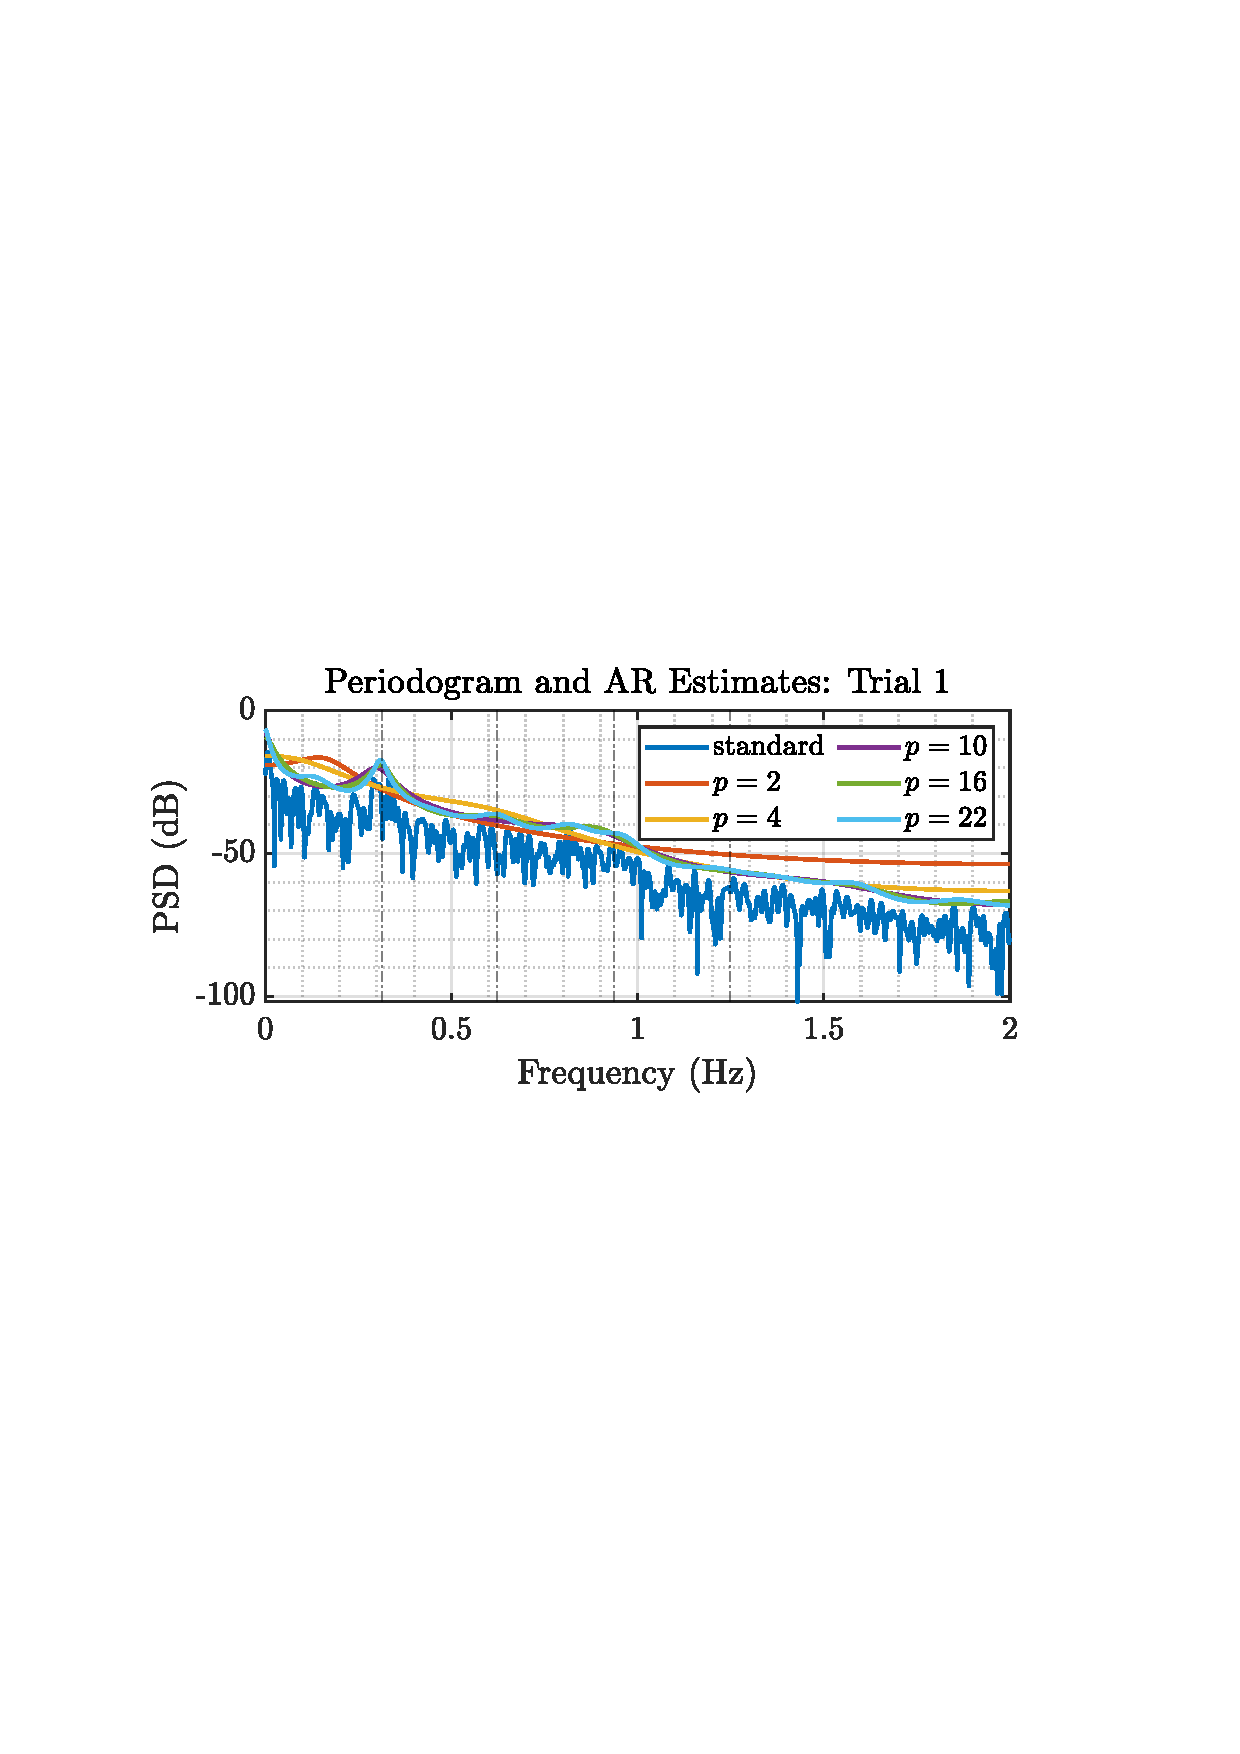
\includegraphics[trim={2.2cm 11.2cm 3.15cm  11.2cm}, clip, width=\textwidth]{../MATLAB/figures/q1_5c_fig01.pdf} 
				\caption{}
			\end{subfigure}
			\begin{subfigure}{0.49\textwidth}
				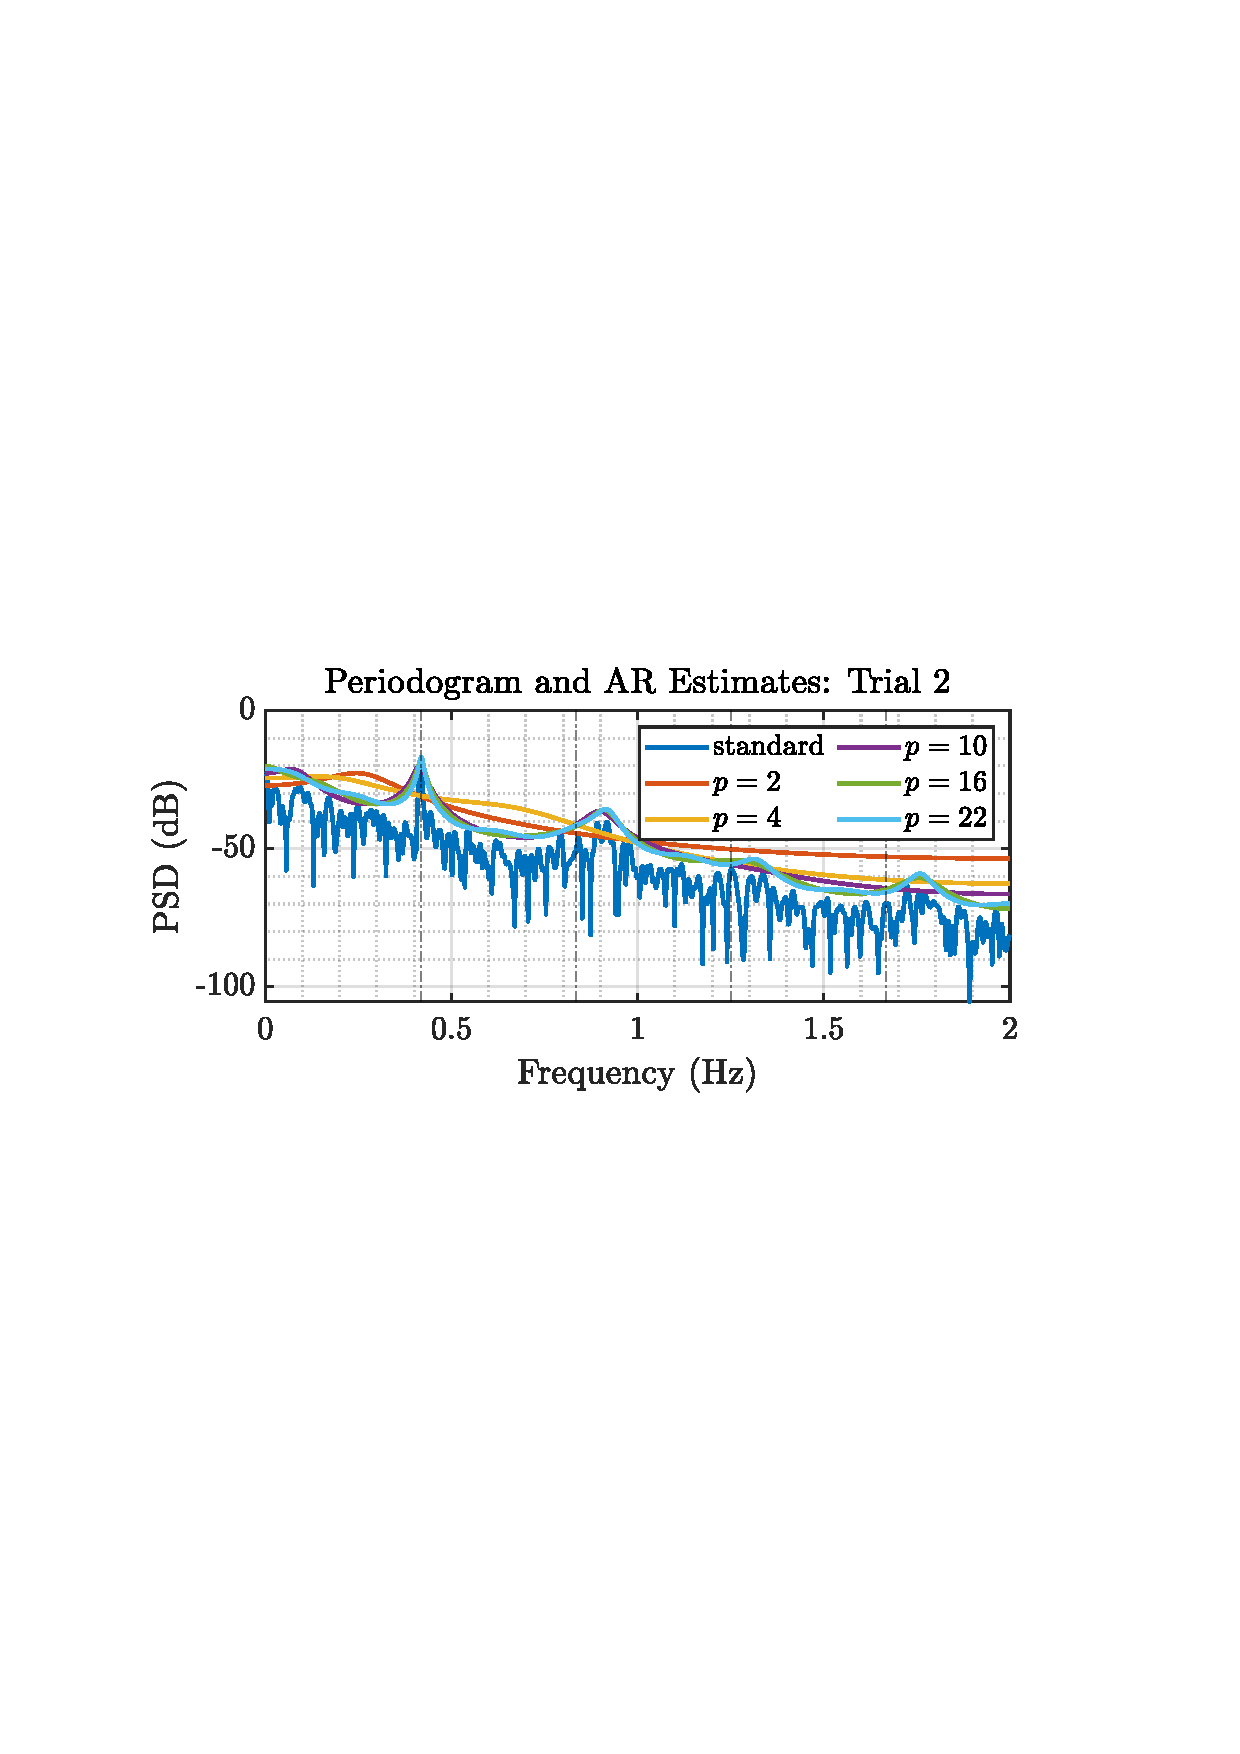
\includegraphics[trim={2.2cm 11.2cm 3.15cm  11.2cm}, clip, width=\textwidth]{../MATLAB/figures/q1_5c_fig02.pdf} 
				\caption{}
			\end{subfigure}%
%			\hspace*{0.25\textwidth}
%			\begin{subfigure}{0.49\textwidth}
%				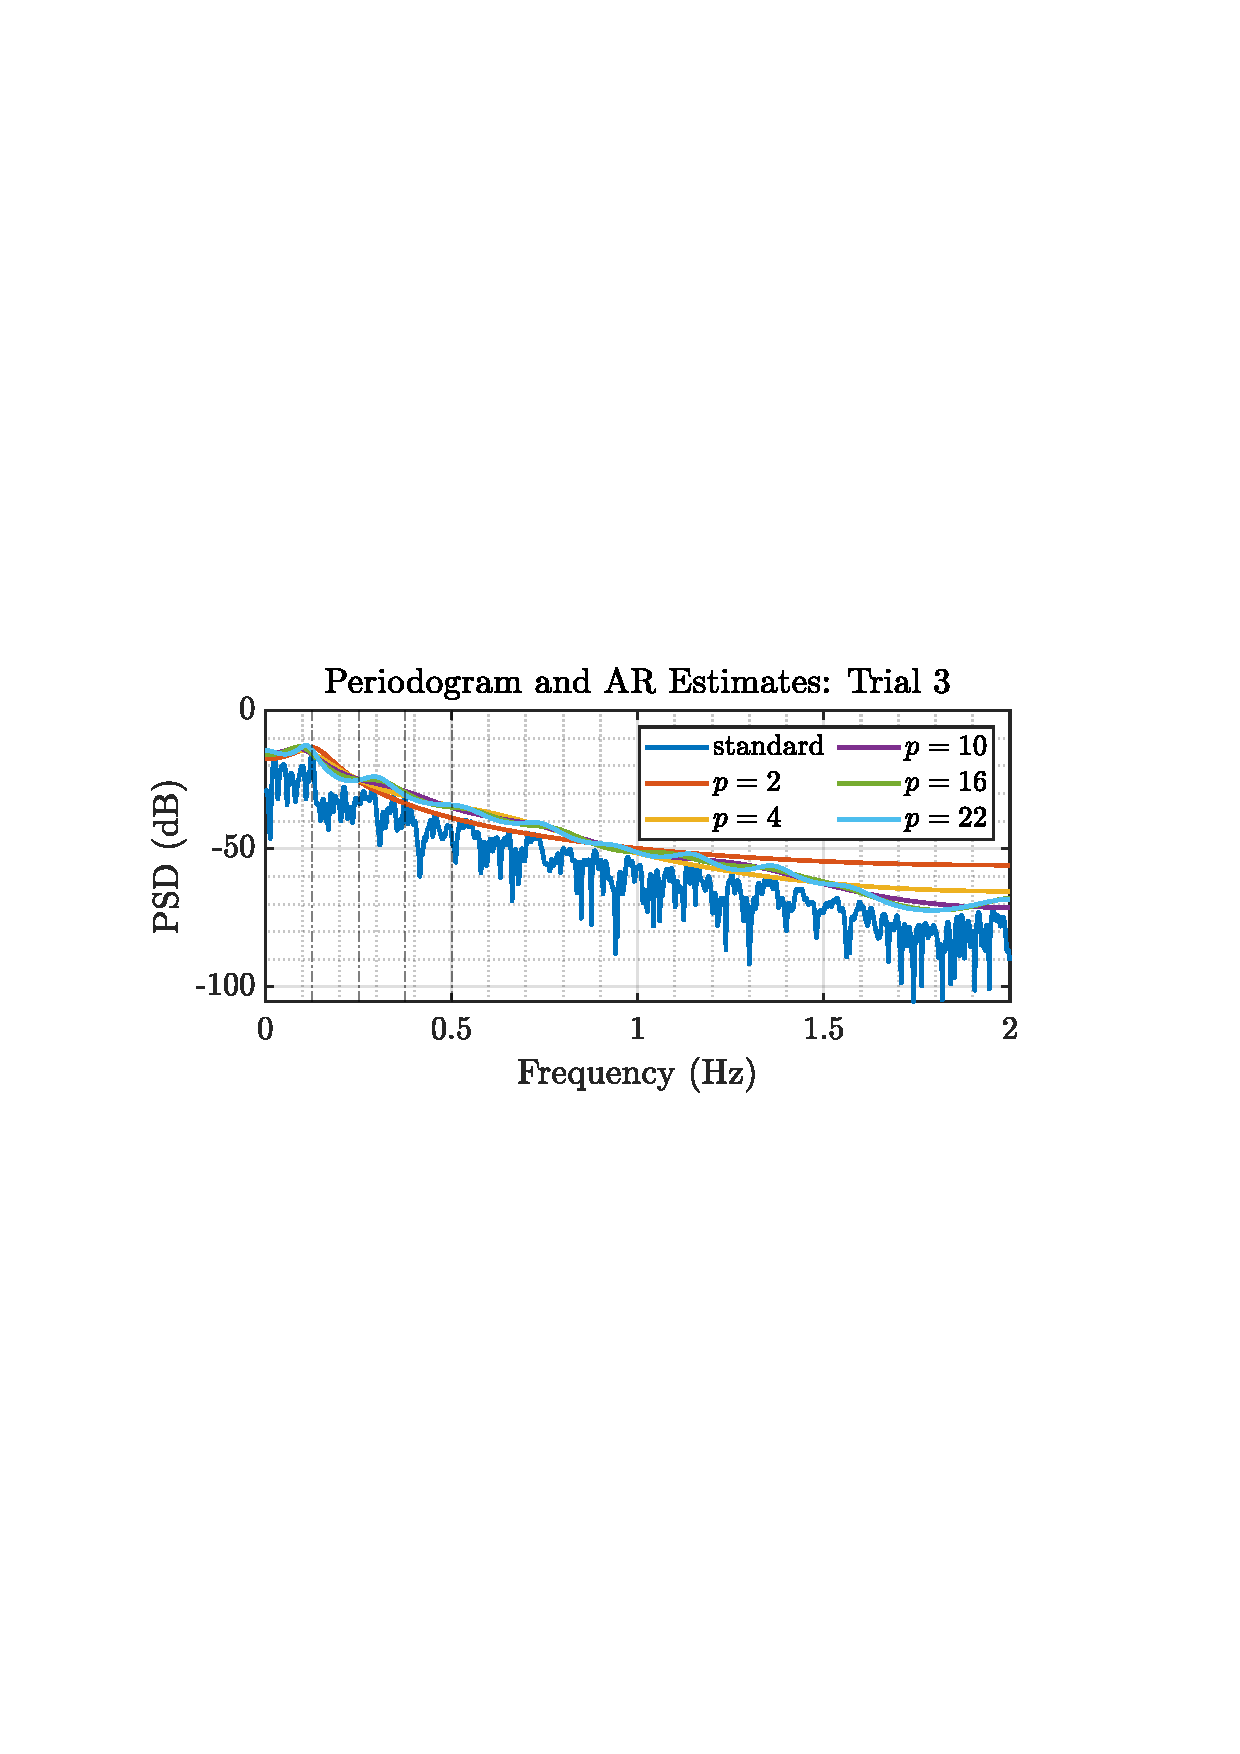
\includegraphics[trim={2.2cm 11.2cm 3.15cm  11.2cm}, clip, width=\textwidth]{../MATLAB/figures/q1_5c_fig03.pdf} 
%			\end{subfigure}
%			\captionsetup{justification=centering}
%			\caption{AR Estimate Periodograms. \\ $p$ is the model order.}
%			\label{fig: 1-5c}
			%		\vspace{-10pt}
			
			\begin{minipage}{0.46\textwidth}
				The AR spectral estimate in Figure \ref{fig: 1-5c} correctly identified the peak from models of order $p\gtrapprox10$. We note that the estimate resembles a smooth envelope over our PSD and correctly identifies clear peaks in the standard PSD at $p=10$. We also can see for higher order models that there are move fluctuations as the model starts to overfit for the input data's natural noisiness. \\
			\end{minipage}% 
			\begin{minipage}{0.04\textwidth}
				\hspace*{0.04\textwidth}
			\end{minipage}% 
			\begin{minipage}{0.49\textwidth}
				\begin{subfigure}{\textwidth}
					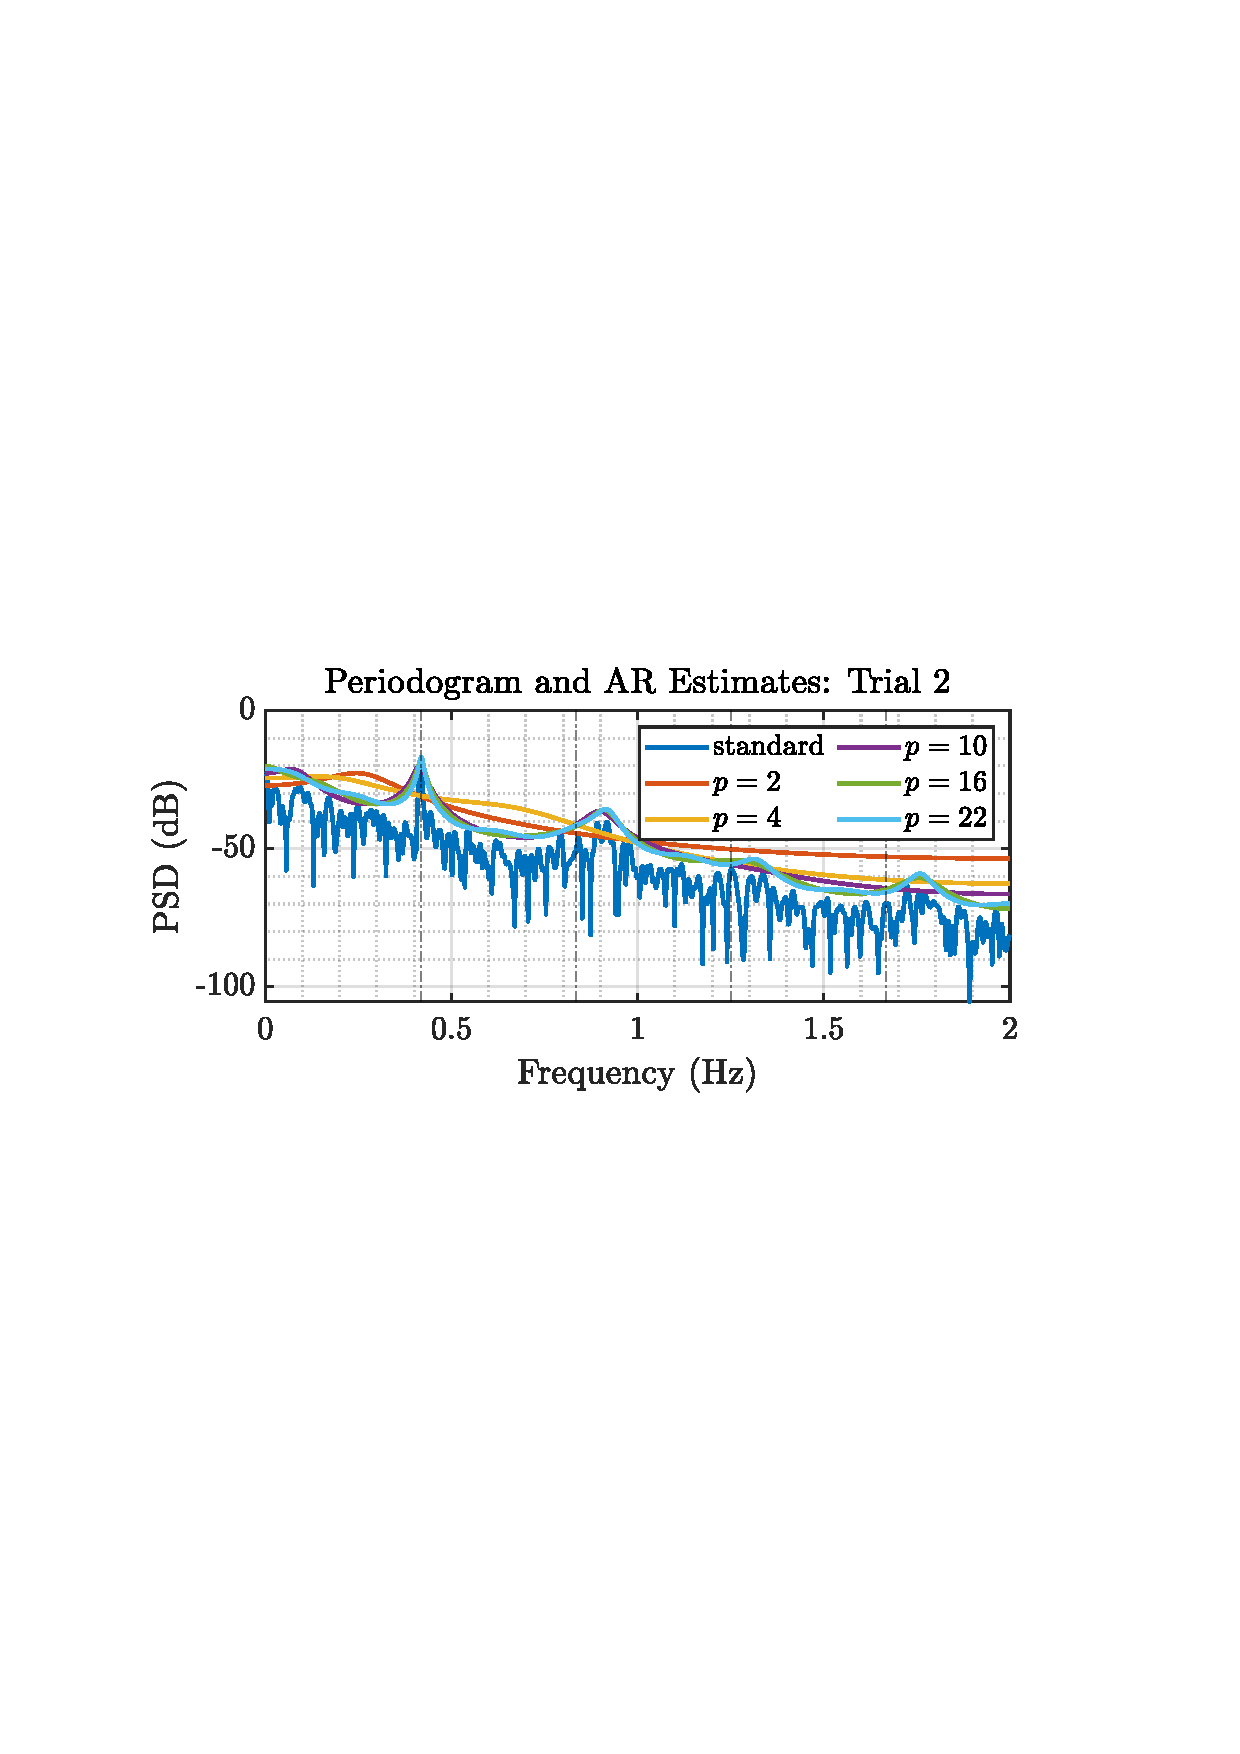
\includegraphics[trim={2.2cm 11.2cm 3.15cm  11.2cm}, clip, width=\textwidth]{../MATLAB/figures/q1_5c_fig02.pdf} 
					\caption{}
				\end{subfigure}%
%				\centering
%				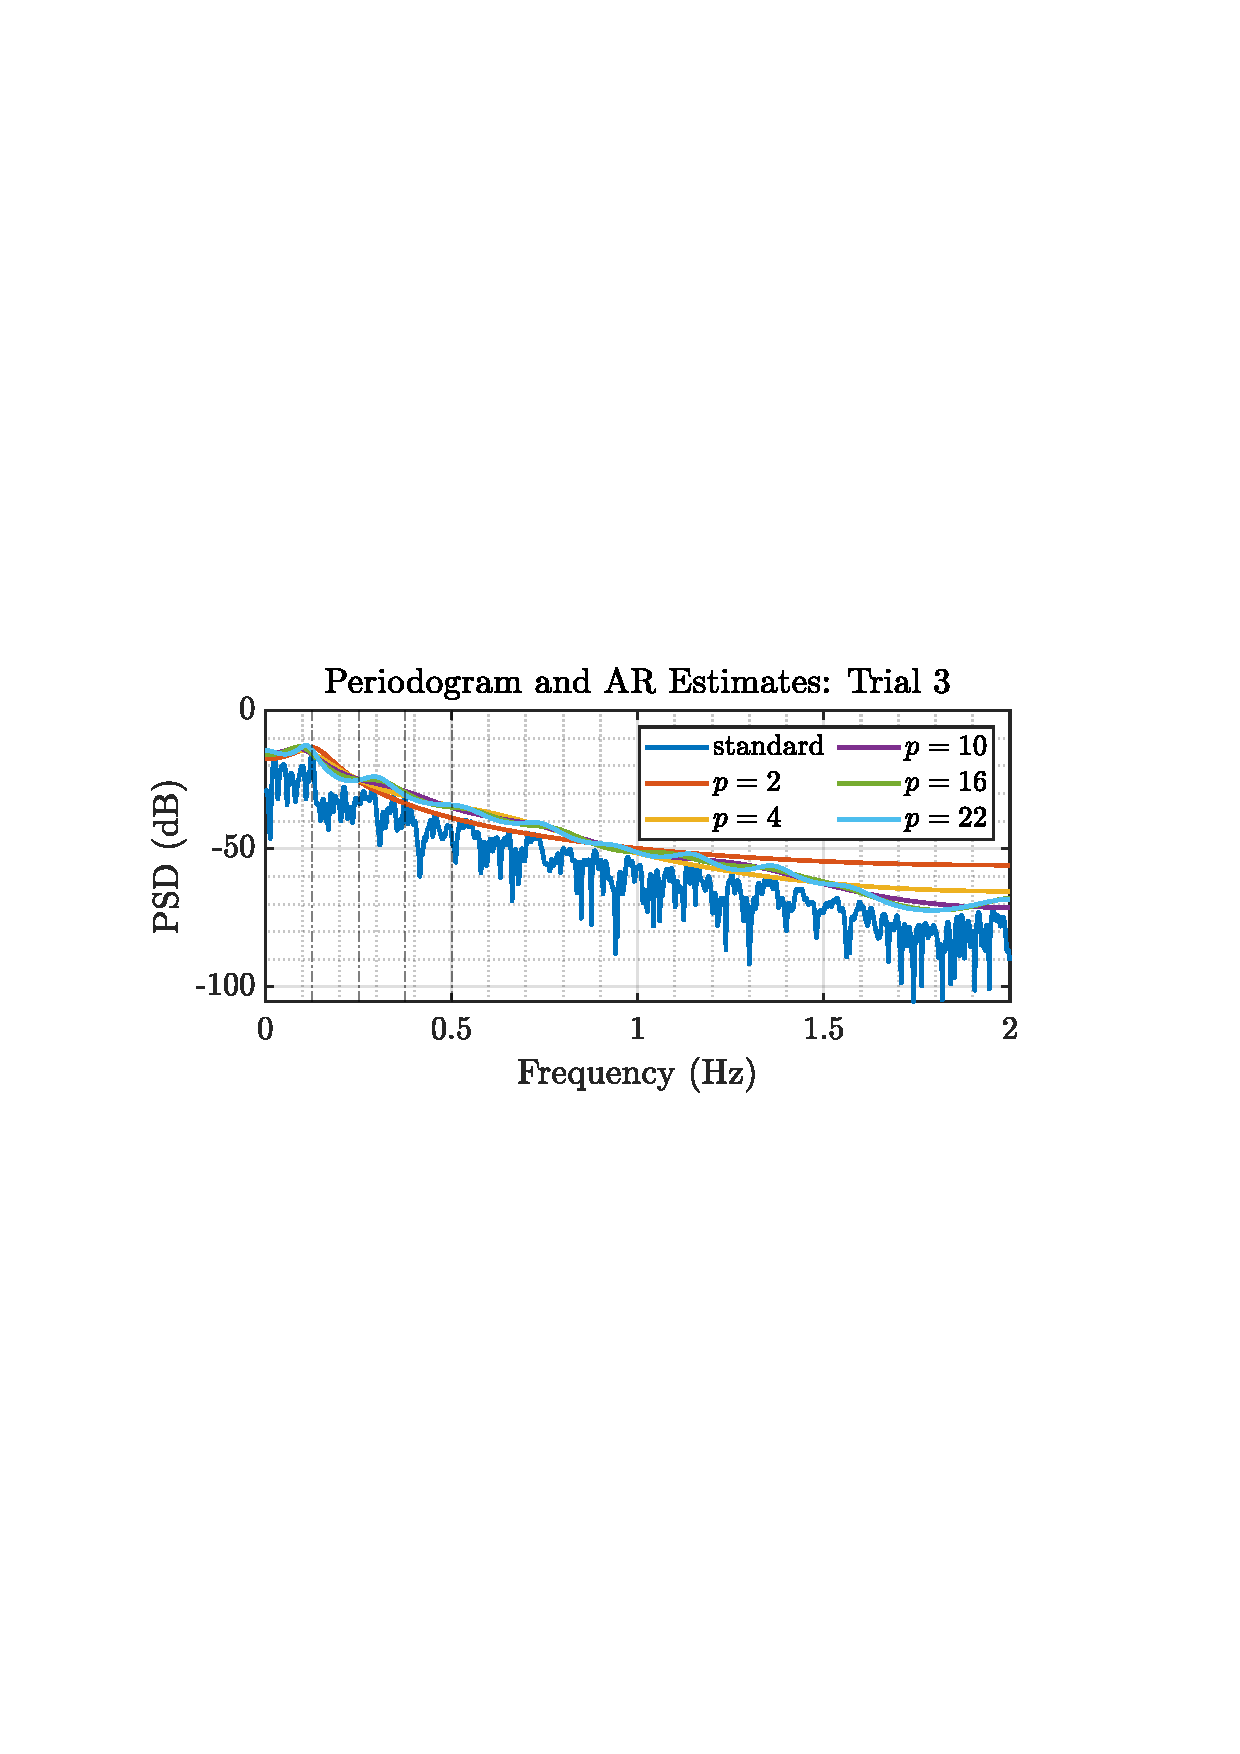
\includegraphics[trim={2.2cm 11.2cm 3.15cm  11.2cm}, clip, width=\textwidth]{../MATLAB/figures/q1_5c_fig03.pdf} 
				\captionsetup{justification=centering}
				\captionof{figure}{AR Estimate Periodograms. \\ $p$ is the model order.}
				\label{fig: 1-5c}
			\end{minipage}%
		\end{figure}
	

%	\pagebreak
	
	
	\subsection{Robust Regression} \label{sec: 1-6-robust-regression} 
	 	\subsubsection{Single Value Decomposition (SVD)}
			\begin{figure}[H]
				\centering
				\begin{subfigure}{0.49\textwidth}
					\centering
					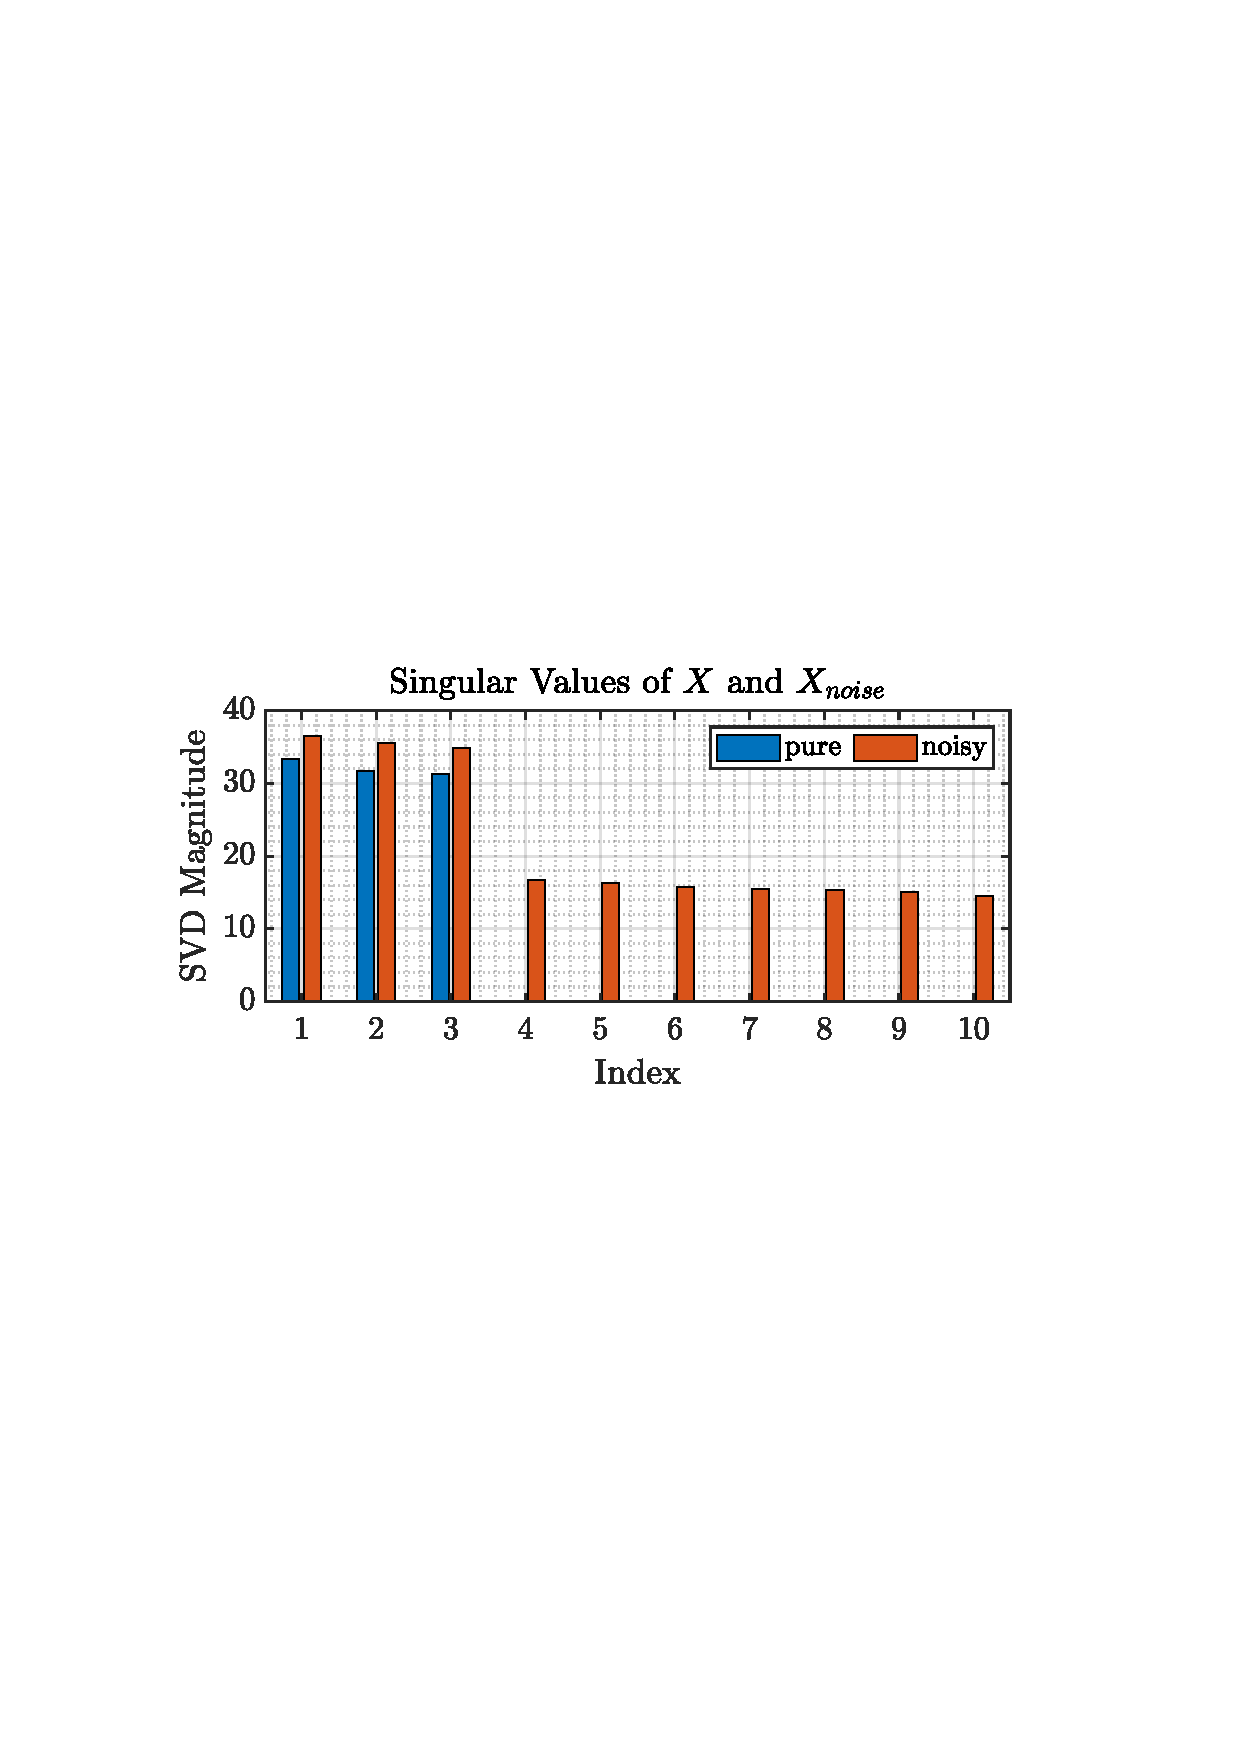
\includegraphics[trim={2.2cm 11.2cm 3.15cm  11.2cm}, clip, width=\textwidth]{../MATLAB/figures/q1_6a_fig01.pdf} 
					\captionsetup{justification=centering}
					\caption{SVD}
				\end{subfigure}
				%		~ % forces onto the same row
				\begin{subfigure}{0.49\textwidth}
					\centering
					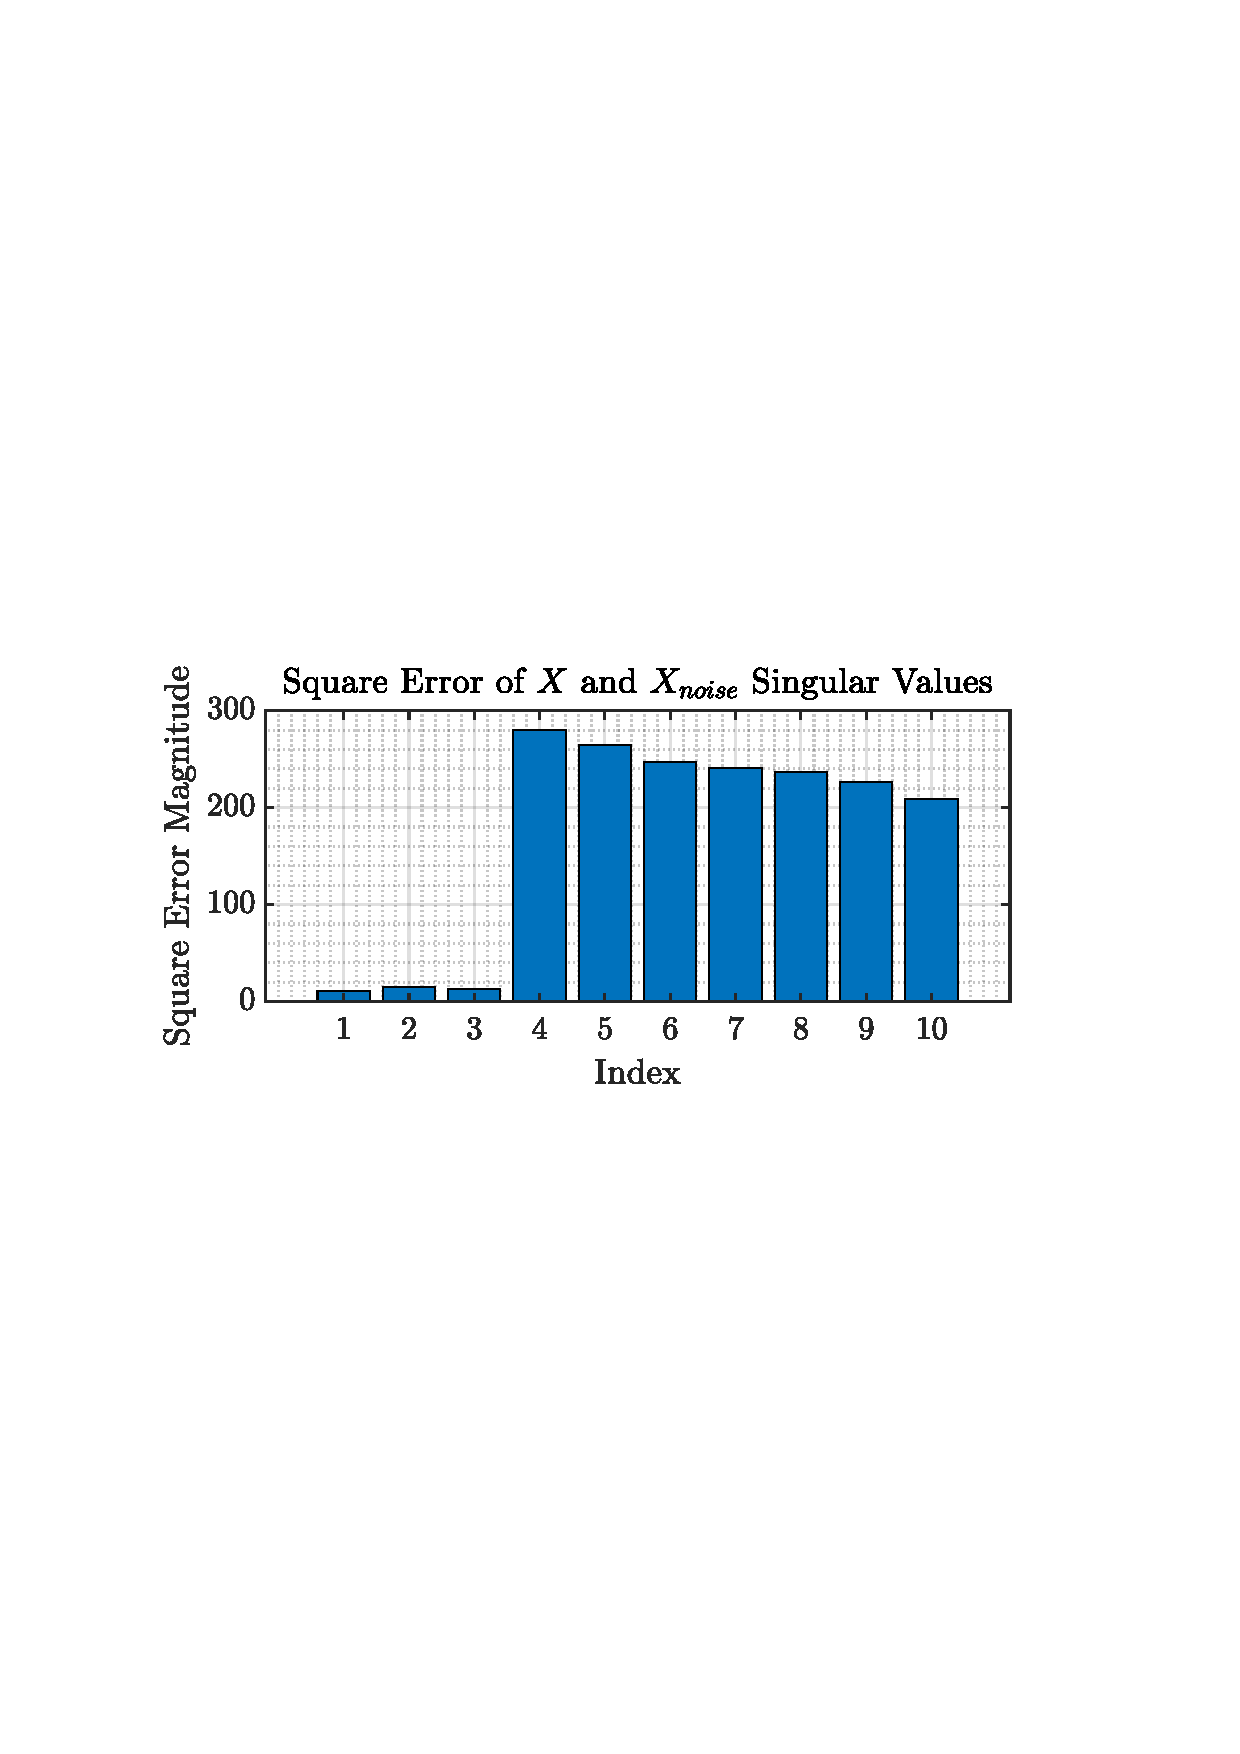
\includegraphics[trim={2.2cm 11.2cm 3.15cm  11.2cm}, clip, width=\textwidth]{../MATLAB/figures/q1_6a_fig02.pdf} 
					\captionsetup{justification=centering}
					\caption{Square Error}
				\end{subfigure}
				\captionsetup{justification=centering}
				\caption{}
				\label{fig: 1-6a}
			\end{figure}
		
		
		
			The rank of the input data would be indicated when the SVD Error increases or the non-zero SVD values end (for pure data) - hence the data is of rank 3. \\
			Noise makes the SVD magnitude non-zero where we expect it to be zero for the pure input. Hence, in the real world where we would not have the pure dataset we would need to purely look at Figure \ref{fig: 1-6a} (a), if the SVD magnitude of the noise was comparable to that of the signal we would have difficulty establishing a criteria to distinguish signal and noise subspaces from the SVD method. \\
	 
	% 	\pagebreak
	 	
	 	\subsubsection{Low Rank Approximation Error}
		 	\begin{minipage}[b]{0.49\textwidth}
			By looking at the mean square error between the pure signal and the low-rank approximation of the noise, Figure \ref{fig: 1-6b}, we note that the minimum error is when the low-rank approximation matches that of the pure data.
			\end{minipage}% 
			\begin{minipage}{0.04\textwidth}
				\hspace*{0.04\textwidth}
			\end{minipage}% 
			\begin{minipage}{0.49\textwidth}
				\centering
				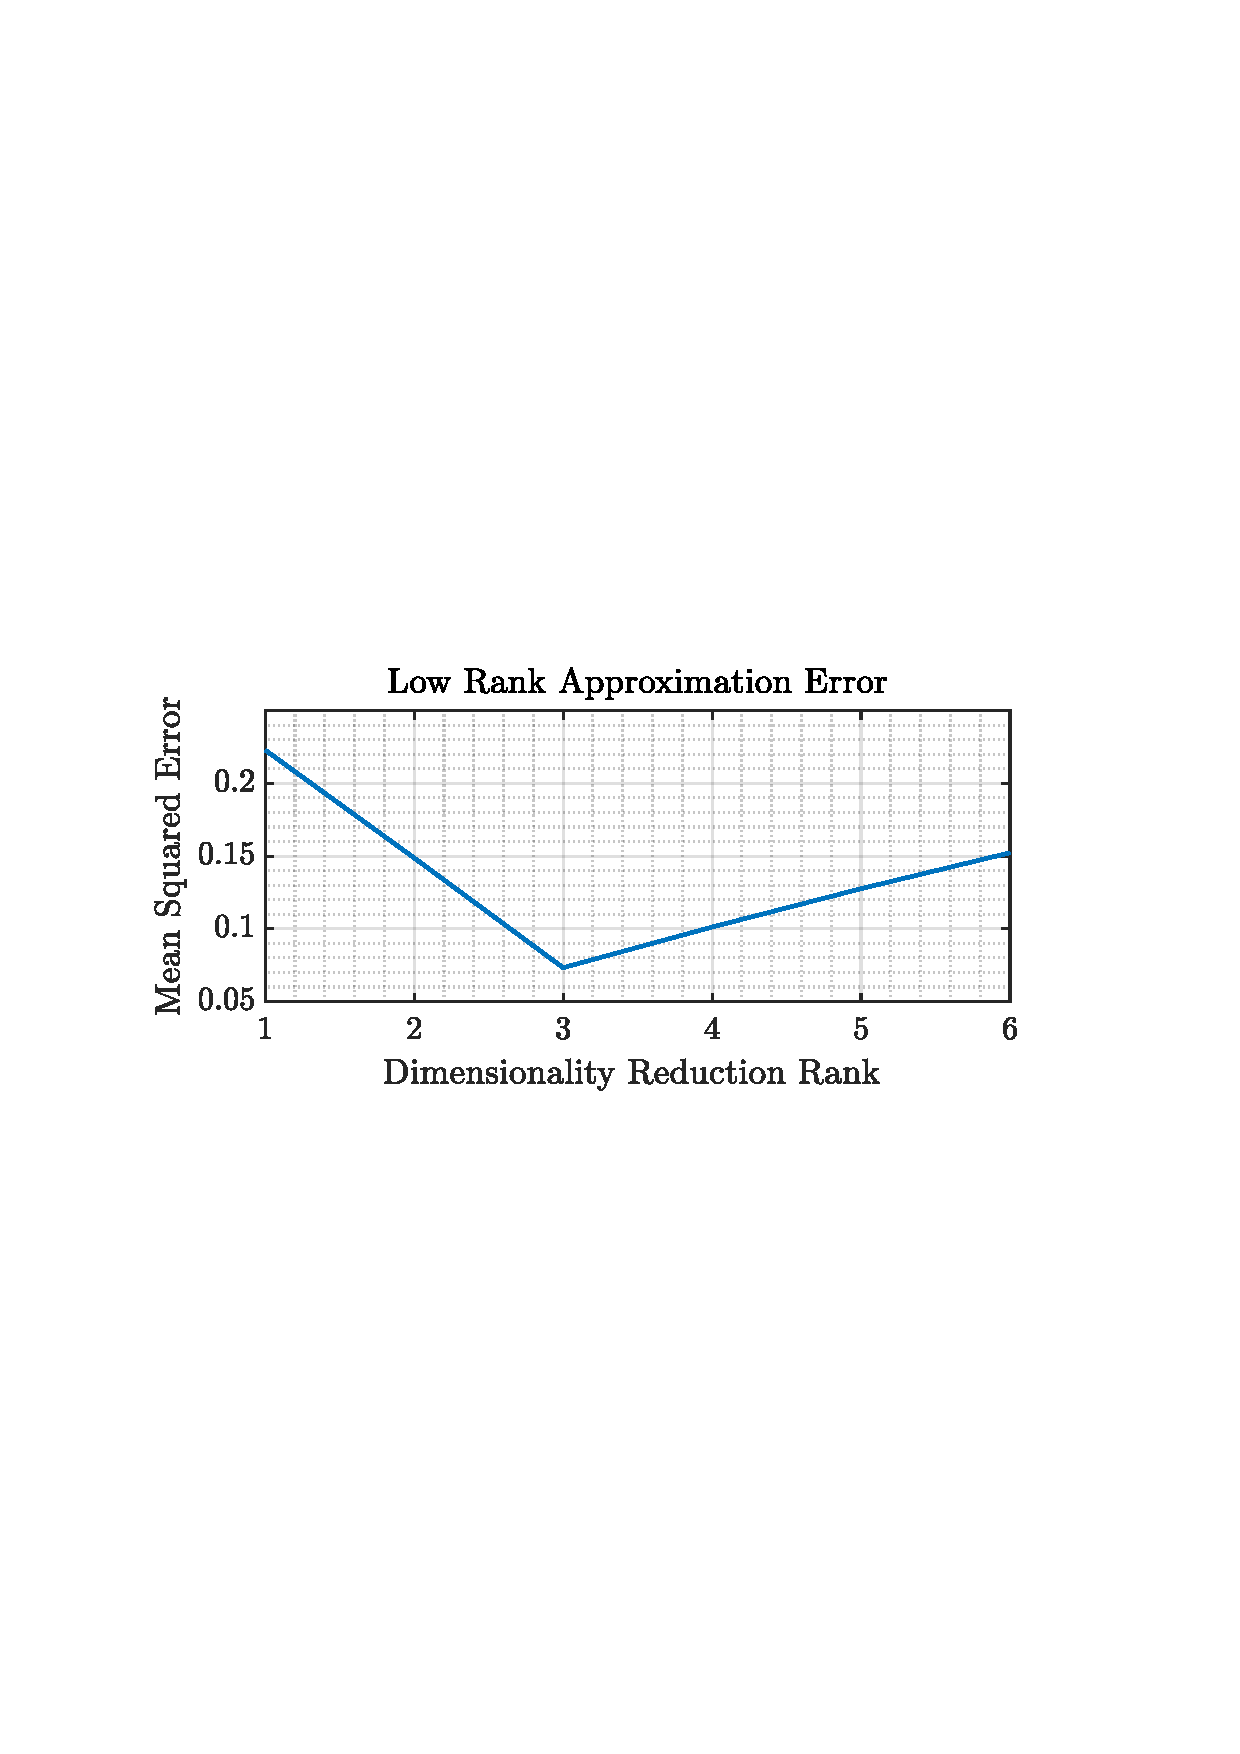
\includegraphics[trim={2.2cm 11.2cm 3.15cm  11.2cm}, clip, width=\textwidth]{../MATLAB/figures/q1_6b_fig01.pdf} 
				\captionsetup{justification=centering}
				\captionof{figure}{Effect of Changing Rank on the Approximation Error}
				\label{fig: 1-6b}
			\end{minipage}%
	
	 
	 	\subsubsection{Ordinary Least Squares (OLS) \& Principle Component Regression (PCR)  Estimate Errors}
	 	
		 	\begin{figure}[H]
		 		\centering
		 		\begin{subfigure}{0.49\textwidth}
		 			\centering
		 			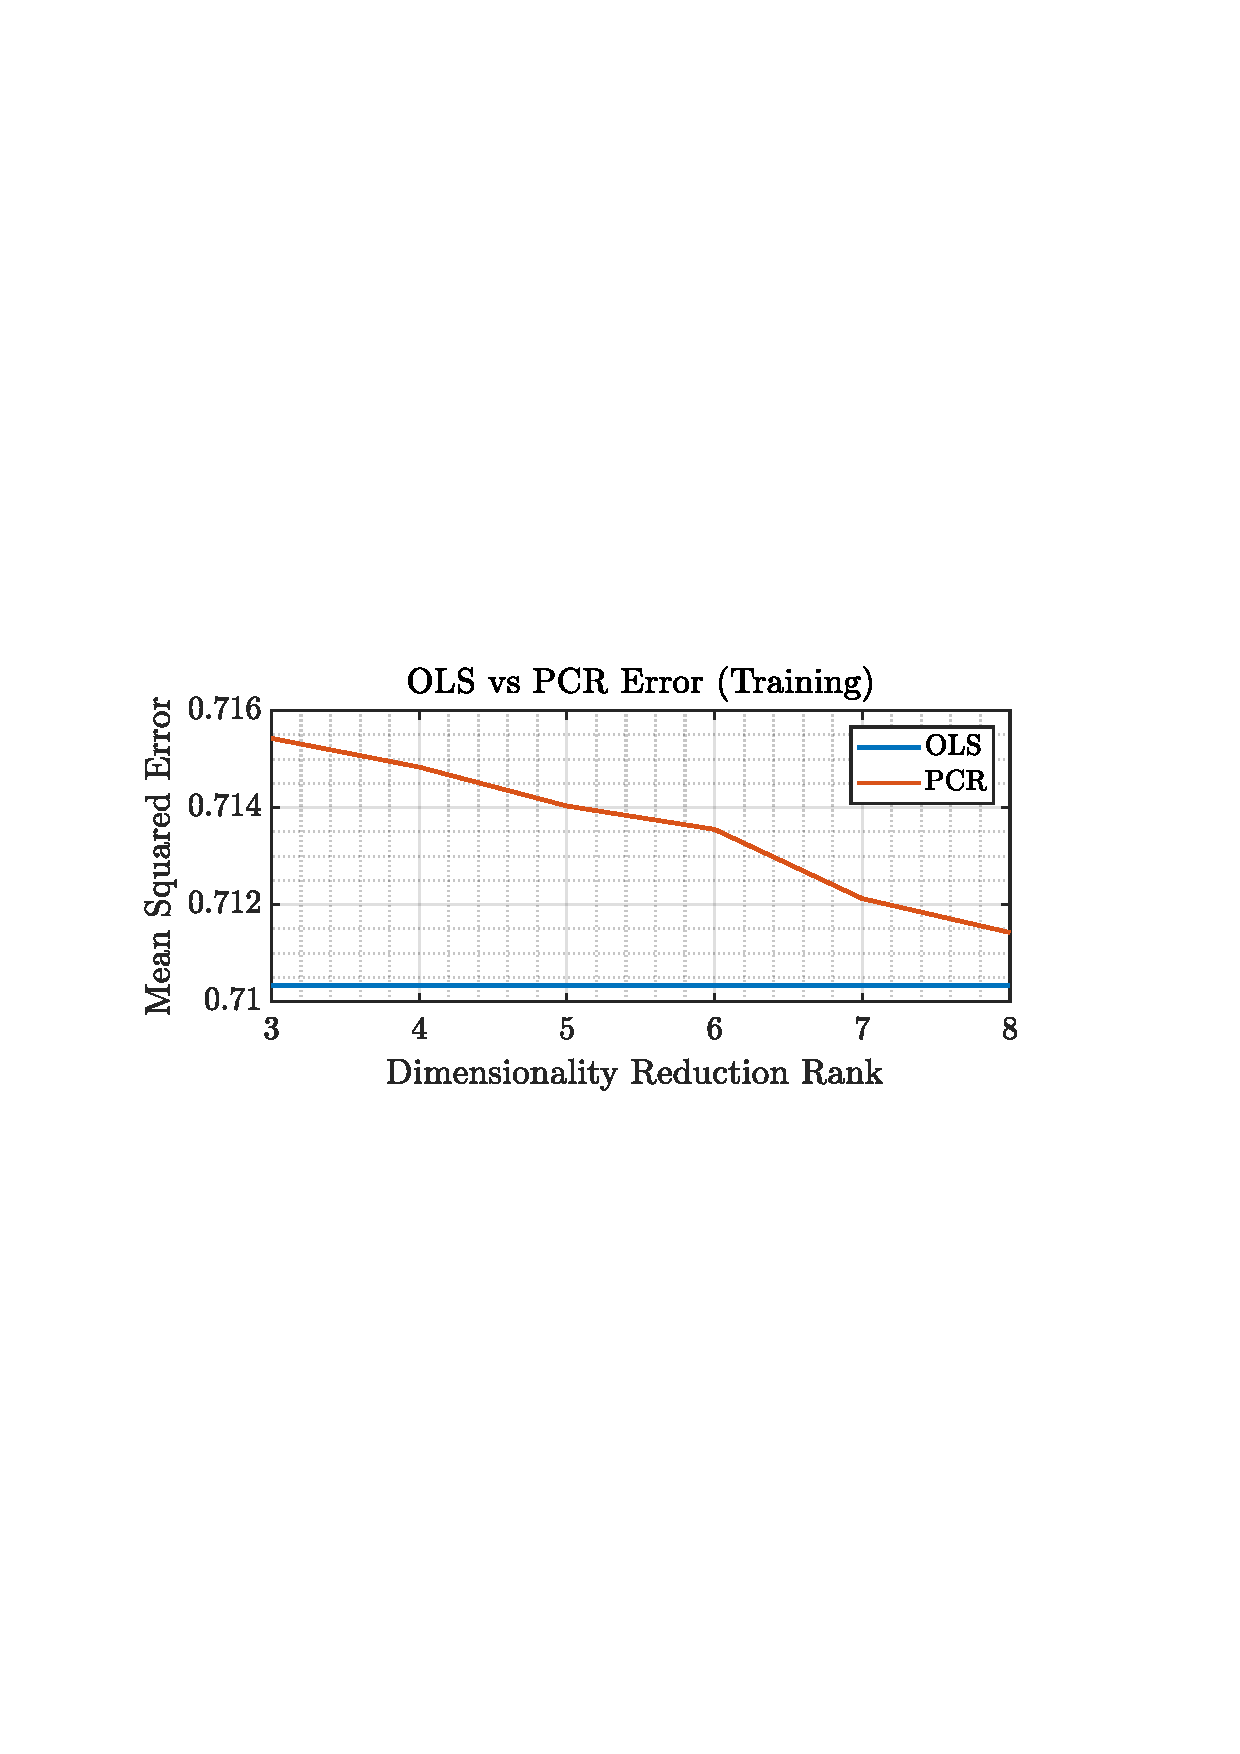
\includegraphics[trim={2.2cm 11.2cm 3.15cm  11.2cm}, clip, width=\textwidth]{../MATLAB/figures/q1_6c_fig01.pdf} 
		 			\captionsetup{justification=centering}
		 			\caption{Training Dataset Error}
		 		\end{subfigure}
		 		%		~ % forces onto the same row
		 		\begin{subfigure}{0.49\textwidth}
		 			\centering
		 			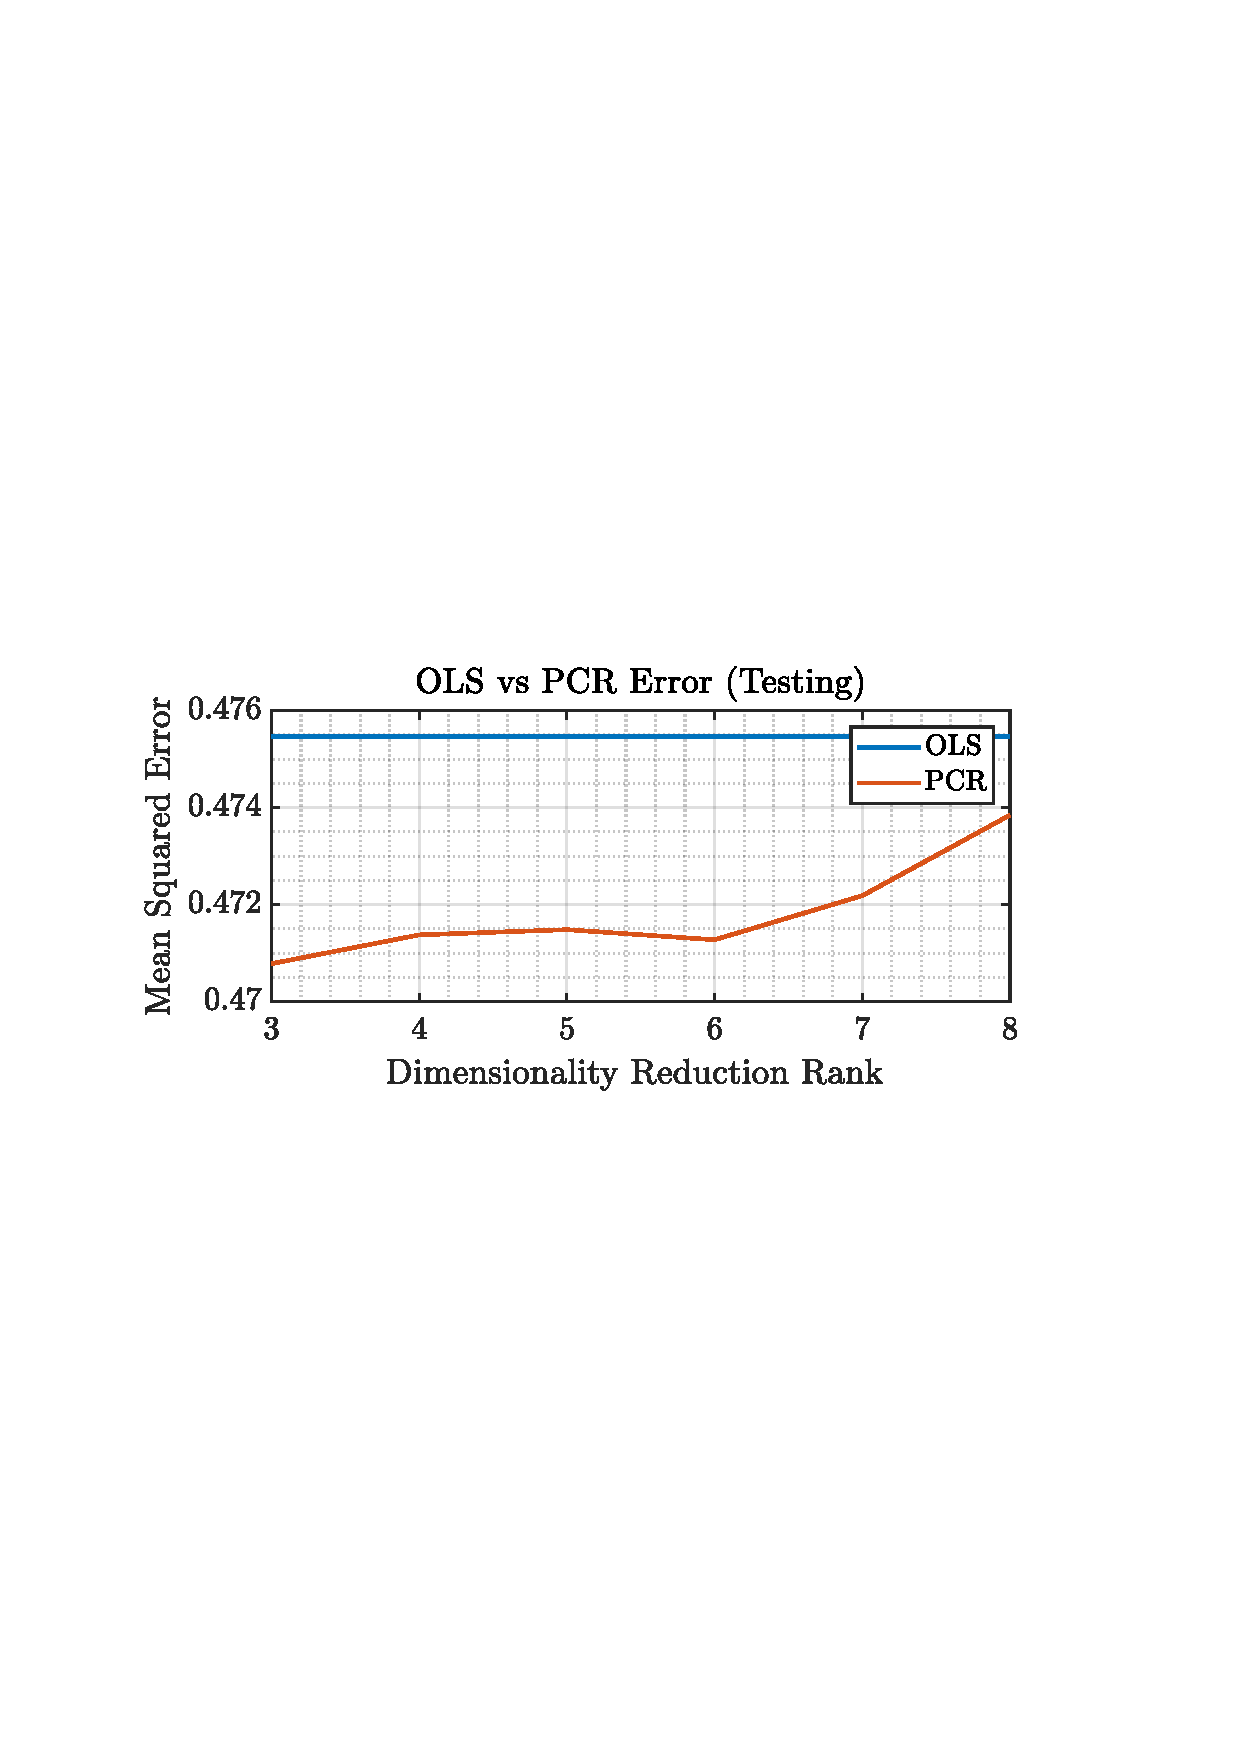
\includegraphics[trim={2.2cm 11.2cm 3.15cm  11.2cm}, clip, width=\textwidth]{../MATLAB/figures/q1_6c_fig02.pdf} 
		 			\captionsetup{justification=centering}
		 			\caption{Testing Dataset Error}
		 		\end{subfigure}
		 		\captionsetup{justification=centering}
		 		\caption{Comparison of Errors in the Training and Testing Datasets}
		 		\label{fig: 1-6c}
		 	\end{figure}
		 
		 	In both datasets we see that at the true model order the differences are tiny, in the training dataset we see that PCR underperforms by $0.85\%$, while in the testing dataset PCR outperforms by $1.05\%$. We can also note that decreasing the PCR model order further than the true model order, improves performance in the Training dataset but reduces performance in the Testing dataset.
		
		
	 	\subsubsection{Ordinary Least Squares (OLS) \& Principle Component Regression (PCR)  Estimate Errors - Part 2}
	 	\begin{minipage}{0.49\textwidth}
	 		Again if we look at the true model order, Figure \ref{fig: 1-6d}, PCR outperforms OLS by $0.79\%$. We note how further reduction in dimensionality decreases the performance of PCR. In regard to effectiveness of each scheme, if the model order is unknown and cannot be approximated accurately, OLS is a safer choice, however best performance - although marginal - can be achieved if the model order is known and PCR is implemented.
	 	\end{minipage}% 
		 \begin{minipage}{0.04\textwidth}
		 	  \hspace*{0.04\textwidth}
		 \end{minipage}% 
	 	\begin{minipage}{0.49\textwidth}
			\centering
	 		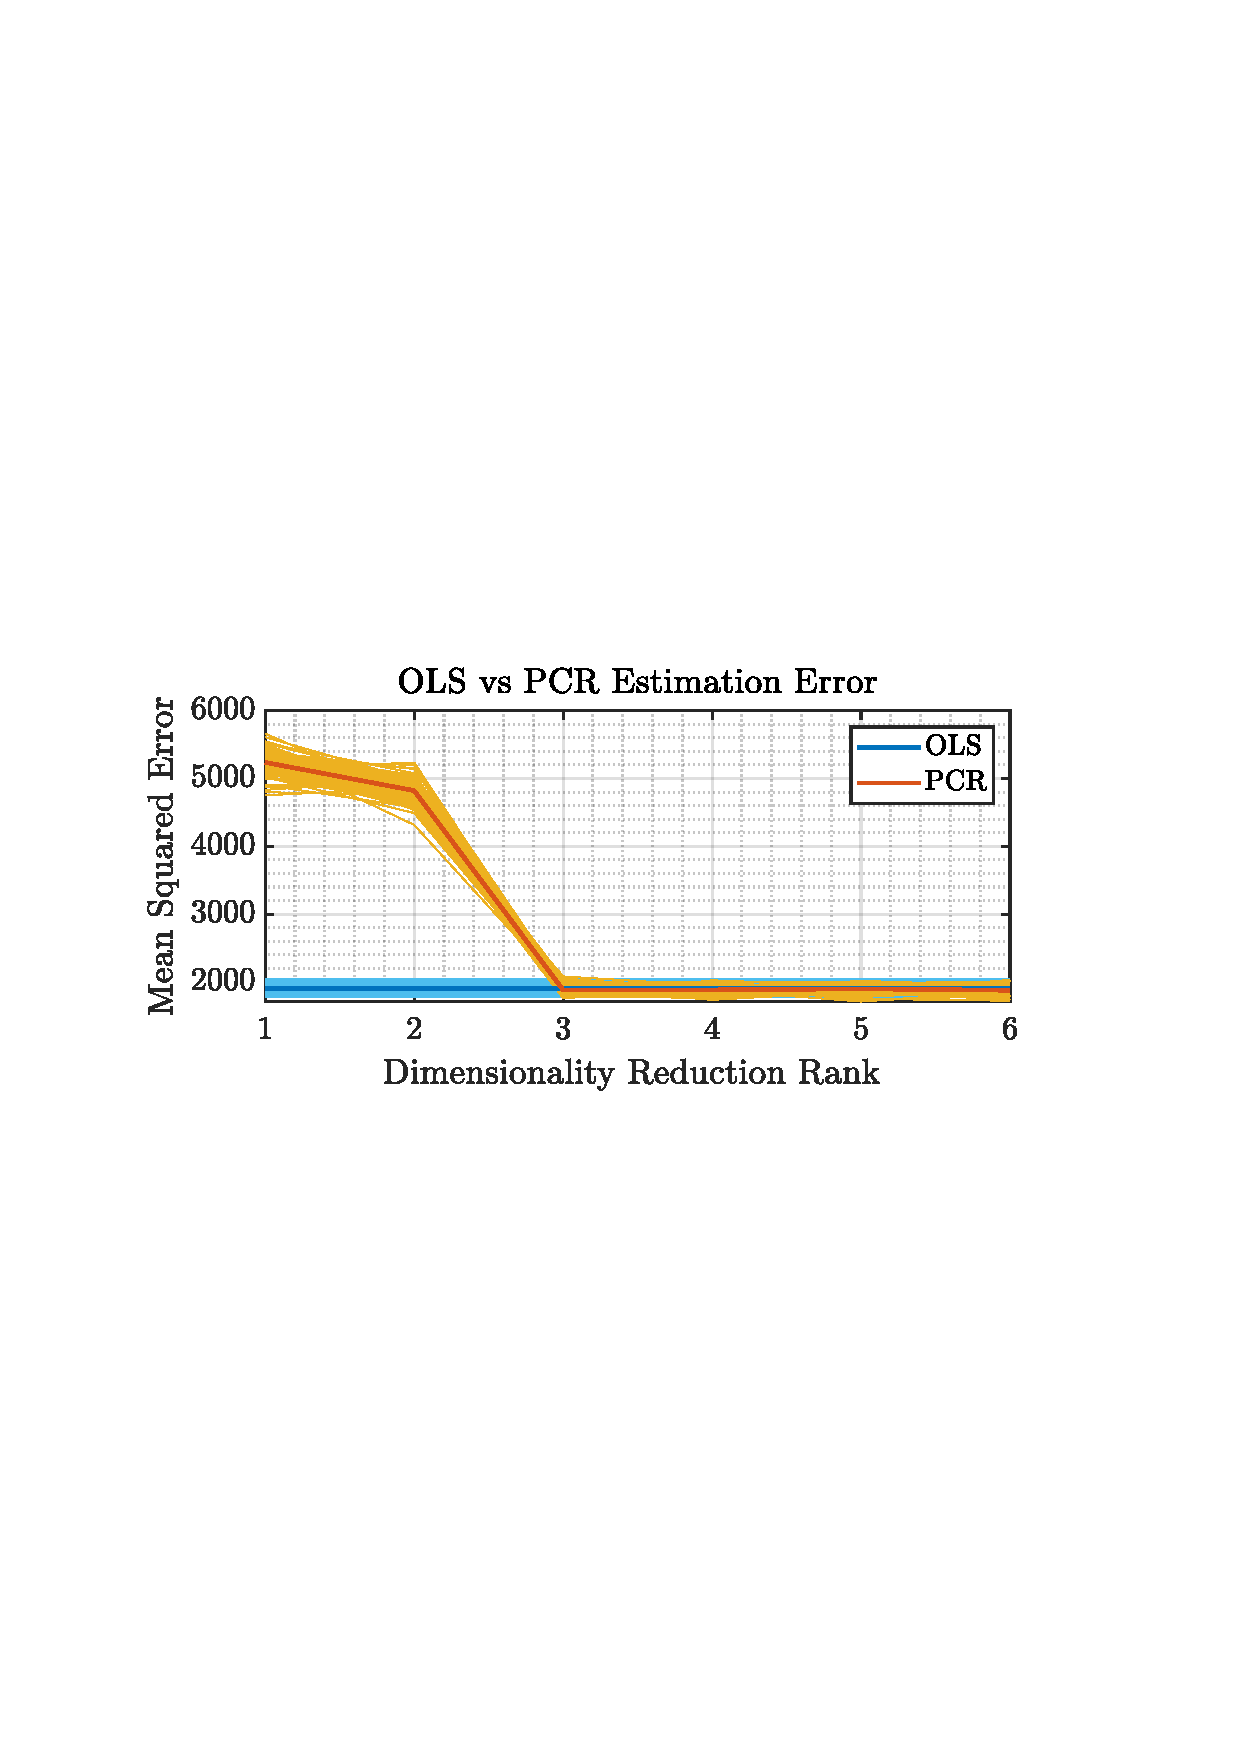
\includegraphics[trim={2.2cm 11.2cm 3.15cm  11.2cm}, clip, width=\textwidth]{../MATLAB/figures/q1_6d_fig01.pdf} 
	 		\captionsetup{justification=centering}
	 		\captionof{figure}{Mean Square Error over several Realisations}
	 		\label{fig: 1-6d}
	 	\end{minipage}%
 
\pagebreak
\section{Adaptive Signal Processing} \label{sec: 2-ASP}
	\subsection{The Least Mean Square (LMS) Algorithm} \label{sec: 2-1-LMS}
		\subsubsection{Example Correlation Matrix}
		\subsubsection{Example Learning Curve for an AR(2) Process}
			\begin{figure}[H]
				\centering
				\begin{subfigure}{0.49\textwidth}
					\centering
					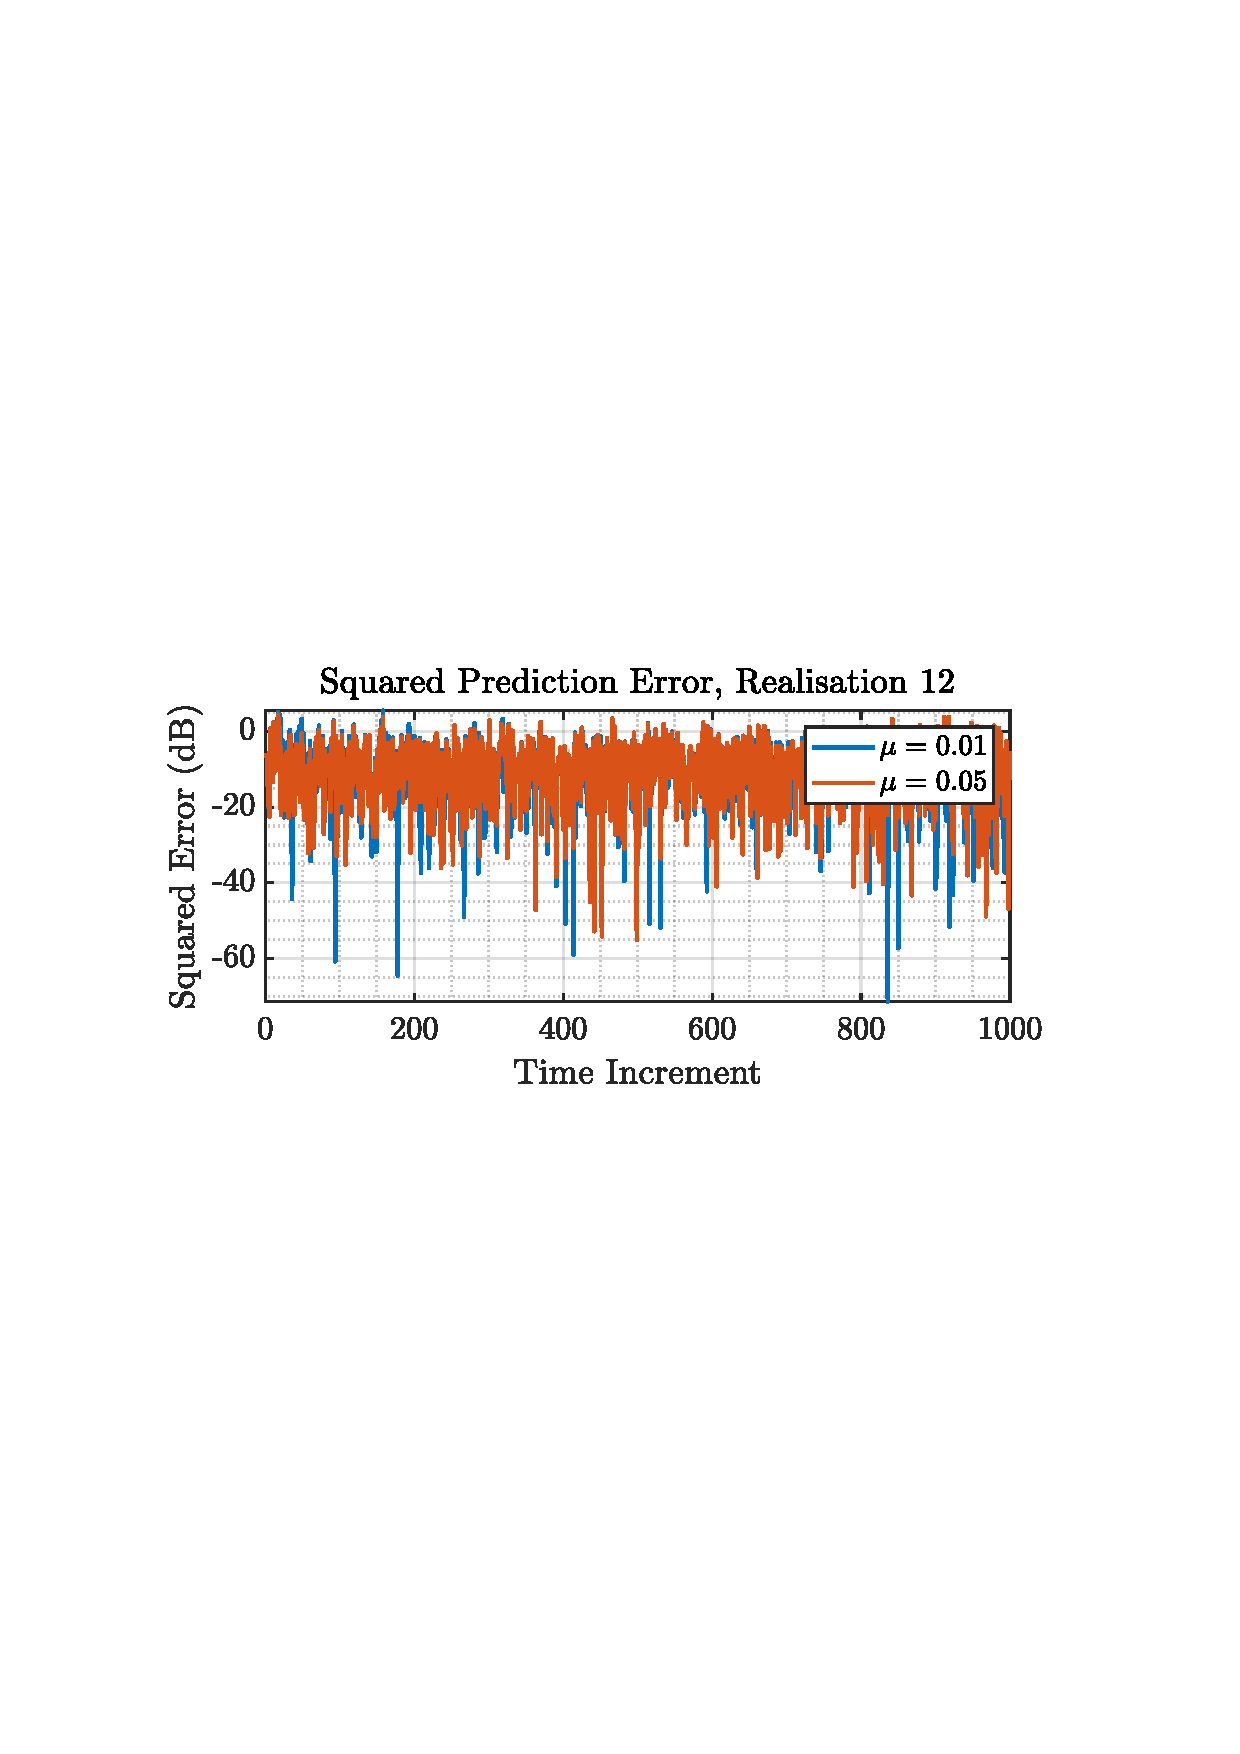
\includegraphics[trim={2.2cm 11.2cm 3.15cm  11.2cm}, clip, width=\textwidth]{../MATLAB/figures/q2_1b_fig01.pdf} 
					\captionsetup{justification=centering}
					\caption{Square Prediction Error, Single Realisation}
				\end{subfigure}
				%		~ % forces onto the same row
				\begin{subfigure}{0.49\textwidth}
					\centering
					\includegraphics[trim={2.2cm 11.2cm 3.15cm  11.2cm}, clip, width=\textwidth]{../MATLAB/figures/q2_1b_fig03.pdf} 
					\captionsetup{justification=centering}
					\caption{Log of Mean of the Squared Prediction Error}
				\end{subfigure}
				\captionsetup{justification=centering}
				\caption{$\mu$'s effect on the Squared Prediction Error and the Influence of the Log operator}
				\label{fig: 2-1b}
			\end{figure}
		\subsubsection{Misadjustment}
			\begin{minipage}[b]{0.49\textwidth}
				\begin{table}[H]
					\centering
					\begin{tabular}{|c|c||c|}
						\hline
						\textbf{$\mu$} & \textbf{$\mathcal{M}_{LMS}$} & \textbf{$\mathcal{M}_{theoretical}$} \\
						\hline
						\hline
						0.01 & $15$ & $0$ \\
						\hline
						0.005 & $2$ & $0$ \\
						\hline
					\end{tabular}
					\captionsetup{justification=centering}
					\caption{Theoretical and Estimated Misadjustments}
					\label{tab: 2-1c}
				\end{table}
			\end{minipage}% 
			\begin{minipage}{0.04\textwidth}
				\hspace*{0.04\textwidth}
			\end{minipage}% 
			\begin{minipage}{0.49\textwidth}
				\centering
				\includegraphics[trim={2.2cm 11.2cm 3.15cm  11.2cm}, clip, width=\textwidth]{../MATLAB/figures/q2_1f_fig01.pdf} 
				\captionsetup{justification=centering}
				\captionof{figure}{Estimated Misadjustment, varying with realisation}
				\label{fig: 2-1c}
			\end{minipage}%

		\subsubsection{Steady State Estimation} 
			\begin{figure}[H]
				\centering
				\begin{subfigure}{0.49\textwidth}
					\centering
					\includegraphics[trim={2.2cm 11.2cm 3.00cm  11.2cm}, clip, width=\textwidth]{../MATLAB/figures/q2_1cd_fig02.pdf} 
					\captionsetup{justification=centering}
				\end{subfigure}
				%		~ % forces onto the same row
				\begin{subfigure}{0.49\textwidth}
					\centering
					\includegraphics[trim={2.2cm 11.2cm 3.00cm  11.2cm}, clip, width=\textwidth]{../MATLAB/figures/q2_1cd_fig03.pdf} 
					\captionsetup{justification=centering}
				\end{subfigure}
				\captionsetup{justification=centering}
				\caption{$\mu$'s effect on weight stabilisation}
				\label{fig: 2-1d}
			\end{figure}
		\subsubsection{Leaky LMS Derivation}
		\subsubsection{Example Leaky LMS for an AR(2) Process}  
		
			\begin{figure}[H]
				\centering
				\begin{subfigure}{0.49\textwidth}
					\centering
					\includegraphics[trim={2.2cm 11.2cm 3.00cm  11.2cm}, clip, width=\textwidth]{../MATLAB/figures/q2_1f_fig01.pdf} 
					\captionsetup{justification=centering}
				\end{subfigure}
				%		~ % forces onto the same row
				\begin{subfigure}{0.49\textwidth}
					\centering
					\includegraphics[trim={2.2cm 11.2cm 3.00cm  11.2cm}, clip, width=\textwidth]{../MATLAB/figures/q2_1f_fig02.pdf} 
					\captionsetup{justification=centering}
				\end{subfigure}
			
				\begin{subfigure}{0.49\textwidth}
					\centering
					\includegraphics[trim={2.2cm 11.2cm 3.00cm  11.2cm}, clip, width=\textwidth]{../MATLAB/figures/q2_1f_fig04.pdf} 
					\captionsetup{justification=centering}
				\end{subfigure}
				%		~ % forces onto the same row
				\begin{subfigure}{0.49\textwidth}
					\centering
					\includegraphics[trim={2.2cm 11.2cm 3.00cm  11.2cm}, clip, width=\textwidth]{../MATLAB/figures/q2_1f_fig05.pdf} 
					\captionsetup{justification=centering}
				\end{subfigure}
			
				\begin{subfigure}{0.49\textwidth}
					\centering
					\includegraphics[trim={2.2cm 11.2cm 3.00cm  11.2cm}, clip, width=\textwidth]{../MATLAB/figures/q2_1f_fig07.pdf} 
					\captionsetup{justification=centering}
				\end{subfigure}
				%		~ % forces onto the same row
				\begin{subfigure}{0.49\textwidth}
					\centering
					\includegraphics[trim={2.2cm 11.2cm 3.00cm  11.2cm}, clip, width=\textwidth]{../MATLAB/figures/q2_1f_fig08.pdf} 
					\captionsetup{justification=centering}
				\end{subfigure}
				\captionsetup{justification=centering}
				\caption{$\gamma$'s leakage, forgetful, effect on weight stabilisation}
				\label{fig: 2-1f}
			\end{figure}
	\subsection{Adaptive Step Sizes} \label{sec: 2-2-adaptive-step}
		\subsubsection{Gradient Adaptive Step Sizes (GASS) Comparisons for a MA(1) System} 
			\begin{figure}[H]
				\centering
				\begin{subfigure}{0.49\textwidth}
					\centering
					\includegraphics[trim={2.2cm 11.2cm 3.15cm  11.2cm}, clip, width=\textwidth]{../MATLAB/figures/q2_2a_fig03.pdf} 
					\captionsetup{justification=centering}
				\end{subfigure}
				%		~ % forces onto the same row
				\begin{subfigure}{0.49\textwidth}
					\centering
					\includegraphics[trim={2.2cm 11.2cm 3.15cm  11.2cm}, clip, width=\textwidth]{../MATLAB/figures/q2_2a_fig04.pdf} 
					\captionsetup{justification=centering}
				\end{subfigure}
				\captionsetup{justification=centering}
				\caption{Weight Error and Prediction Error for various GASS algorithms}
				\label{fig: 2-2a}
			\end{figure}
		\subsubsection{NLMS Update Equation Equivalence} 
		\subsubsection{Generalised Normalised Gradient Descent (GNGD) Example for a MA(1) System} 
			\begin{figure}[H]
				\centering
				\begin{subfigure}{0.49\textwidth}
					\centering
					\includegraphics[trim={2.2cm 11.2cm 3.15cm  11.2cm}, clip, width=\textwidth]{../MATLAB/figures/q2_2c_fig03.pdf} 
					\captionsetup{justification=centering}
				\end{subfigure}
				%		~ % forces onto the same row
				\begin{subfigure}{0.49\textwidth}
					\centering
					\includegraphics[trim={2.2cm 11.2cm 3.15cm  11.2cm}, clip, width=\textwidth]{../MATLAB/figures/q2_2c_fig04.pdf} 
					\captionsetup{justification=centering}
				\end{subfigure}
				\captionsetup{justification=centering}
				\caption{Weight Error and Prediction Error comparing the GNGD NLMS to the Benveniste GASS Algorithm}
				\label{fig: 2-2c}
			\end{figure}
	\subsection{Adaptive Noise Cancellation} \label{sec: 2-3-ANC}
		\begin{minipage}[b]{0.49\textwidth}
			\subsubsection{Adaptive Line Enhancer (ALE) Delay Investigation}
			
			\subsubsection{Adaptive Line Enhancer (ALE) Filter Order Investigation}
			
		\end{minipage}% 
		\begin{minipage}{0.04\textwidth}
			\hspace*{0.04\textwidth}
		\end{minipage}% 
		\begin{minipage}{0.49\textwidth}
			\centering
			\includegraphics[trim={2.2cm 11.2cm 3.15cm  11.2cm}, clip, width=\textwidth]{../MATLAB/figures/q2_3b_fig02.pdf} 
			\captionsetup{justification=centering}
			\captionof{figure}{ALE Delay \& Order Sweep}
			\label{fig: 2-3a}
			\vspace*{10px}
			\centering
			\includegraphics[trim={2.2cm 11.2cm 3.15cm  11.2cm}, clip, width=\textwidth]{../MATLAB/figures/q2_3b_fig03.pdf} 
			\captionsetup{justification=centering}
			\captionof{figure}{ALE Order Sweep}
			\label{fig: 2-3b}
		\end{minipage}%
		
		\subsubsection{Adaptive Noise Cancellation (ANC) Comparison}
			\begin{figure}[H]
				\centering
				\begin{subfigure}{0.49\textwidth}
					\centering
					\includegraphics[trim={2.2cm 11.2cm 3.00cm  11.2cm}, clip, width=\textwidth]{../MATLAB/figures/q2_3c_fig01.pdf} 
					\captionsetup{justification=centering}
				\end{subfigure}
				%		~ % forces onto the same row
				\begin{subfigure}{0.49\textwidth}
					\centering
					\includegraphics[trim={2.2cm 11.2cm 3.00cm  11.2cm}, clip, width=\textwidth]{../MATLAB/figures/q2_3c_fig02.pdf} 
					\captionsetup{justification=centering}
				\end{subfigure}
				\captionsetup{justification=centering}
				\caption{ALE and ANC compared, MSPE was calculated from time index 600+}
				\label{fig: 2-3c}
			\end{figure}
		\subsubsection{Adaptive Noise Cancellation (ANC) on real EEG Data}
			\begin{figure}[H]
				\centering
				\begin{subfigure}{0.49\textwidth}
					\centering
					\includegraphics[trim={2.2cm 11.2cm 2.70cm  11.2cm}, clip, width=\textwidth]{../MATLAB/figures/q2_3d_fig01.pdf} 
					\captionsetup{justification=centering}
				\end{subfigure}
				%		~ % forces onto the same row
				\begin{subfigure}{0.49\textwidth}
					\centering
					\includegraphics[trim={2.8cm 11.2cm 3.00cm  11.2cm}, clip, width=\textwidth]{../MATLAB/figures/q2_3d_fig06.pdf} 
					\captionsetup{justification=centering}
				\end{subfigure}
				
				\captionsetup{justification=centering}
				\caption{ Original Spectrogram \& investigating hyperparameters. \\
						  50Hz was defined with a $\pm$2Hz window. }
				\label{fig: 2-3d-orig+paramSweep}
			\end{figure}
		
			As we can see above in Figure \ref{fig: 2-3d-orig+paramSweep}, the RMSE highlights the
			tradeoffs we can expect for varying model order, $M$, and learning rate, $\mu$. Using 
			this knowledge we can select $M=10,\mu=0.01$. 
			
			\begin{figure}[H]
				\centering
				\begin{subfigure}{0.49\textwidth}
					\centering
					\includegraphics[trim={2.2cm 11.2cm 3.15cm  11.2cm}, clip, width=\textwidth]{../MATLAB/figures/q2_3d_fig02.pdf} 
					\captionsetup{justification=centering}
				\end{subfigure}
				%		~ % forces onto the same row
				\begin{subfigure}{0.49\textwidth}
					\centering
					\includegraphics[trim={2.2cm 11.2cm 2.70cm  11.2cm}, clip, width=\textwidth]{../MATLAB/figures/q2_3d_fig03.pdf} 
					\captionsetup{justification=centering}
				\end{subfigure}
				
				\begin{subfigure}{0.49\textwidth}
					\centering
					\includegraphics[trim={2.2cm 11.2cm 3.15cm  11.2cm}, clip, width=\textwidth]{../MATLAB/figures/q2_3d_fig04.pdf} 
					\captionsetup{justification=centering}
				\end{subfigure}
				%		~ % forces onto the same row
				\begin{subfigure}{0.49\textwidth}
					\centering
					\includegraphics[trim={2.2cm 11.2cm 2.70cm  11.2cm}, clip, width=\textwidth]{../MATLAB/figures/q2_3d_fig05.pdf} 
					\captionsetup{justification=centering}
				\end{subfigure}
				\captionsetup{justification=centering}
				\caption{$\mu$'s effect on noise cancellation}
				\label{fig: 2-3d}
			\end{figure}
		
			Above in Figure \ref{fig: 2-3d}, we can see that using the selected parameters neatly seals off the 50Hz noise. When we investigate the influence of the greater learning rate, we see great attenuation around the 50Hz band spreading by about 25Hz. Additionally, we can see an
			amplification in the harmonic of the 50Hz noise, at 100Hz. \\
			
			It is important to highlight the significance of the external noise fed into the ANC algorithm, testing showed that increasing the noisiness of the provided signal drastically reduced ANC performance, outputs were unstable and rapidly approached infinity, becoming more prominent for larger $\mu$.
	
\pagebreak
\section{Widely Linear Filtering and Adaptive Spectrum Estimation} \label{sec: 3-WLASE}
	\subsection{Complex LMS and Widely Linear Modelling} \label{sec: 3-1-CLMS-ACLMS}
		\subsubsection{Widely Linear Moving Average (WLMA) Process using Complex LMS (CLMS) \& Augmented CLMS (ACLMS)}
			\begin{figure}[H]
				\centering
				\begin{subfigure}{0.49\textwidth}
					\centering
					\includegraphics[trim={2.2cm 11.2cm 3.00cm  11.2cm}, clip, width=\textwidth]{../MATLAB/figures/q3_1a_fig01.pdf} 
					\captionsetup{justification=centering}
				\end{subfigure}
				%		~ % forces onto the same row
				\begin{subfigure}{0.49\textwidth}
					\centering
					\includegraphics[trim={2.2cm 11.2cm 3.00cm  11.2cm}, clip, width=\textwidth]{../MATLAB/figures/q3_1a_fig02.pdf} 
					\captionsetup{justification=centering}
				\end{subfigure}
				
				\captionsetup{justification=centering}
				\caption{Data Circularity's and the suitability of CLMS \& ACLMS}
				\label{fig: 3-1a}
			\end{figure}
	
		\subsubsection{CLMS and ACLMS Suitability with real (wind) data}
			\begin{minipage}[b]{0.49\textwidth}
				Le explanation
			\end{minipage}% 
			\begin{minipage}{0.04\textwidth}
				\hspace*{0.04\textwidth}
			\end{minipage}% 
			\begin{minipage}{0.49\textwidth}
				\centering
				\includegraphics[trim={2.2cm 11.2cm 3.15cm  11.2cm}, clip, width=\textwidth]{../MATLAB/figures/q3_1b_fig04.pdf} 
				
				\includegraphics[trim={2.2cm 11.2cm 3.15cm  11.2cm}, clip, width=\textwidth]{../MATLAB/figures/q3_1b_fig05.pdf} 
				
				\includegraphics[trim={2.2cm 11.2cm 3.15cm  11.2cm}, clip, width=\textwidth]{../MATLAB/figures/q3_1b_fig06.pdf} 
				
				\includegraphics[trim={2.2cm 11.2cm 3.15cm  11.2cm}, clip, width=\textwidth]{../MATLAB/figures/q3_1b_fig07.pdf} 
				
				\captionsetup{justification=centering}
				\captionof{figure}{Wind Regime Circularity and CLMS \& ACLMS estimates \\
					Low, Medium and High Regimes used $\mu=0.1,0.01,0.001$ respectively}
				\label{fig: 3-1b}
			\end{minipage}%
	
		\subsubsection{Balanced and UnBalanced Voltages - Investigating Circularity}
			\begin{figure}[H]
				\centering
				\begin{subfigure}{0.49\textwidth}
					\centering
					\includegraphics[trim={2.2cm 11.2cm 3.00cm  11.2cm}, clip, width=\textwidth]{../MATLAB/figures/q3_1c_fig01.pdf} 
					\captionsetup{justification=centering}
				\end{subfigure}
				%		~ % forces onto the same row
				\begin{subfigure}{0.49\textwidth}
					\centering
					\includegraphics[trim={2.2cm 11.2cm 3.00cm  11.2cm}, clip, width=\textwidth]{../MATLAB/figures/q3_1c_fig02.pdf} 
					\captionsetup{justification=centering}
				\end{subfigure}
			
				\begin{subfigure}{0.49\textwidth}
					\centering
					\includegraphics[trim={2.2cm 11.2cm 3.00cm  11.2cm}, clip, width=\textwidth]{../MATLAB/figures/q3_1c_fig03.pdf} 
					\captionsetup{justification=centering}
				\end{subfigure}
				%		~ % forces onto the same row
				\begin{subfigure}{0.49\textwidth}
					\centering
					\includegraphics[trim={2.2cm 11.2cm 3.00cm  11.2cm}, clip, width=\textwidth]{../MATLAB/figures/q3_1c_fig04.pdf} 
					\captionsetup{justification=centering}
				\end{subfigure}
					
				\captionsetup{justification=centering}
				\caption{Voltage Data Circularity's and the influence of Phase and Magnitude Imbalance}
				\label{fig: 3-1c}
			\end{figure}
		\subsubsection{Derivation for estimating Frequency from Filter Weights}
		\subsubsection{Investigating the Accuracy of the Filter Estimates}
			\begin{figure}[H]
				\centering
				\begin{subfigure}{0.49\textwidth}
					\centering
					\includegraphics[trim={2.2cm 11.2cm 3.00cm  11.2cm}, clip, width=\textwidth]{../MATLAB/figures/q3_1e_fig01.pdf} 
					\captionsetup{justification=centering}
				\end{subfigure}
				%		~ % forces onto the same row
				\begin{subfigure}{0.49\textwidth}
					\centering
					\includegraphics[trim={2.2cm 11.2cm 3.00cm  11.2cm}, clip, width=\textwidth]{../MATLAB/figures/q3_1e_fig02.pdf} 
					\captionsetup{justification=centering}
				\end{subfigure}
				
				\begin{subfigure}{0.49\textwidth}
					\centering
					\includegraphics[trim={2.2cm 11.2cm 3.00cm  11.2cm}, clip, width=\textwidth]{../MATLAB/figures/q3_1e_fig03.pdf} 
					\captionsetup{justification=centering}
				\end{subfigure}
				%		~ % forces onto the same row
				\begin{subfigure}{0.49\textwidth}
					\centering
					\includegraphics[trim={2.2cm 11.2cm 3.00cm  11.2cm}, clip, width=\textwidth]{../MATLAB/figures/q3_1e_fig04.pdf} 
					\captionsetup{justification=centering}
				\end{subfigure}
				
				\captionsetup{justification=centering}
				\caption{CLMS \& ACLMS Estimates of Balanced \& Unbalanced Voltage Data}
				\label{fig: 3-1e}
			\end{figure}
	\subsection{Adaptive AR Model Based Time-Frequency Estimation} \label{sec: 3-2-adaptive-ar-spectrum-estimate}
		\subsubsection{Frequency Modulated (FM) Signal Investigated with an AR(1) Process}
			\begin{figure}[H]
				\centering
				\begin{subfigure}{0.49\textwidth}
					\centering
					\includegraphics[trim={2.2cm 11.2cm 3.00cm  11.2cm}, clip, width=\textwidth]{../MATLAB/figures/q3_2a_fig01.pdf} 
					\captionsetup{justification=centering}
				\end{subfigure}
				%		~ % forces onto the same row
				\begin{subfigure}{0.49\textwidth}
					\centering
					\includegraphics[trim={2.2cm 11.2cm 3.00cm  11.2cm}, clip, width=\textwidth]{../MATLAB/figures/q3_2a_fig02.pdf} 
					\captionsetup{justification=centering}
				\end{subfigure}
				
				\captionsetup{justification=centering}
				\caption{Input Frequency \& Phase Spectrums}
				\label{fig: 3-2a}
			\end{figure}
		
		
			\begin{figure}[H]
				\centering
				\begin{subfigure}{0.49\textwidth}
					\centering
					\includegraphics[trim={2.2cm 11.2cm 3.00cm  11.2cm}, clip, width=\textwidth]{../MATLAB/figures/q3_2a_fig03.pdf} 
					\captionsetup{justification=centering}
				\end{subfigure}
				%		~ % forces onto the same row
				\begin{subfigure}{0.49\textwidth}
					\centering
					\includegraphics[trim={2.2cm 11.2cm 3.00cm  11.2cm}, clip, width=\textwidth]{../MATLAB/figures/q3_2a_fig04.pdf} 
					\captionsetup{justification=centering}
				\end{subfigure}
				
				\captionsetup{justification=centering}
				\caption{AR modelling of Input Data}
				\label{fig: 3-2a-AR-models}
			\end{figure}
		\subsubsection{Frequency Modulated (FM) Signal Investigated with CLMS}
			\begin{figure}[H]
				\centering
				\begin{subfigure}{0.49\textwidth}
					\centering
					\includegraphics[trim={2.2cm 11.2cm 3.00cm  11.2cm}, clip, width=\textwidth]{../MATLAB/figures/q3_2b_fig02.pdf} 
					\captionsetup{justification=centering}
				\end{subfigure}
				%		~ % forces onto the same row
				\begin{subfigure}{0.49\textwidth}
					\centering
					\includegraphics[trim={2.2cm 11.2cm 3.00cm  11.2cm}, clip, width=\textwidth]{../MATLAB/figures/q3_2b_fig04.pdf} 
					\captionsetup{justification=centering}
				\end{subfigure}
				
				\captionsetup{justification=centering}
				\caption{CLMS Spectrograms}
				\label{fig: 3-2b}
			\end{figure}
		
			\begin{minipage}[b]{0.49\textwidth}
				Le explanation
			\end{minipage}% 
			\begin{minipage}{0.04\textwidth}
				\hspace*{0.04\textwidth}
			\end{minipage}% 
			\begin{minipage}{0.49\textwidth}
				\centering
				\includegraphics[trim={2.2cm 11.2cm 3.15cm  11.2cm}, clip, width=\textwidth]{../MATLAB/figures/q3_2b_fig06.pdf} 

				\captionsetup{justification=centering}
				\captionof{figure}{Outliers for Increasing $\mu$}
				\label{fig: 3-2c-outliers}
			\end{minipage}%
	\subsection{A Real Time Spectrum Analyser Using Least Mean Square} \label{sec: 3-3-real-time-spectrum-LMS}
		\subsubsection{The Discrete Fourier Transform (DFT) Formula and the Least Square Solution}
		\subsubsection{Fourier Transform in terms of Changes of Basis \& Projections}
		\subsubsection{The DFT-CLMS vs. the AR(1) at Spectrum Analysis}
		
			\begin{minipage}[b]{0.49\textwidth}
				Le explanation
			\end{minipage}% 
			\begin{minipage}{0.04\textwidth}
				\hspace*{0.04\textwidth}
			\end{minipage}% 
			\begin{minipage}{0.49\textwidth}
				\centering
				\includegraphics[trim={2.2cm 11.2cm 3.15cm  11.2cm}, clip, width=\textwidth]{../MATLAB/figures/q3_3c_fig01.pdf} 
				
				\captionsetup{justification=centering}
				\captionof{figure}{Effect of No $\gamma$}
				\label{fig: 3-3c-no-gamma}
			\end{minipage}%
		
			\begin{figure}[H]
				\centering
				\begin{subfigure}{0.49\textwidth}
					\centering
					\includegraphics[trim={2.2cm 11.2cm 3.00cm  11.2cm}, clip, width=\textwidth]{../MATLAB/figures/q3_3c_fig02.pdf} 
					\captionsetup{justification=centering}
				\end{subfigure}
				%		~ % forces onto the same row
				\begin{subfigure}{0.49\textwidth}
					\centering
					\includegraphics[trim={2.2cm 11.2cm 3.00cm  11.2cm}, clip, width=\textwidth]{../MATLAB/figures/q3_3c_fig03.pdf} 
					\captionsetup{justification=centering}
				\end{subfigure}
			
				\begin{subfigure}{0.49\textwidth}
					\centering
					\includegraphics[trim={2.2cm 11.2cm 3.00cm  11.2cm}, clip, width=\textwidth]{../MATLAB/figures/q3_3c_fig04.pdf} 
					\captionsetup{justification=centering}
				\end{subfigure}
				%		~ % forces onto the same row
				\begin{subfigure}{0.49\textwidth}
					\centering
					\includegraphics[trim={2.2cm 11.2cm 3.00cm  11.2cm}, clip, width=\textwidth]{../MATLAB/figures/q3_3c_fig05.pdf} 
					\captionsetup{justification=centering}
				\end{subfigure}
				
				\captionsetup{justification=centering}
				\caption{DFT-CLMS Spectrograms}
				\label{fig: 3-3c}
			\end{figure}
			
			
		\subsubsection{The DFT-CLMS on real (EEG) Data}
			
			\begin{figure}[H]
				\centering
				\begin{subfigure}{0.49\textwidth}
					\centering
					\includegraphics[trim={2.2cm 11.2cm 2.90cm  11.2cm}, clip, width=\textwidth]{../MATLAB/figures/q3_3d_fig01.pdf} 
					\captionsetup{justification=centering}
				\end{subfigure}
				%		~ % forces onto the same row
				\begin{subfigure}{0.49\textwidth}
					\centering
					\includegraphics[trim={2.2cm 11.2cm 2.90cm  11.2cm}, clip, width=\textwidth]{../MATLAB/figures/q3_3d_fig02.pdf} 
					\captionsetup{justification=centering}
				\end{subfigure}
				
				\begin{subfigure}{0.49\textwidth}
					\centering
					\includegraphics[trim={2.2cm 11.2cm 2.90cm  11.2cm}, clip, width=\textwidth]{../MATLAB/figures/q3_3d_fig03.pdf} 
					\captionsetup{justification=centering}
				\end{subfigure}
				%		~ % forces onto the same row
				\begin{subfigure}{0.49\textwidth}
					\centering
					\includegraphics[trim={2.2cm 11.2cm 2.90cm  11.2cm}, clip, width=\textwidth]{../MATLAB/figures/q3_3d_fig04.pdf} 
					\captionsetup{justification=centering}
				\end{subfigure}
				
				\captionsetup{justification=centering}
				\caption{DFT-CLMS Spectrograms}
				\label{fig: 3-3d}
			\end{figure}
			
	
	
\pagebreak
\section{From LMS to Deep Learning} \label{sec: 4-LMS-to-DL}

		\begin{table}[H]
			\centering
			\begin{tabular}{|c|c||c|}
				\hline
				&&\\[-1em]
				\textbf{Section} & \textbf{MSE} & \textbf{$R_p = 20\log_{10}({\frac{\sigma_y}{\sigma_e}})$} \\
				&&\\[-1em]
				\hline
				\hline
				\ref{sec: 4-1-LMS}	&	40.10267886		&	7.36965020 \\
				\hline
				\ref{sec: 4-2-dynamic-perc}	&	196.74102540	&	0.46236870 \\
				\hline
				\ref{sec: 4-3-amplitude-dynamic-perc}	&	8.43746488		&	14.13949750 \\
				\hline
				\ref{sec: 4-4-biasing-dynamic-perceptron}	&	11.79598862		&	12.69087475 \\
				\hline
				\ref{sec: 4-5-weight-training-dynamic-perceptron}	&	10.36045544		&	13.27539539 \\
				\hline
			\end{tabular}
			\captionsetup{justification=centering}
			\caption{Mean Square Errors \& Prediction Gains for Sections 1-5}
			\label{tab: 4-mse-Rp}
		\end{table}
	
	\subsection{The LMS} \label{sec: 4-1-LMS}
		\begin{minipage}[b]{0.49\textwidth}
			Le explanation
		\end{minipage}% 
		\begin{minipage}{0.04\textwidth}
			\hspace*{0.04\textwidth}
		\end{minipage}% 
		\begin{minipage}{0.49\textwidth}
			\centering
			\includegraphics[trim={2.2cm 11.2cm 3.15cm  11.2cm}, clip, width=\textwidth]{../MATLAB/figures/q4_1_fig01.pdf} 
			
			\captionsetup{justification=centering}
			\captionof{figure}{Plain LMS}
			\label{fig: 4-1}
		\end{minipage}%
	\subsection{The Dynamic Perceptron with $\texttt{tanh}$ Activation} \label{sec: 4-2-dynamic-perc}
		\begin{minipage}[b]{0.49\textwidth}
			Le explanation
		\end{minipage}% 
		\begin{minipage}{0.04\textwidth}
			\hspace*{0.04\textwidth}
		\end{minipage}% 
		\begin{minipage}{0.49\textwidth}
			\centering
			\includegraphics[trim={2.2cm 11.2cm 3.15cm  11.2cm}, clip, width=\textwidth]{../MATLAB/figures/q4_2_fig01.pdf} 
			
			\captionsetup{justification=centering}
			\captionof{figure}{Dynamic Perceptron, LMS with \texttt{tanh} Activation}
			\label{fig: 4-2}
		\end{minipage}%
	\subsection{Adding Amplitude Scaling to the Dynamic Perceptron} \label{sec: 4-3-amplitude-dynamic-perc}
		\begin{minipage}[b]{0.49\textwidth}
			Le explanation
		\end{minipage}% 
		\begin{minipage}{0.04\textwidth}
			\hspace*{0.04\textwidth}
		\end{minipage}% 
		\begin{minipage}{0.49\textwidth}
			\centering
			\includegraphics[trim={2.2cm 11.2cm 3.15cm  11.2cm}, clip, width=\textwidth]{../MATLAB/figures/q4_3_fig01.pdf} 
			
			\captionsetup{justification=centering}
			\captionof{figure}{Dynamic Perceptron with Constant Amplitude Scaling}
			\label{fig: 4-3}
		\end{minipage}%
	\subsection{Biasing with the Dynamic Perceptron} \label{sec: 4-4-biasing-dynamic-perceptron}
		\begin{minipage}[b]{0.49\textwidth}
			Le explanation
		\end{minipage}% 
		\begin{minipage}{0.04\textwidth}
			\hspace*{0.04\textwidth}
		\end{minipage}% 
		\begin{minipage}{0.49\textwidth}
			\centering
			\includegraphics[trim={2.2cm 11.2cm 3.15cm  11.2cm}, clip, width=\textwidth]{../MATLAB/figures/q4_4_fig01.pdf} 
			
			\captionsetup{justification=centering}
			\captionof{figure}{Dynamic Perceptron with Auto-biasing}
			\label{fig: 4-4}
		\end{minipage}%
	\subsection{Pre-training the weights} \label{sec: 4-5-weight-training-dynamic-perceptron}
		\begin{minipage}[b]{0.49\textwidth}
			Le explanation
		\end{minipage}% 
		\begin{minipage}{0.04\textwidth}
			\hspace*{0.04\textwidth}
		\end{minipage}% 
		\begin{minipage}{0.49\textwidth}
			\centering
			\includegraphics[trim={2.2cm 11.2cm 3.15cm  11.2cm}, clip, width=\textwidth]{../MATLAB/figures/q4_5_fig01.pdf} 
			
			\captionsetup{justification=centering}
			\captionof{figure}{Dynamic Perceptron with Pre-trained Weights}
			\label{fig: 4-5}
		\end{minipage}%
	\subsection{What is backpropogation?} \label{sec: 4-6-backpropogation}
	\subsection{Deep Network Epoch Effect} \label{sec: 4-7-DL-epoch}
	\subsection{Deep Network Noise Effect} \label{sec: 4-7-DL-noise}
	
\section{Tensor Decompositions for Big Data Applications} \label{sec: 5-TD-BD}
	
\end{document}

